\section{Shape Sensitivity of Flow Over a Cylinder}
% ==================================================
For the second demonstration problem, the flow over a cylinder is modeled via the virtual boundary method using Equation \eqref{eq:C4_NSwithvirtualBoundaryIB} and the sensitivity of the flow field variables (velocity and pressure) with respect to the radius of the cylinder is calculated. For this problem, the domain is defined as a rectangle with the cylinder located on the horizontal symmetry line as shown in Figure \ref{fig:C4_cylinderPhysicalDomain}.
%
\begin{figure}[H]
    \centering
    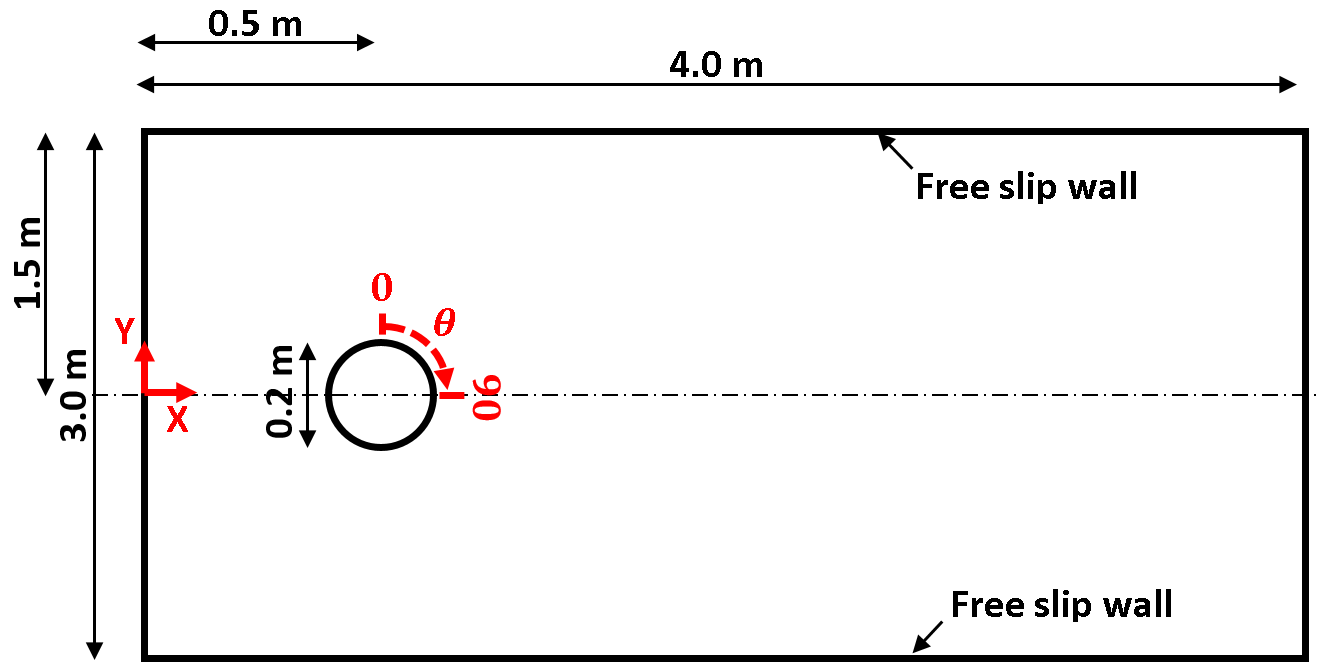
\includegraphics[width=12.00cm]{Chapter_4/figure/flow_over_cylinder/flow_over_cylinder.png}
    \caption{Physical domain with dimensions for flow over cylinder.}
    \label{fig:C4_cylinderPhysicalDomain}
\end{figure}
%
The boundary conditions are defined as the flow velocity at the inlet (left boundary) and the outflow (zero gradient) boundary condition at the outlet (right boundary). The top and bottom boundaries are modeled as free slip walls. The pressure boundary conditions are defined as zero gradient on inlet, top, and bottom wall and zero dirichlet boundary condition at the outlet. The surface of the cylinder is modeled by the virtual boundary method. The cylinder is located at $(0.5, 1.5)$ and has the radius of $0.1 m$. Its surface is represented by using 50 Lagrangian nodes. The $\alpha$ and $\beta$ values for this analysis are selected as $-10^4$ and $-50$, respectively. These constants are problem dependent and are selected in such a way that the required velocity conditions are satisfied at the Lagrangian points. To ensure the stability of the numerical method, the CFL number is kept under one for all following analysis. This is done by selecting an appropriate time step for the chosen mesh size using Equation \eqref{eq:C4_CFLnumber}.
%
\begin{equation}\label{eq:C4_CFLnumber}
	\frac{u \Delta t}{\Delta x} + \frac{v \Delta t}{\Delta y} \leq 1.0
\end{equation}
%
The mesh convergence for this problem for a Reynolds number of 100 is shown in Figure \ref{fig:C4_meshConvergenceForCylidnerRE100GE}.
%
\begin{figure}[H]
    \centering
    \subfigure[U-velocity on y = 1.5]
    {
    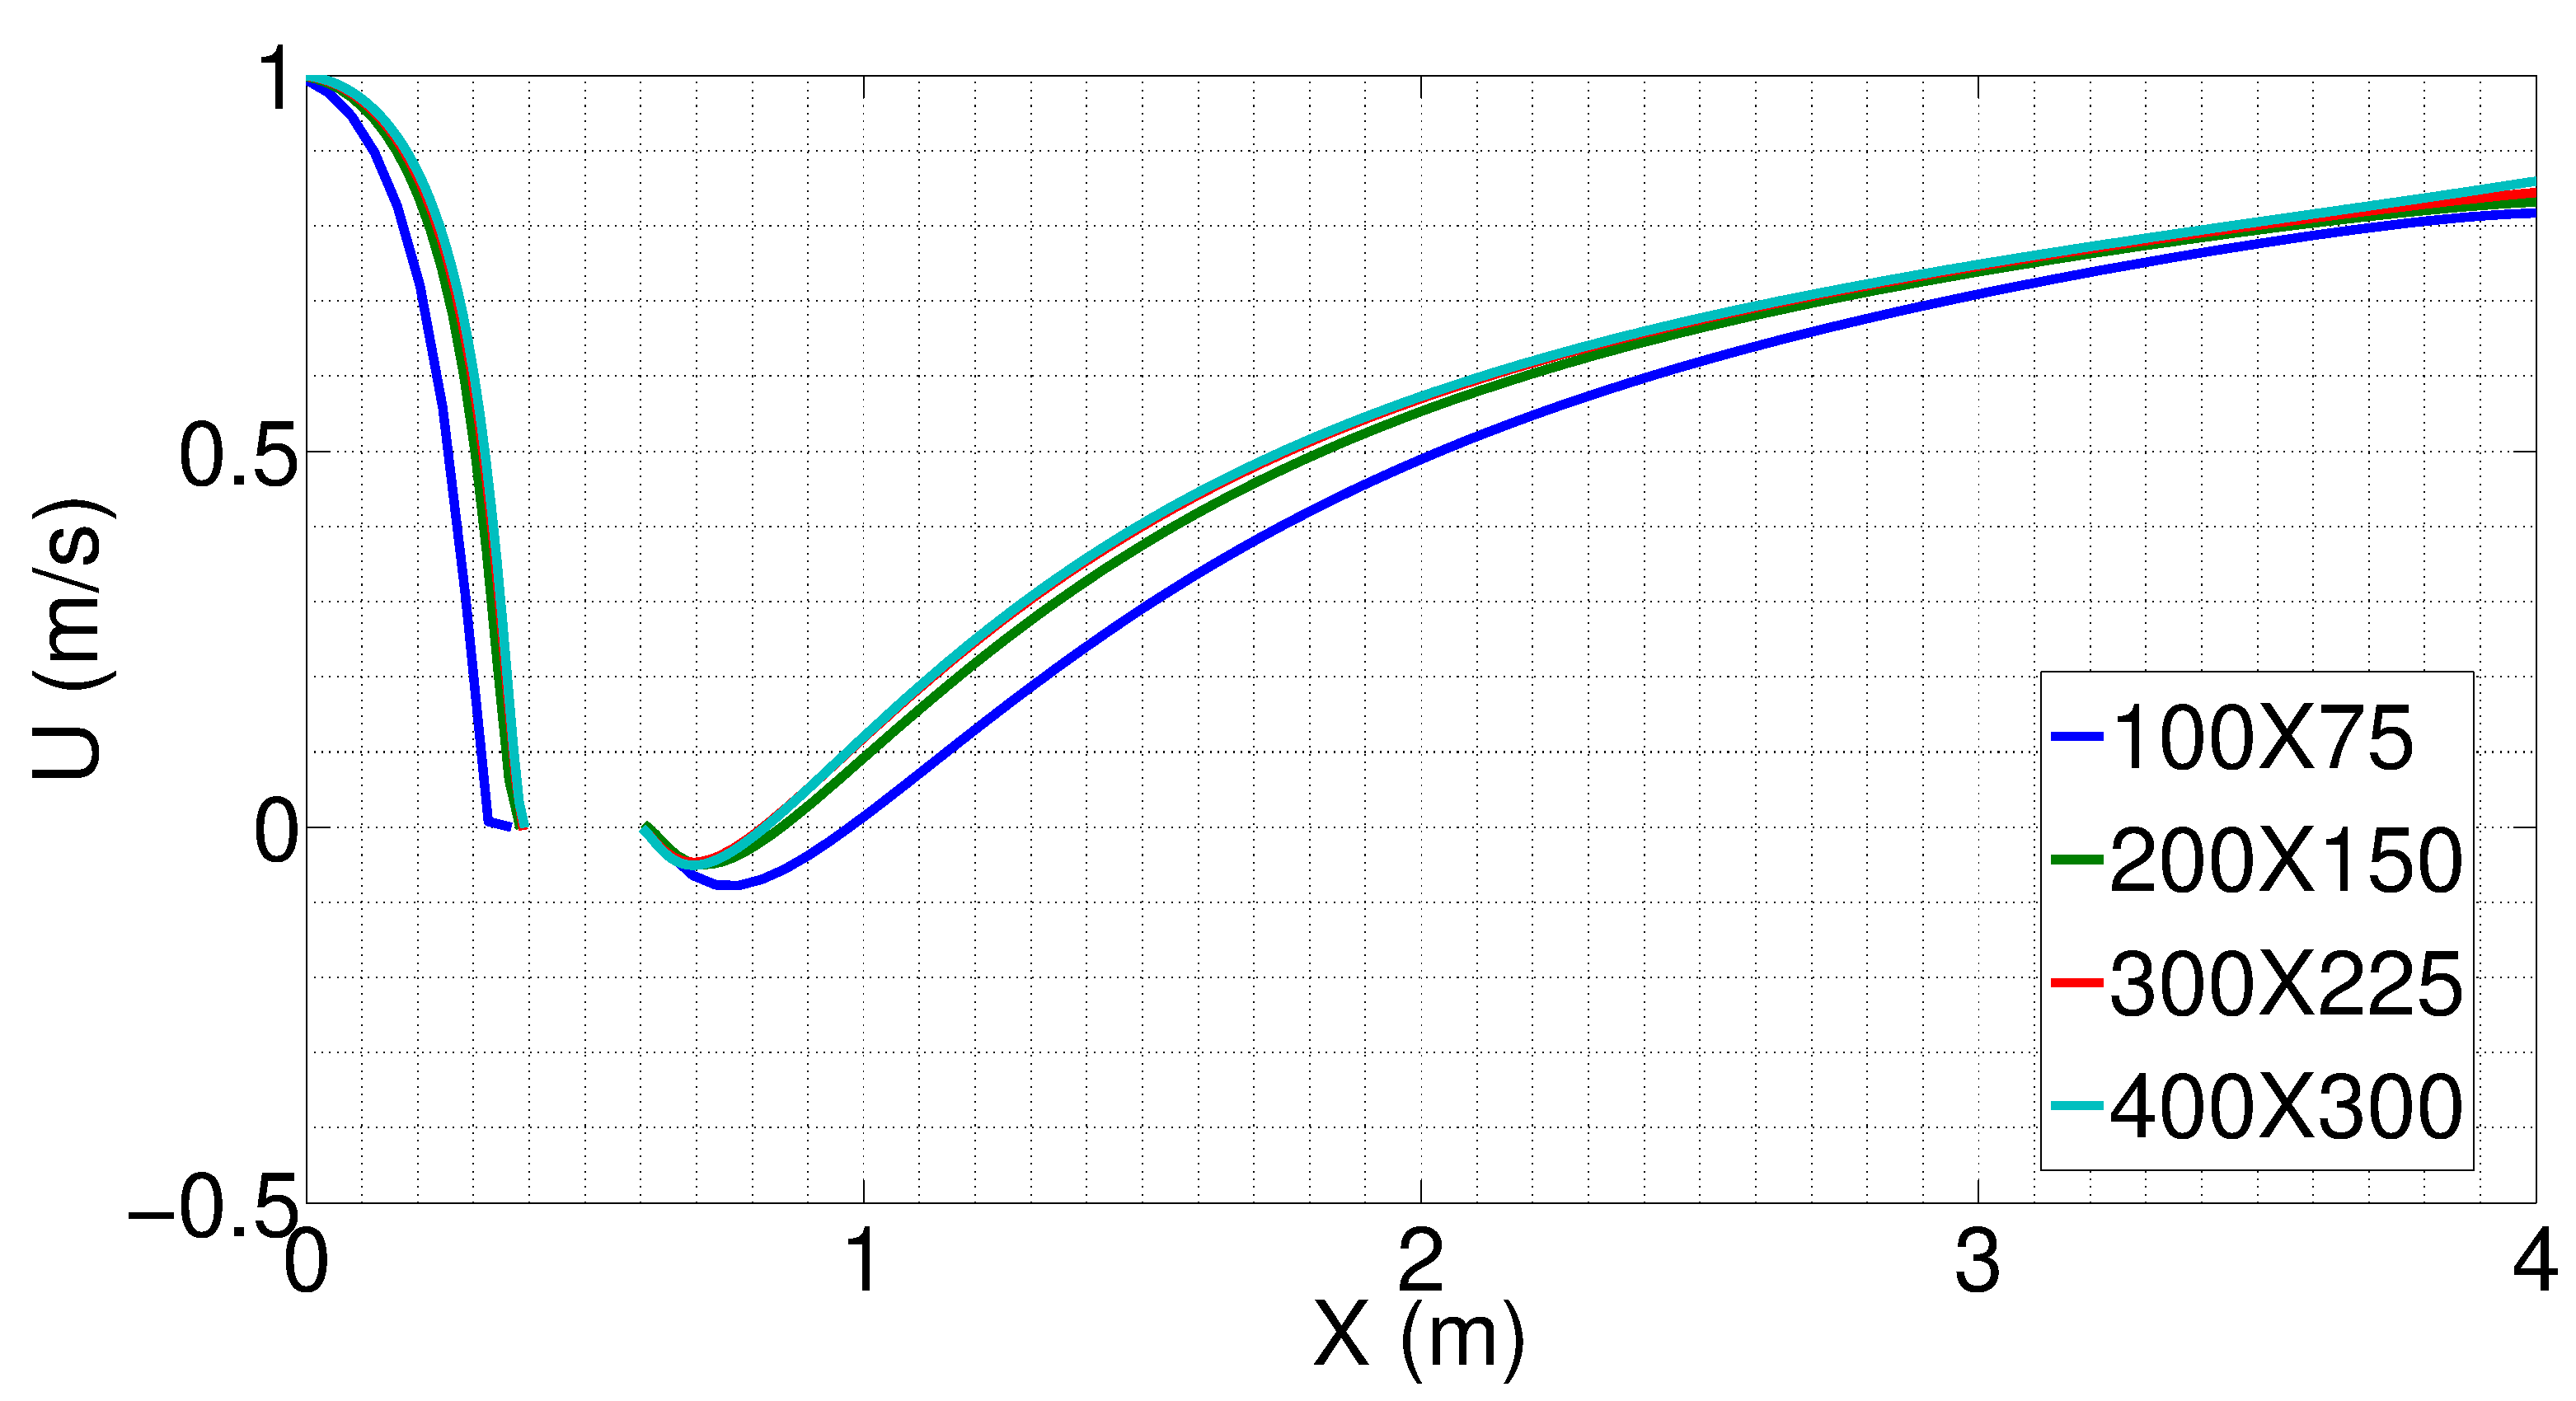
\includegraphics[width=6.5cm]{Chapter_4/figure/flow_over_cylinder/meshConvergence_RE100_U.eps}
    }
    \quad
    \subfigure[V-velocity on x = 2.0]
    {
    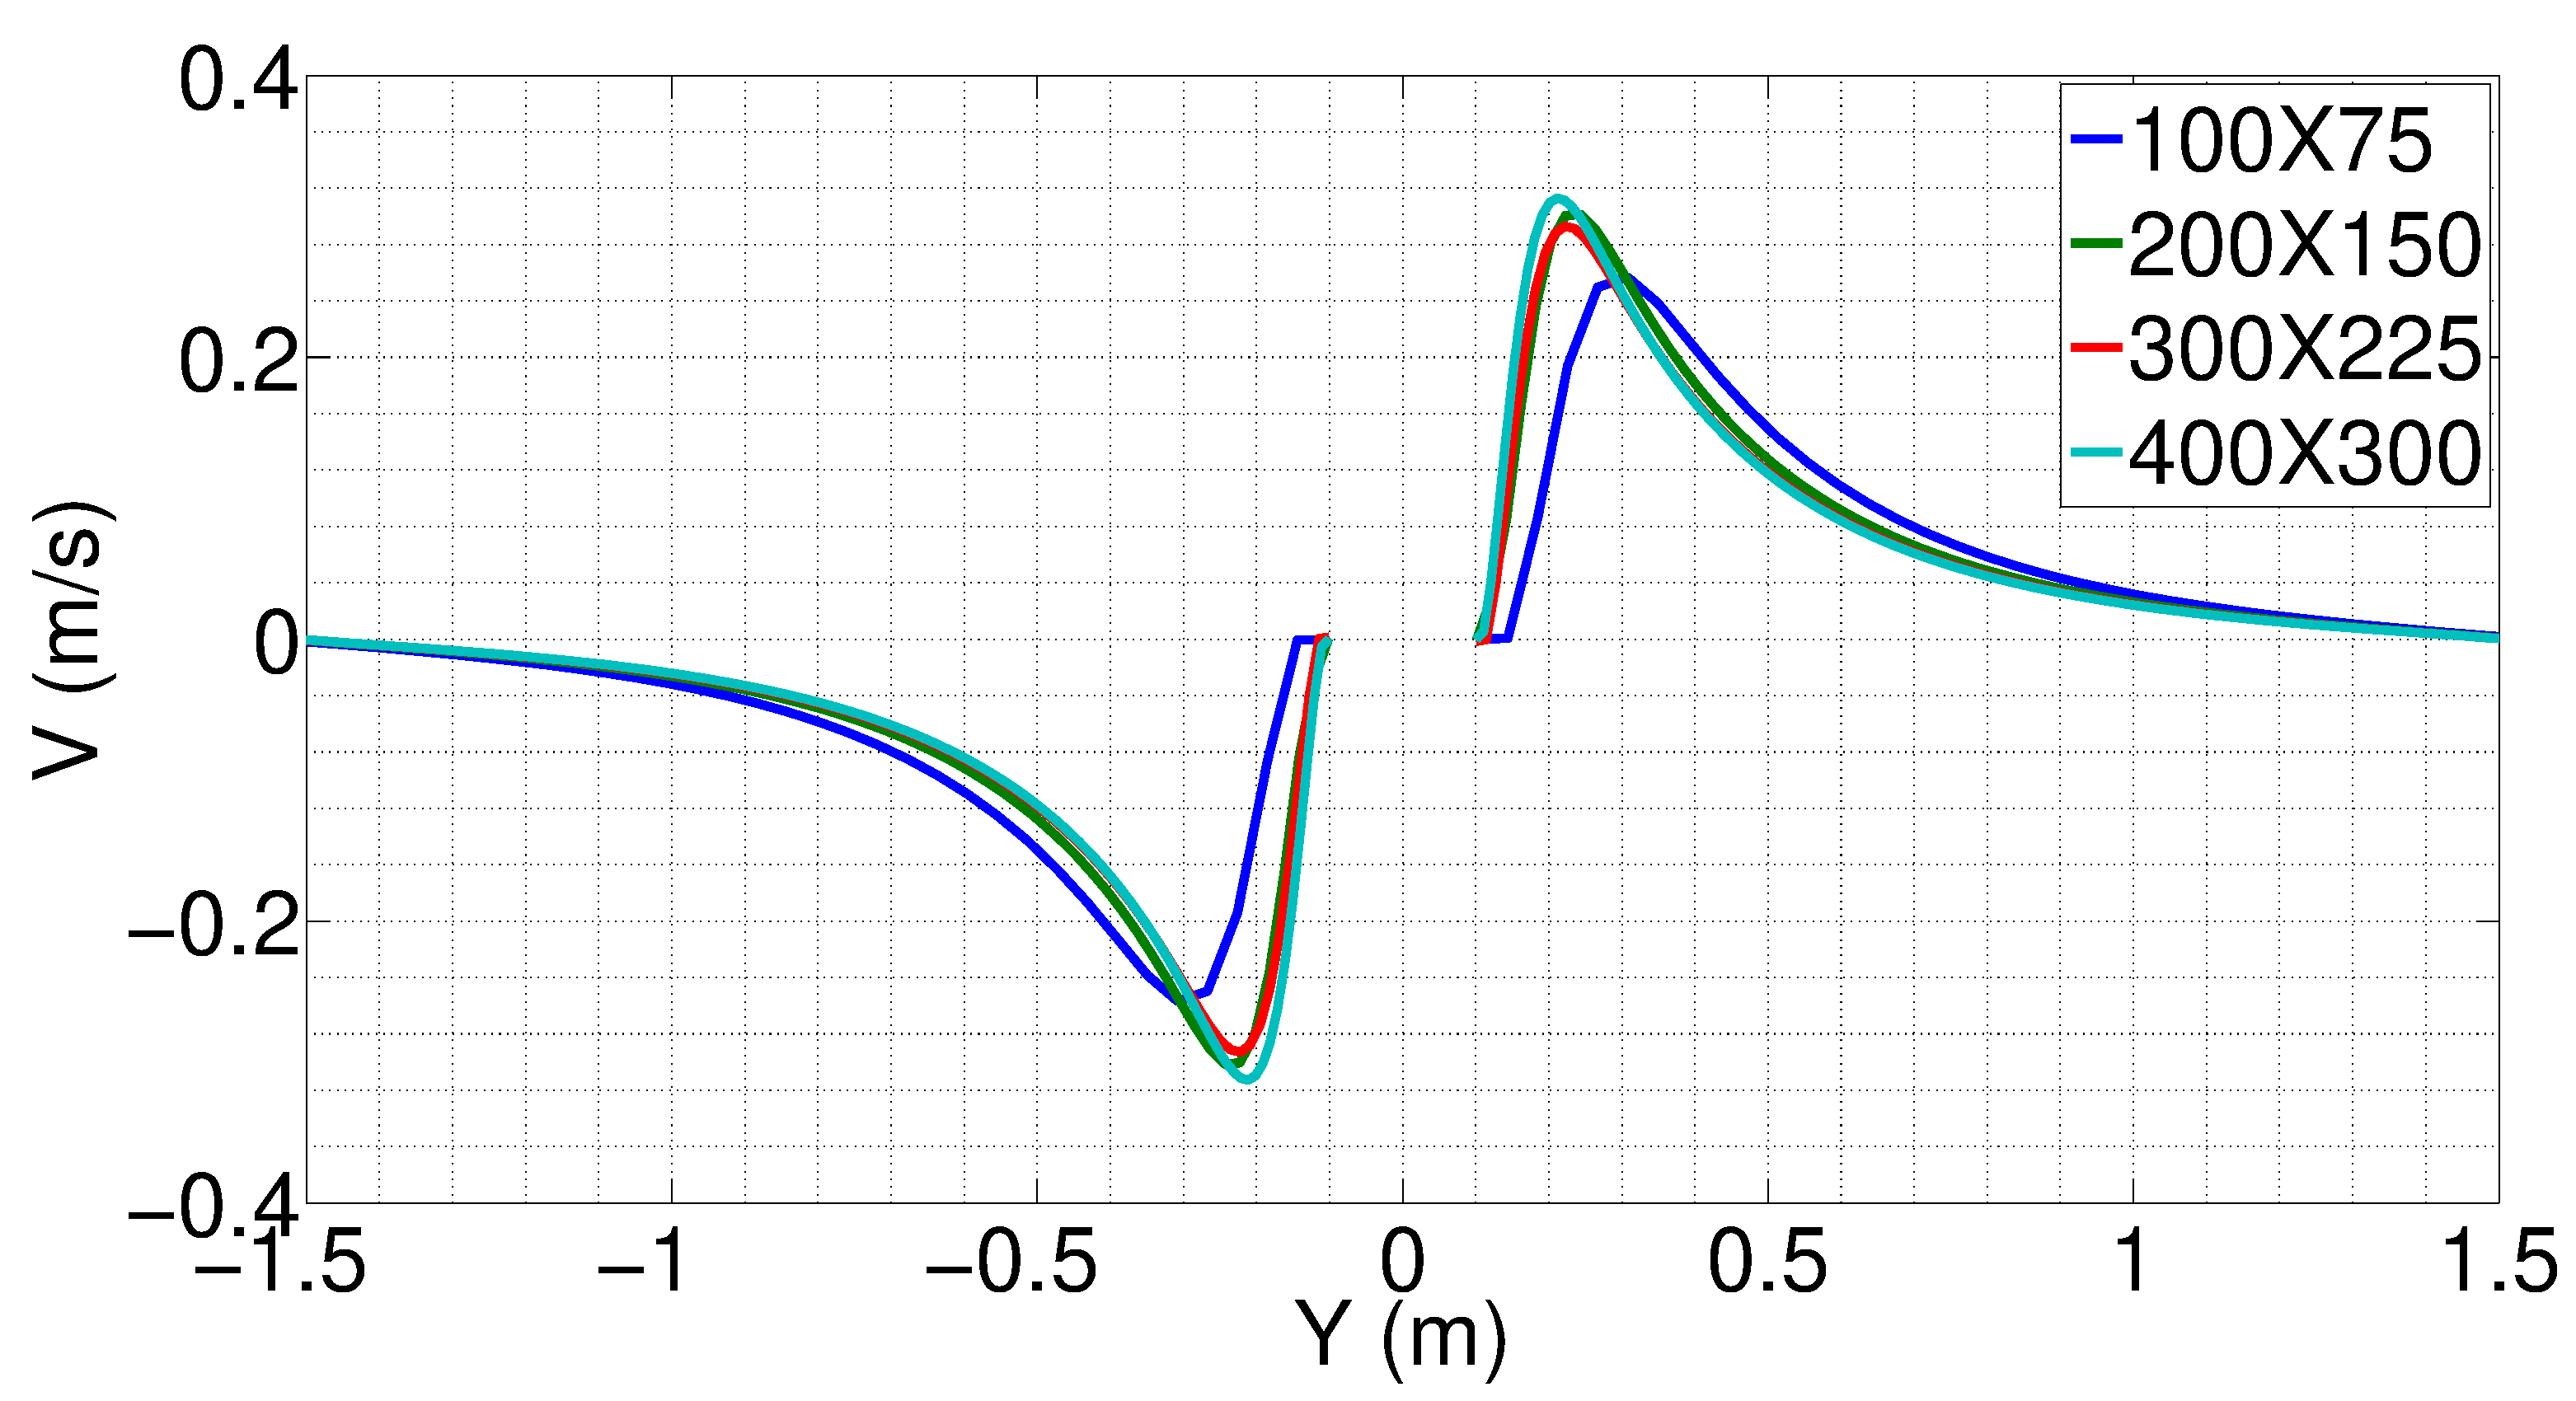
\includegraphics[width=6.5cm]{Chapter_4/figure/flow_over_cylinder/meshConvergence_RE100_V.eps}
    }
    \\
    \subfigure[Pressure on x = 2.0]
    {
    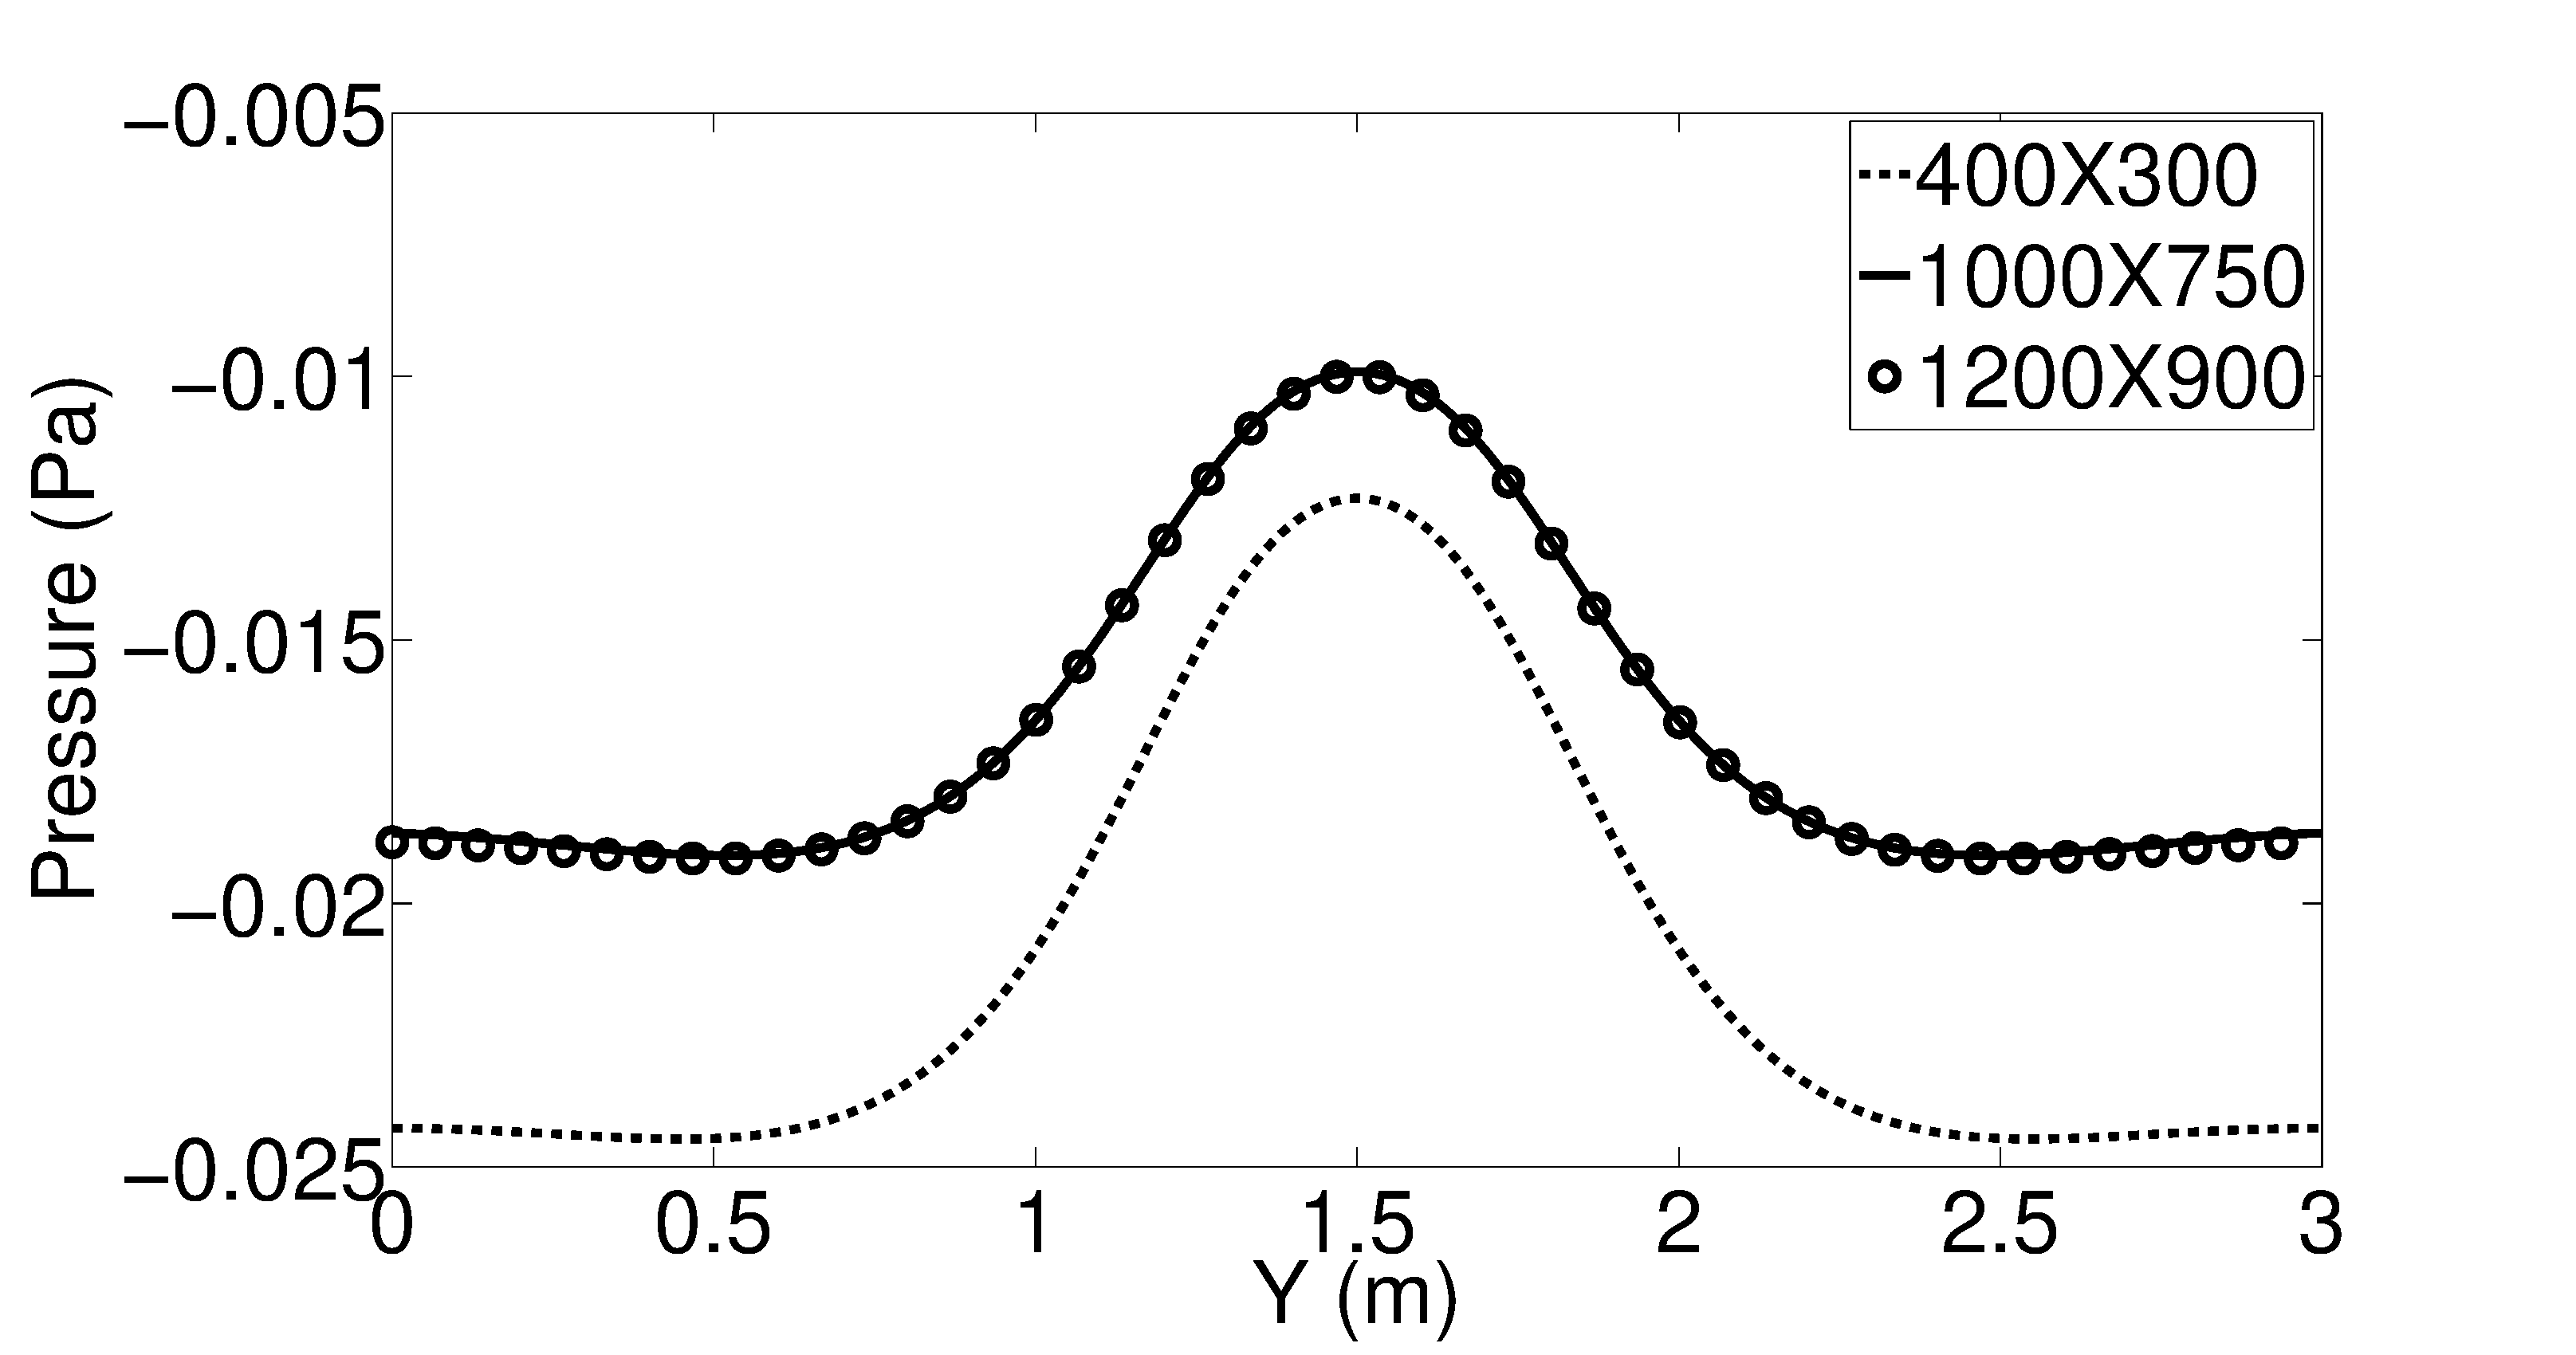
\includegraphics[width=6.5cm]{Chapter_4/figure/flow_over_cylinder/meshConvergence_RE100_P1.eps}
    }
    \subfigure[Pressure on y = 1.5]
    {
    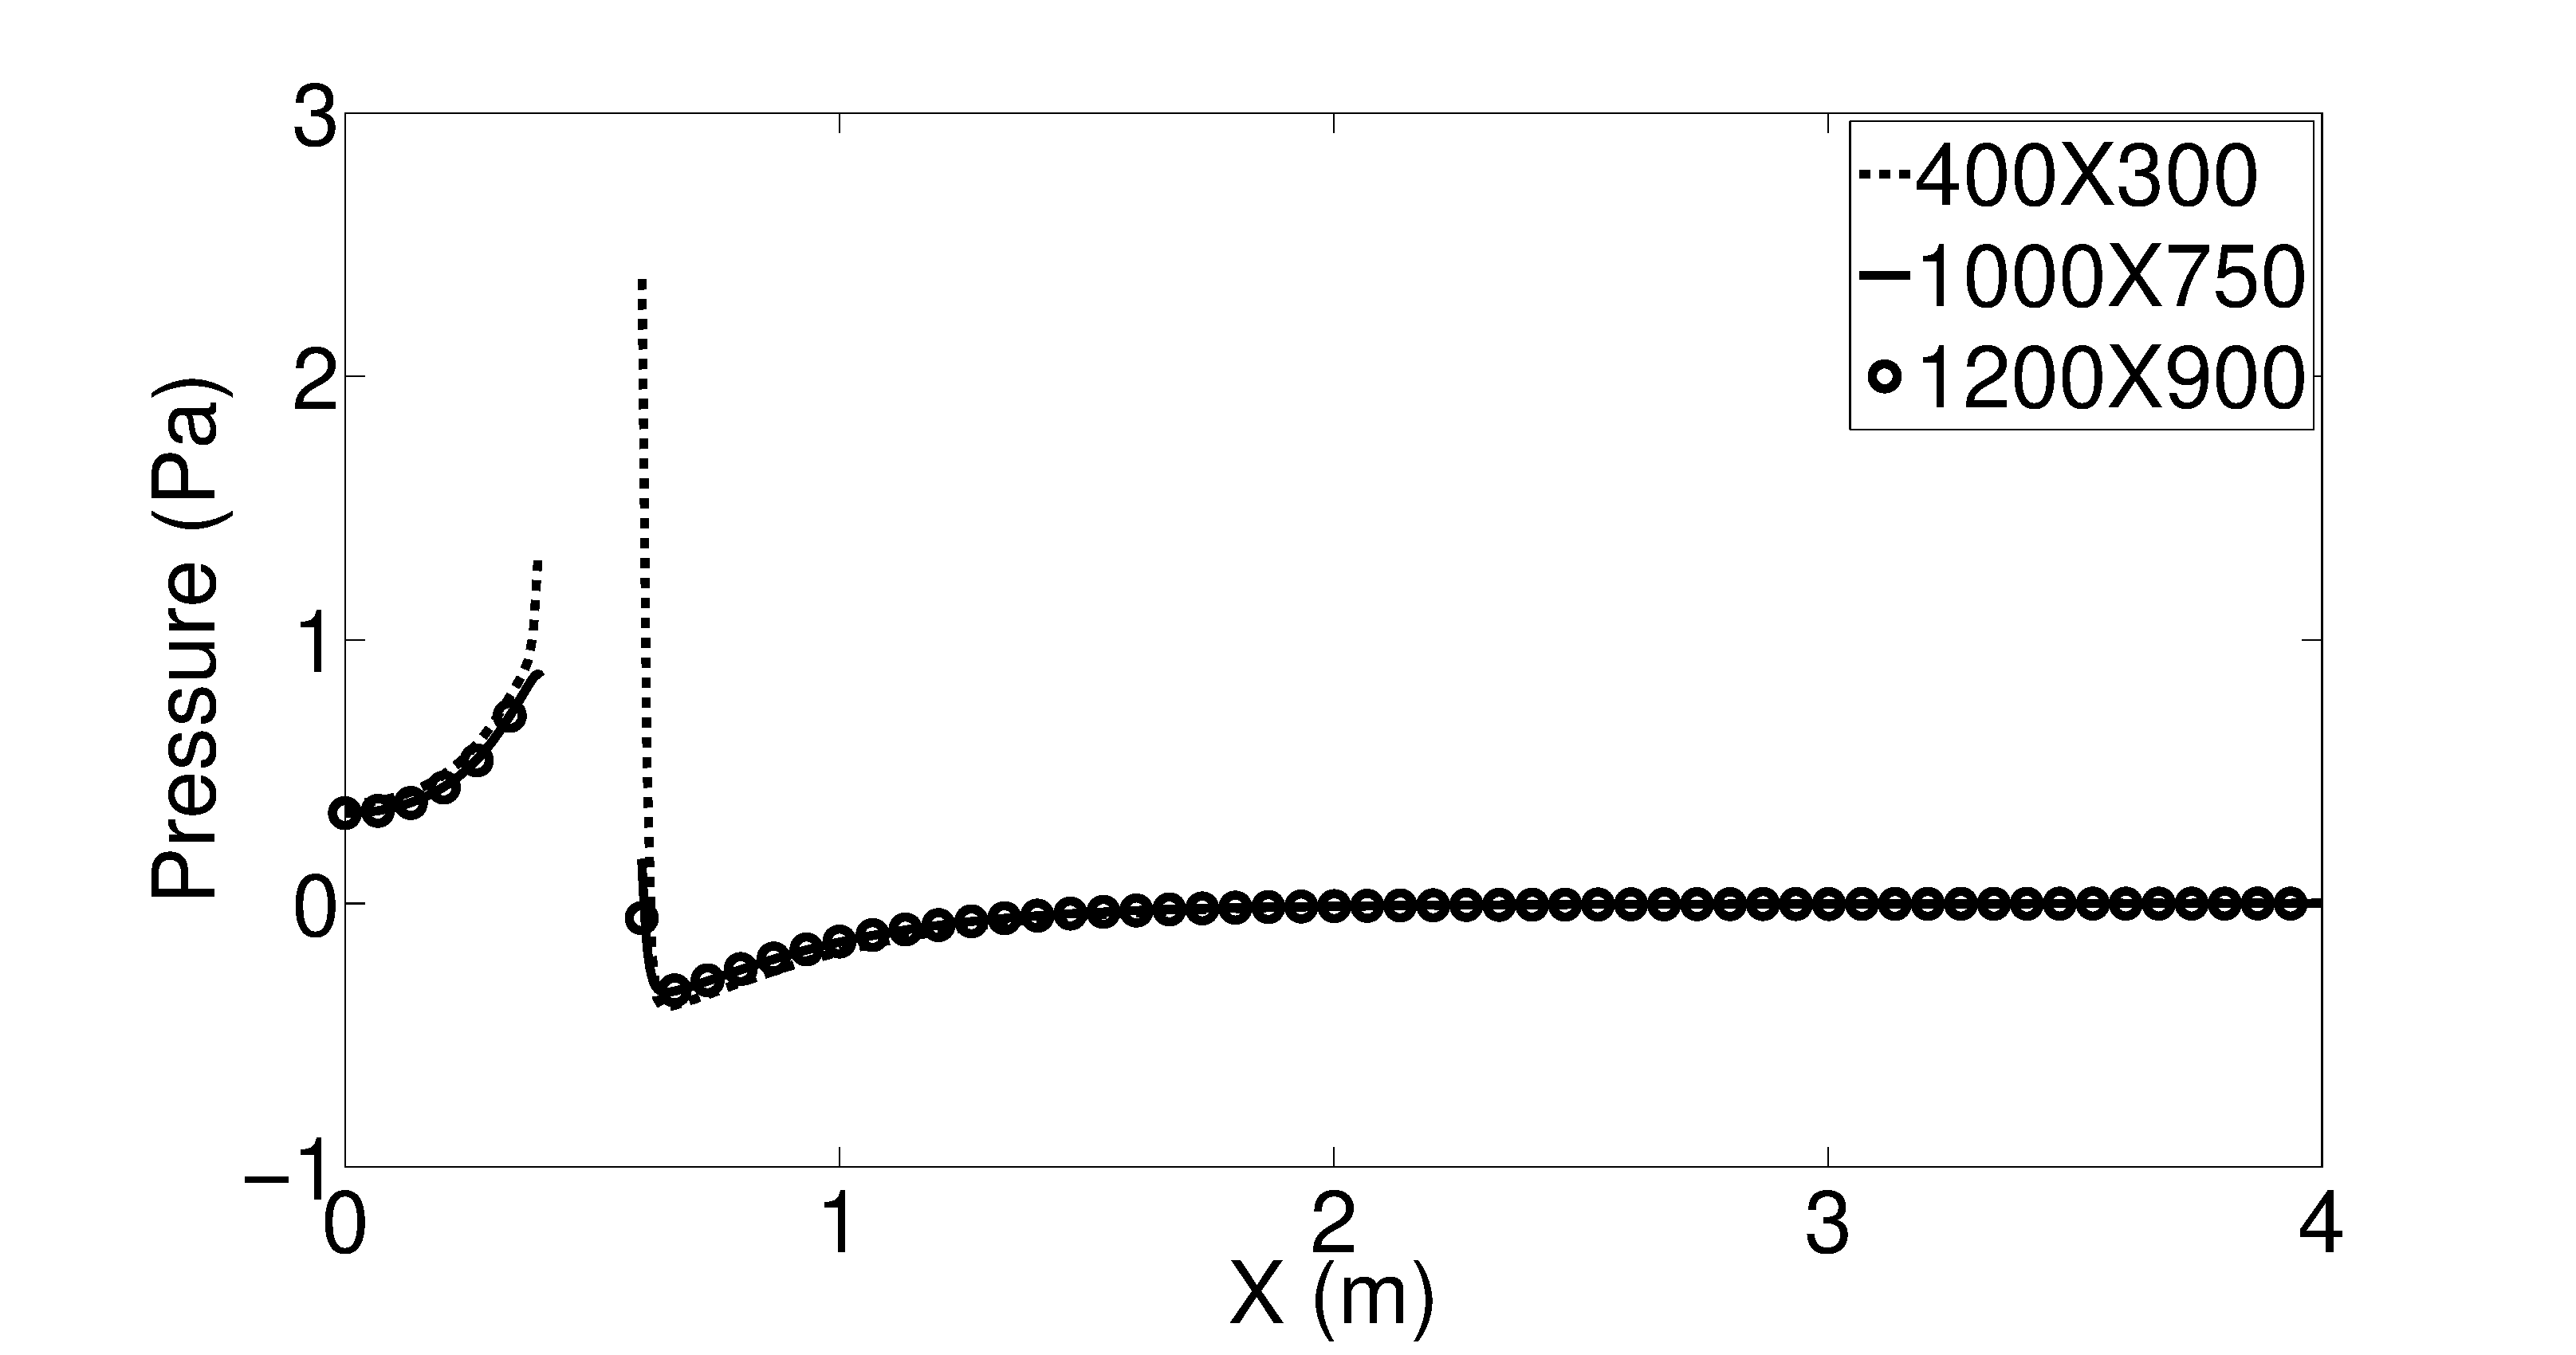
\includegraphics[width=6.5cm]{Chapter_4/figure/flow_over_cylinder/meshConvergence_RE100_P2.eps}
    }
    \caption{Convergence results for Re = 100.}
    \label{fig:C4_meshConvergenceForCylidnerRE100GE}
\end{figure}
%
The convergence study of the mesh refinement is also conducted for a node on the downwash of the cylinder at $(2, 0)$ as shown in Figure \ref{fig:C4_meshRefinementForCylinderRE100GE}. The slopes of the fitted curves to the u-velocity, v-velocity, and pressure error estimates are calculated as $-2.34$, $-1.96$, and $-2.72$, respectfully. This means that the method is second-order accurate in space and time.
%
\begin{figure}[H]
    \centering
    \subfigure[U-velocity convergence on $(2.0, 0)$.]
    {
    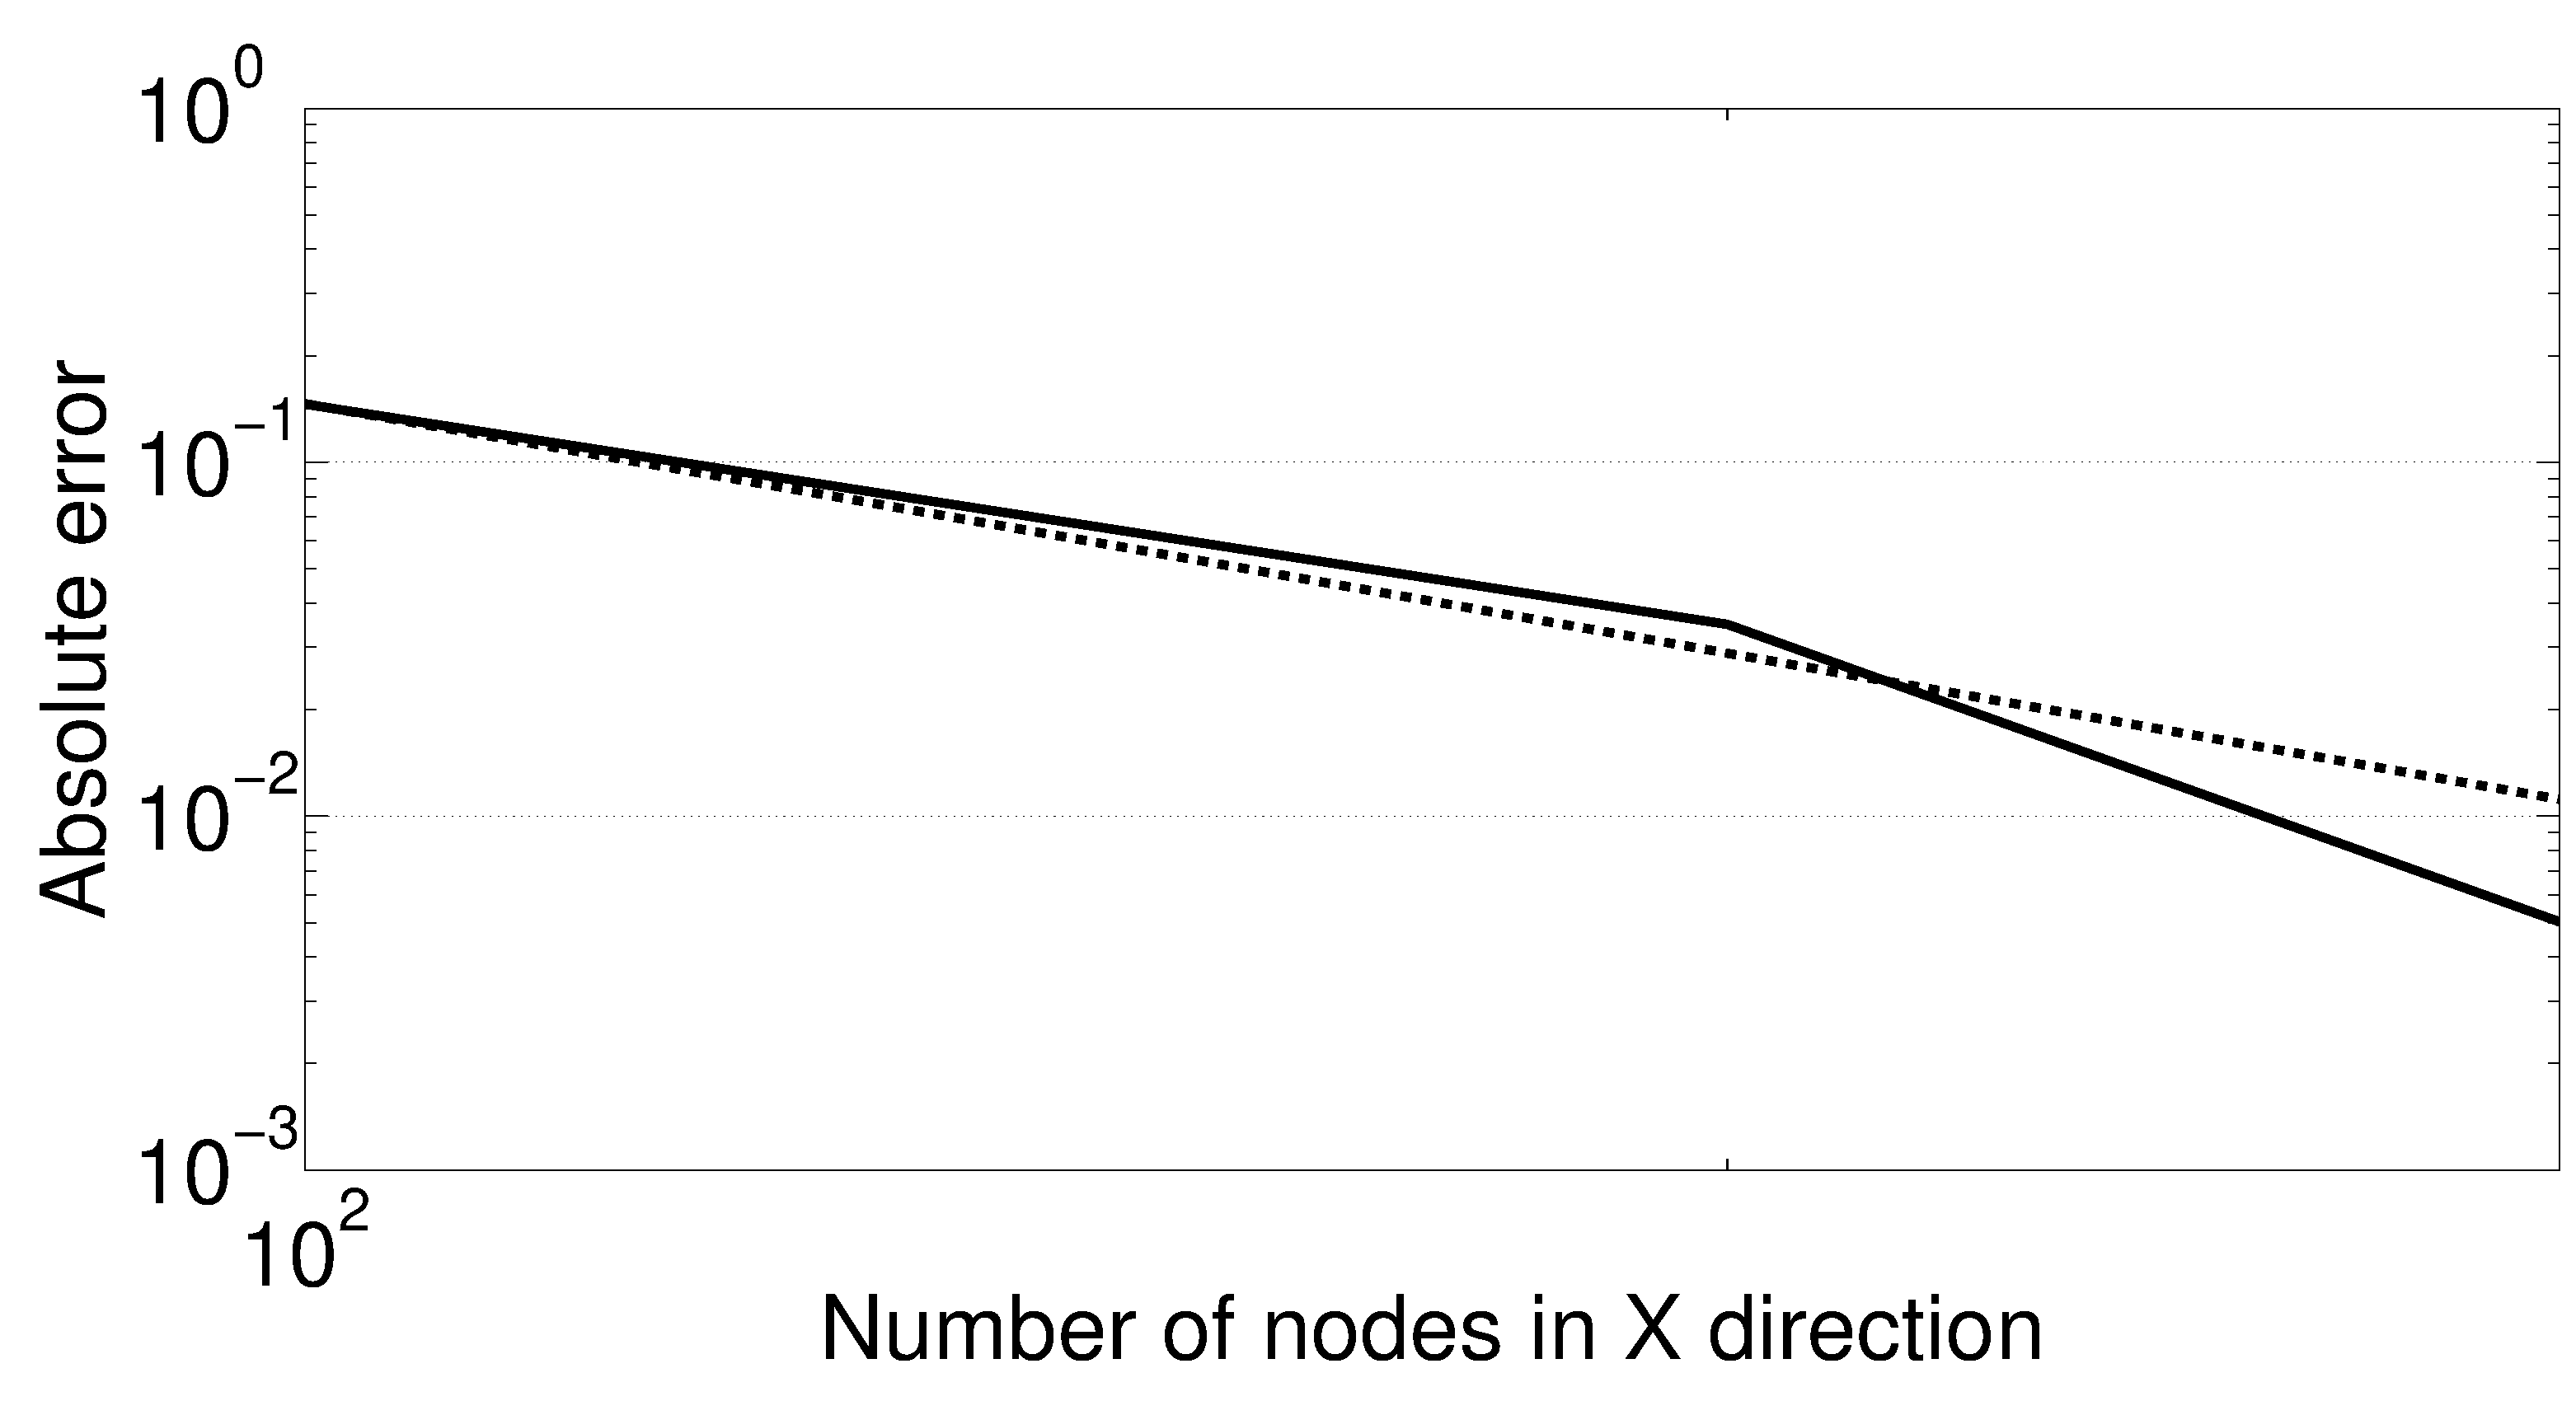
\includegraphics[width=6.5cm]{Chapter_4/figure/flow_over_cylinder/u_convergence_RE100.eps}
    }
    \quad
    \subfigure[V-velocity convergence on $(0.5, 0.75)$.]
    {
    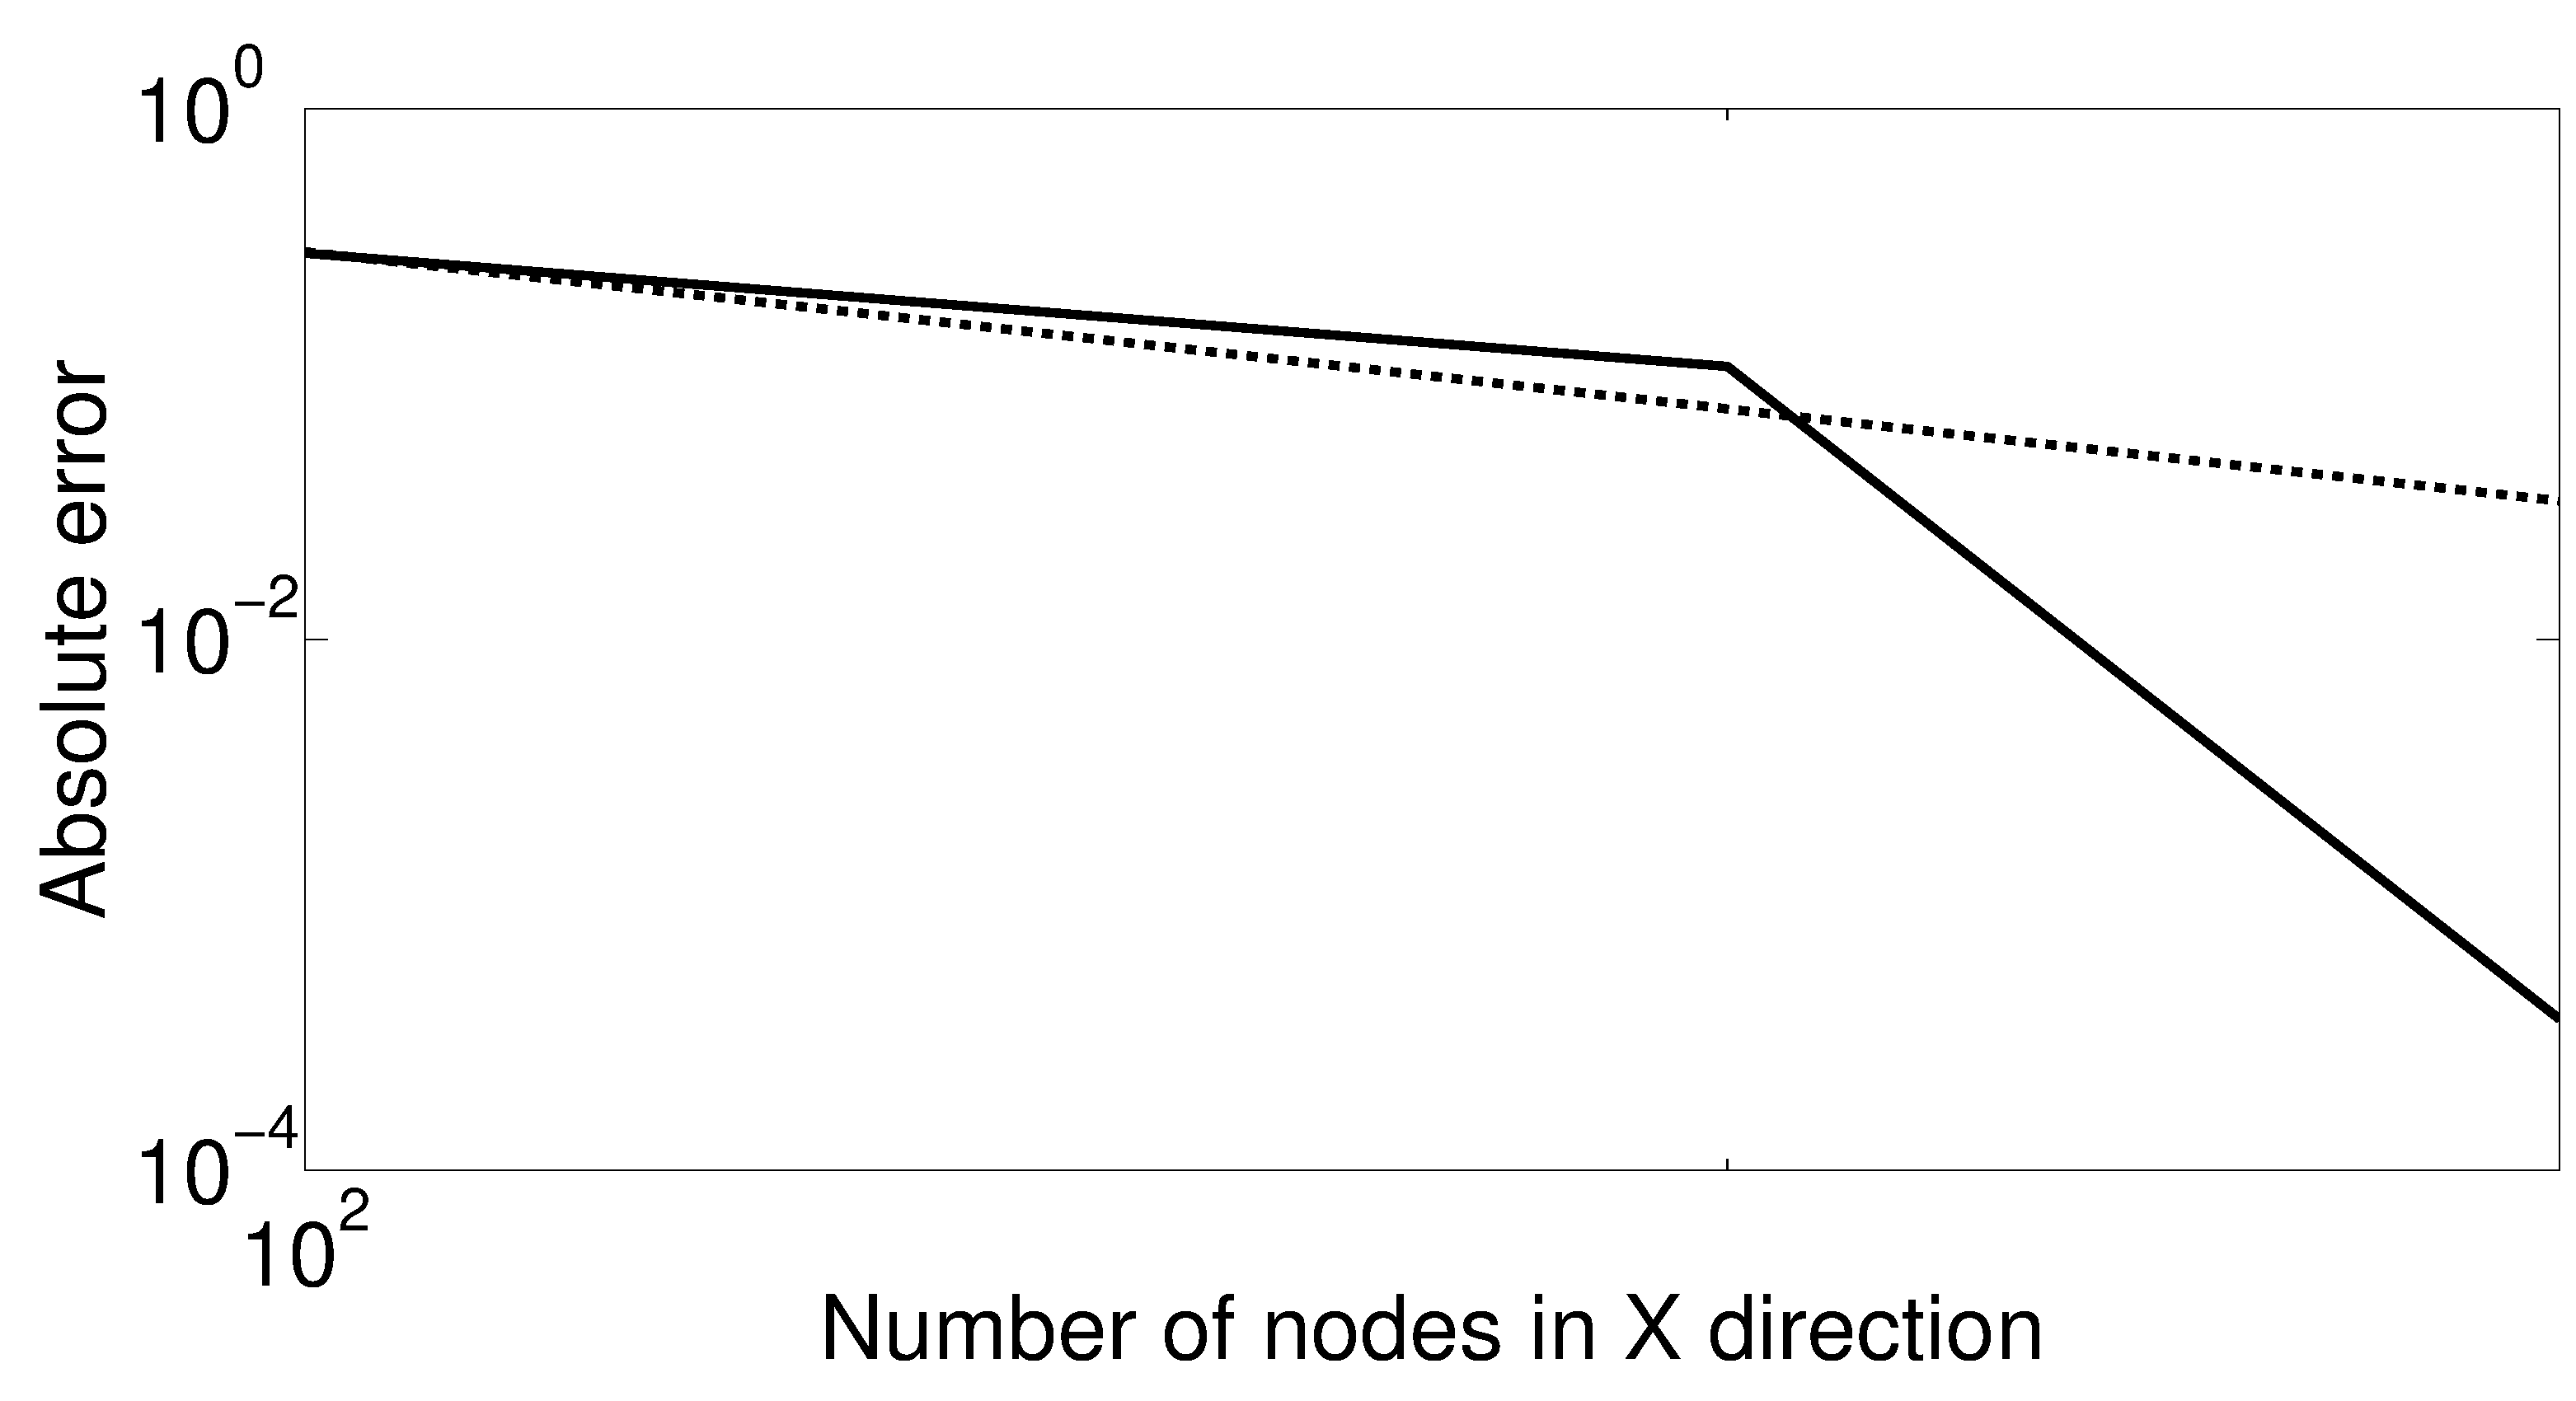
\includegraphics[width=6.5cm]{Chapter_4/figure/flow_over_cylinder/v_convergence_RE100.eps}
    }
    \\
    \subfigure[Pressure convergence on $(2.0, 0)$.]
    {
    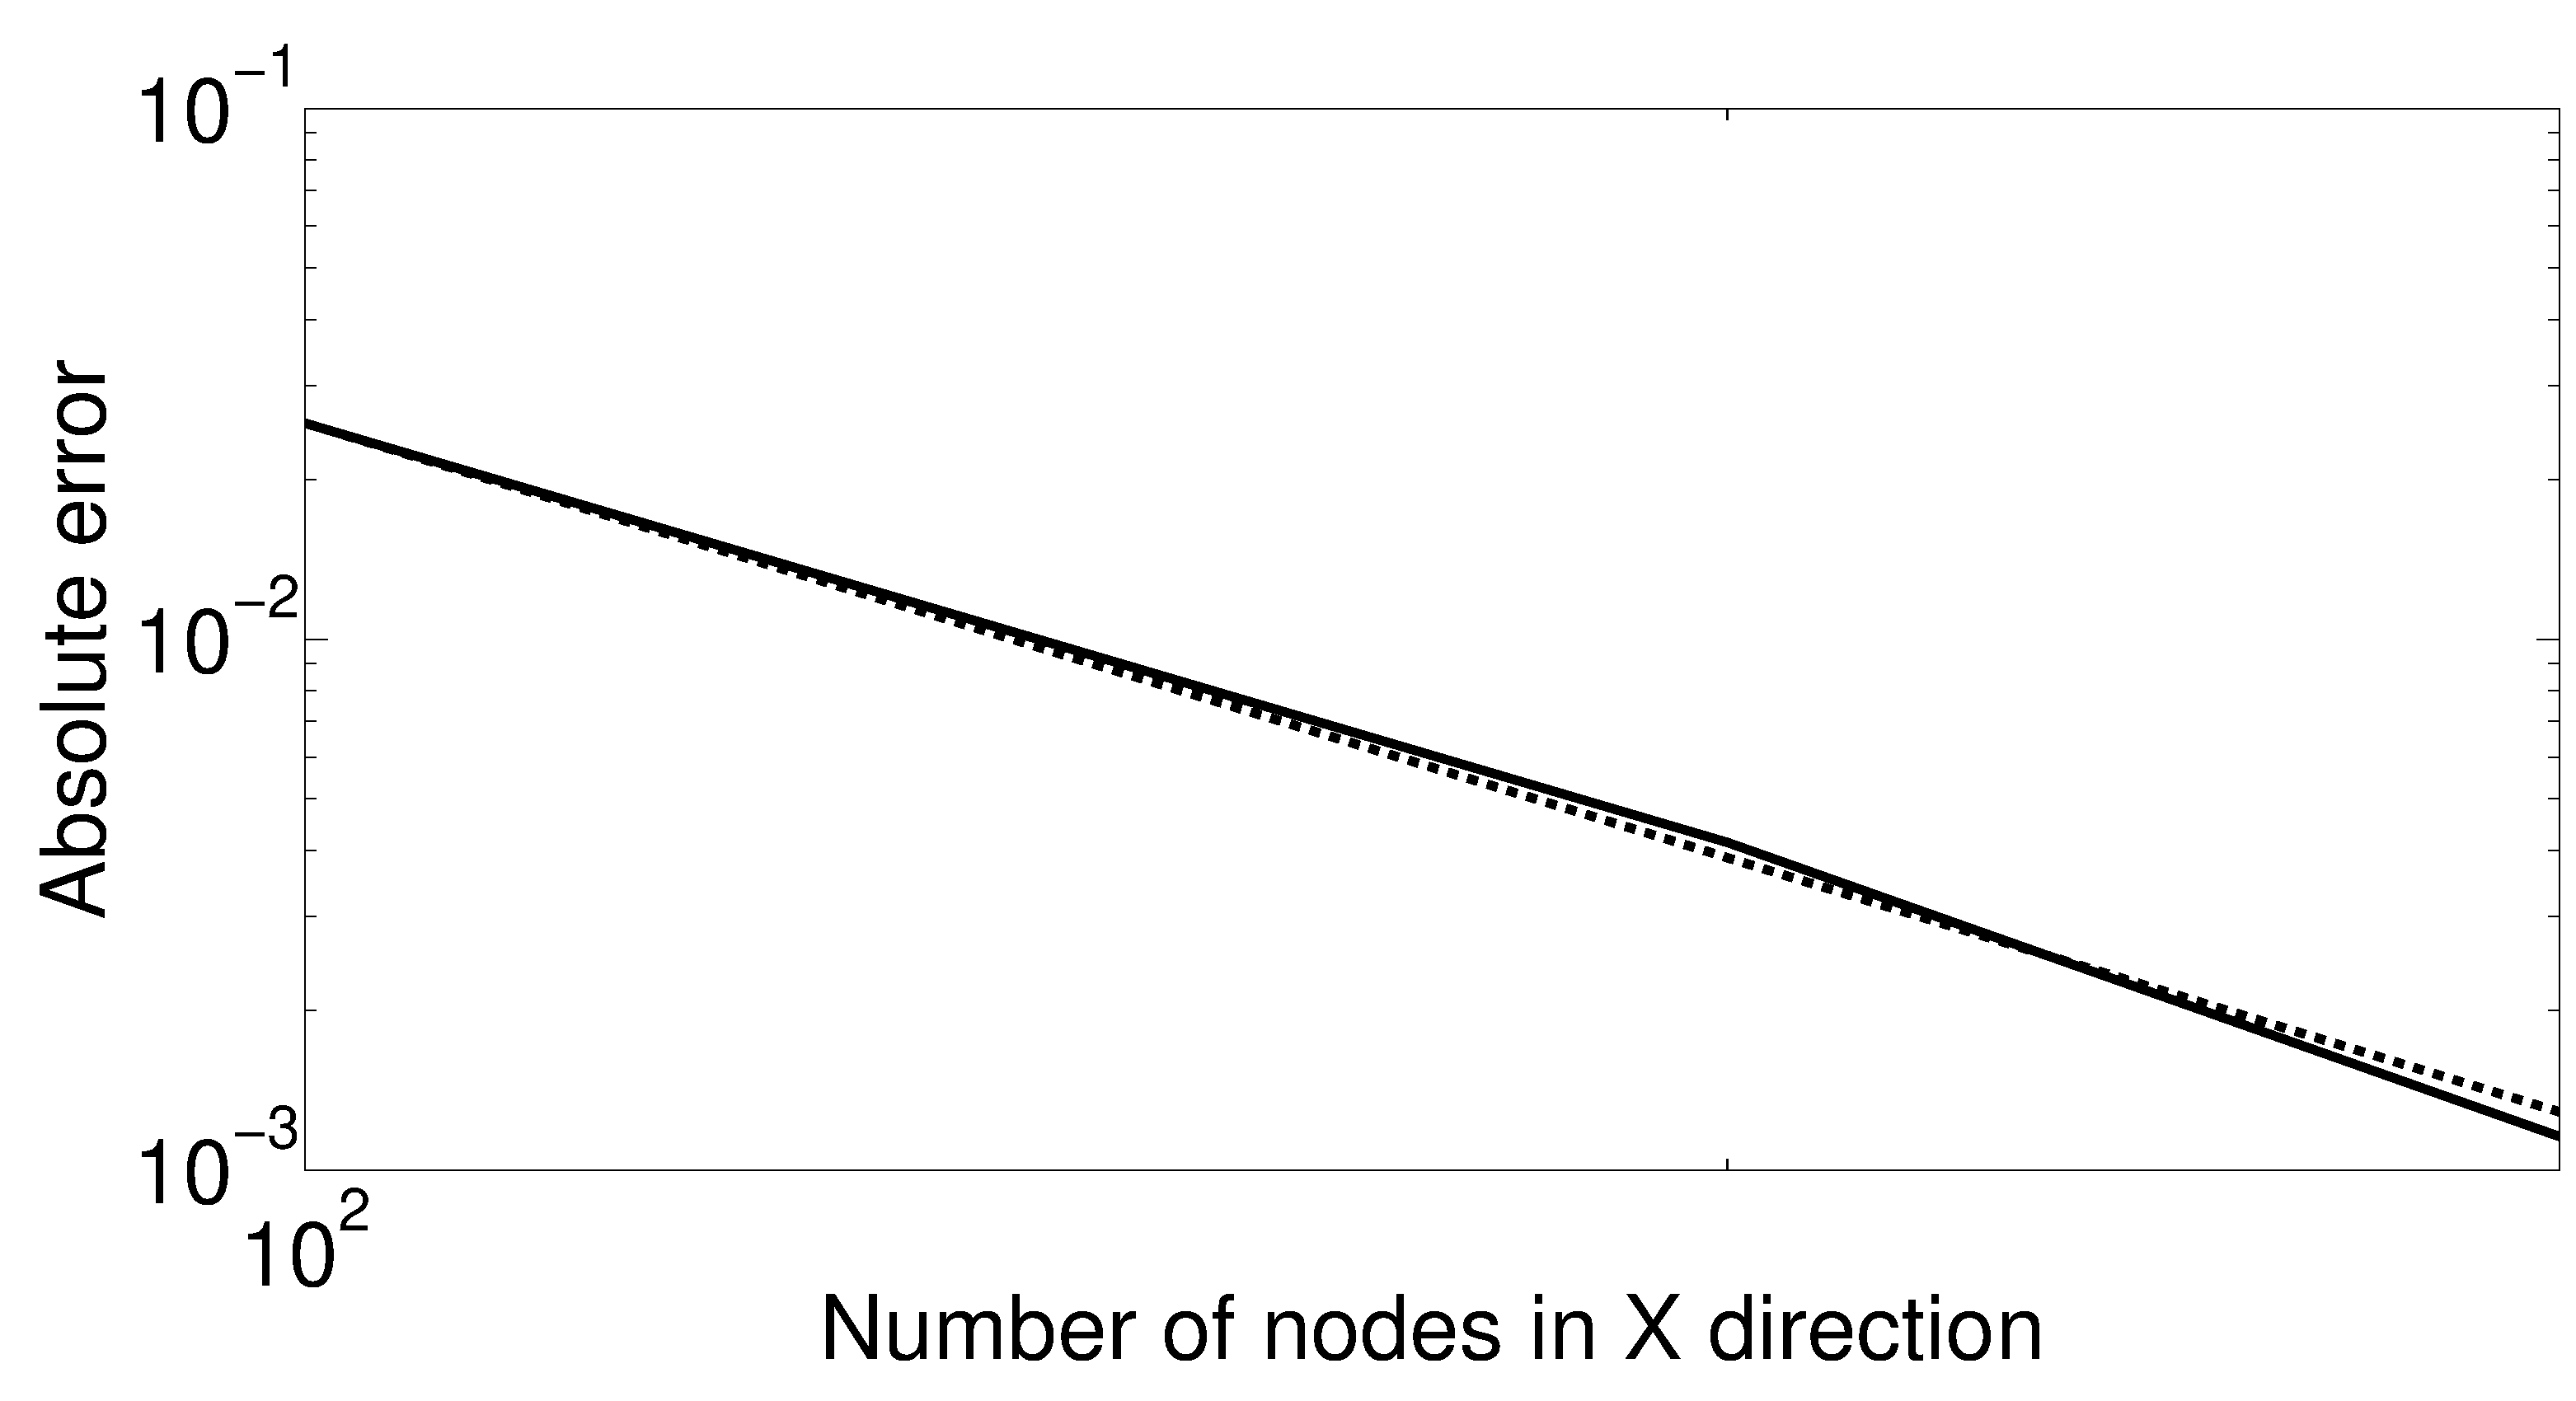
\includegraphics[width=6.5cm]{Chapter_4/figure/flow_over_cylinder/pressure_convergence_RE100.eps}
    }
    \caption{Convergence plots for Re = 100.}
    \label{fig:C4_meshRefinementForCylinderRE100GE}
\end{figure}
%
The contour plots for the velocity and pressure are shown in Figure \ref{fig:C4_contourPlotsForFlowOverCylidnerGE}.
%
\begin{figure}[H]
    \centering
    \subfigure[U-velocity]
    {
    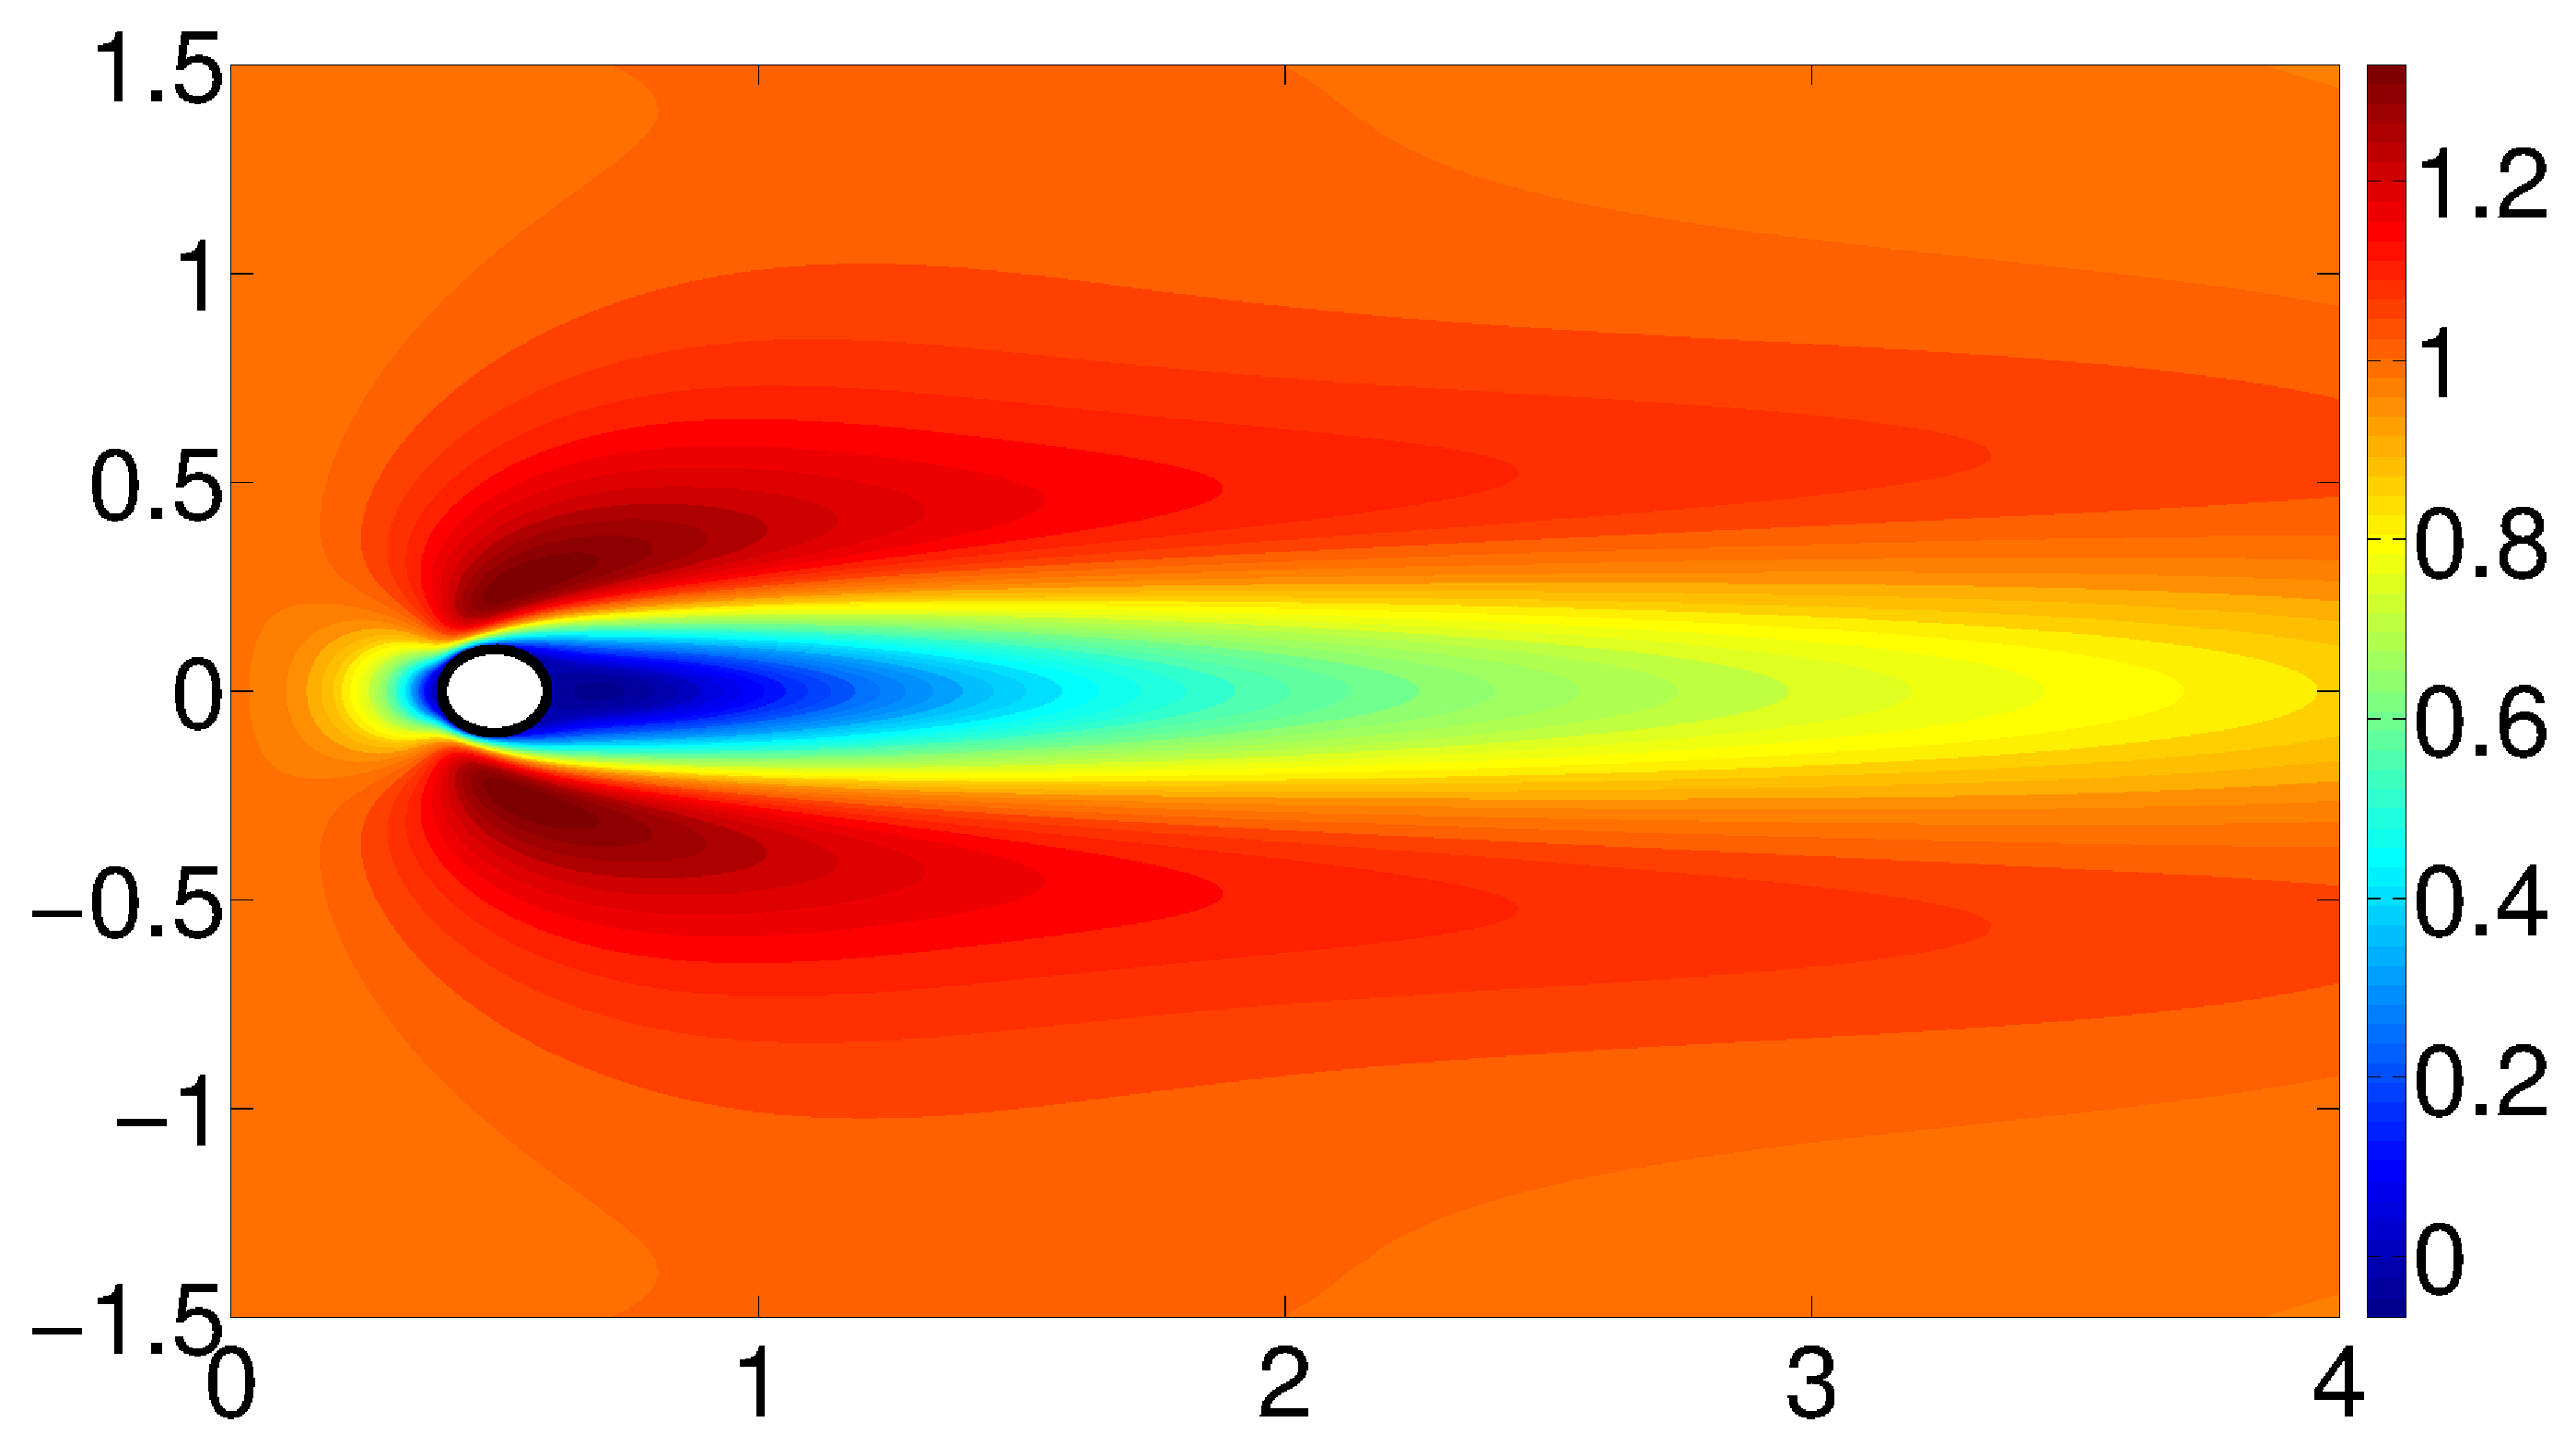
\includegraphics[width=6.5cm]{Chapter_4/figure/flow_over_cylinder/u_velocity_contour_RE100.eps}
    }
    \quad
    \subfigure[V-velocity]
    {
    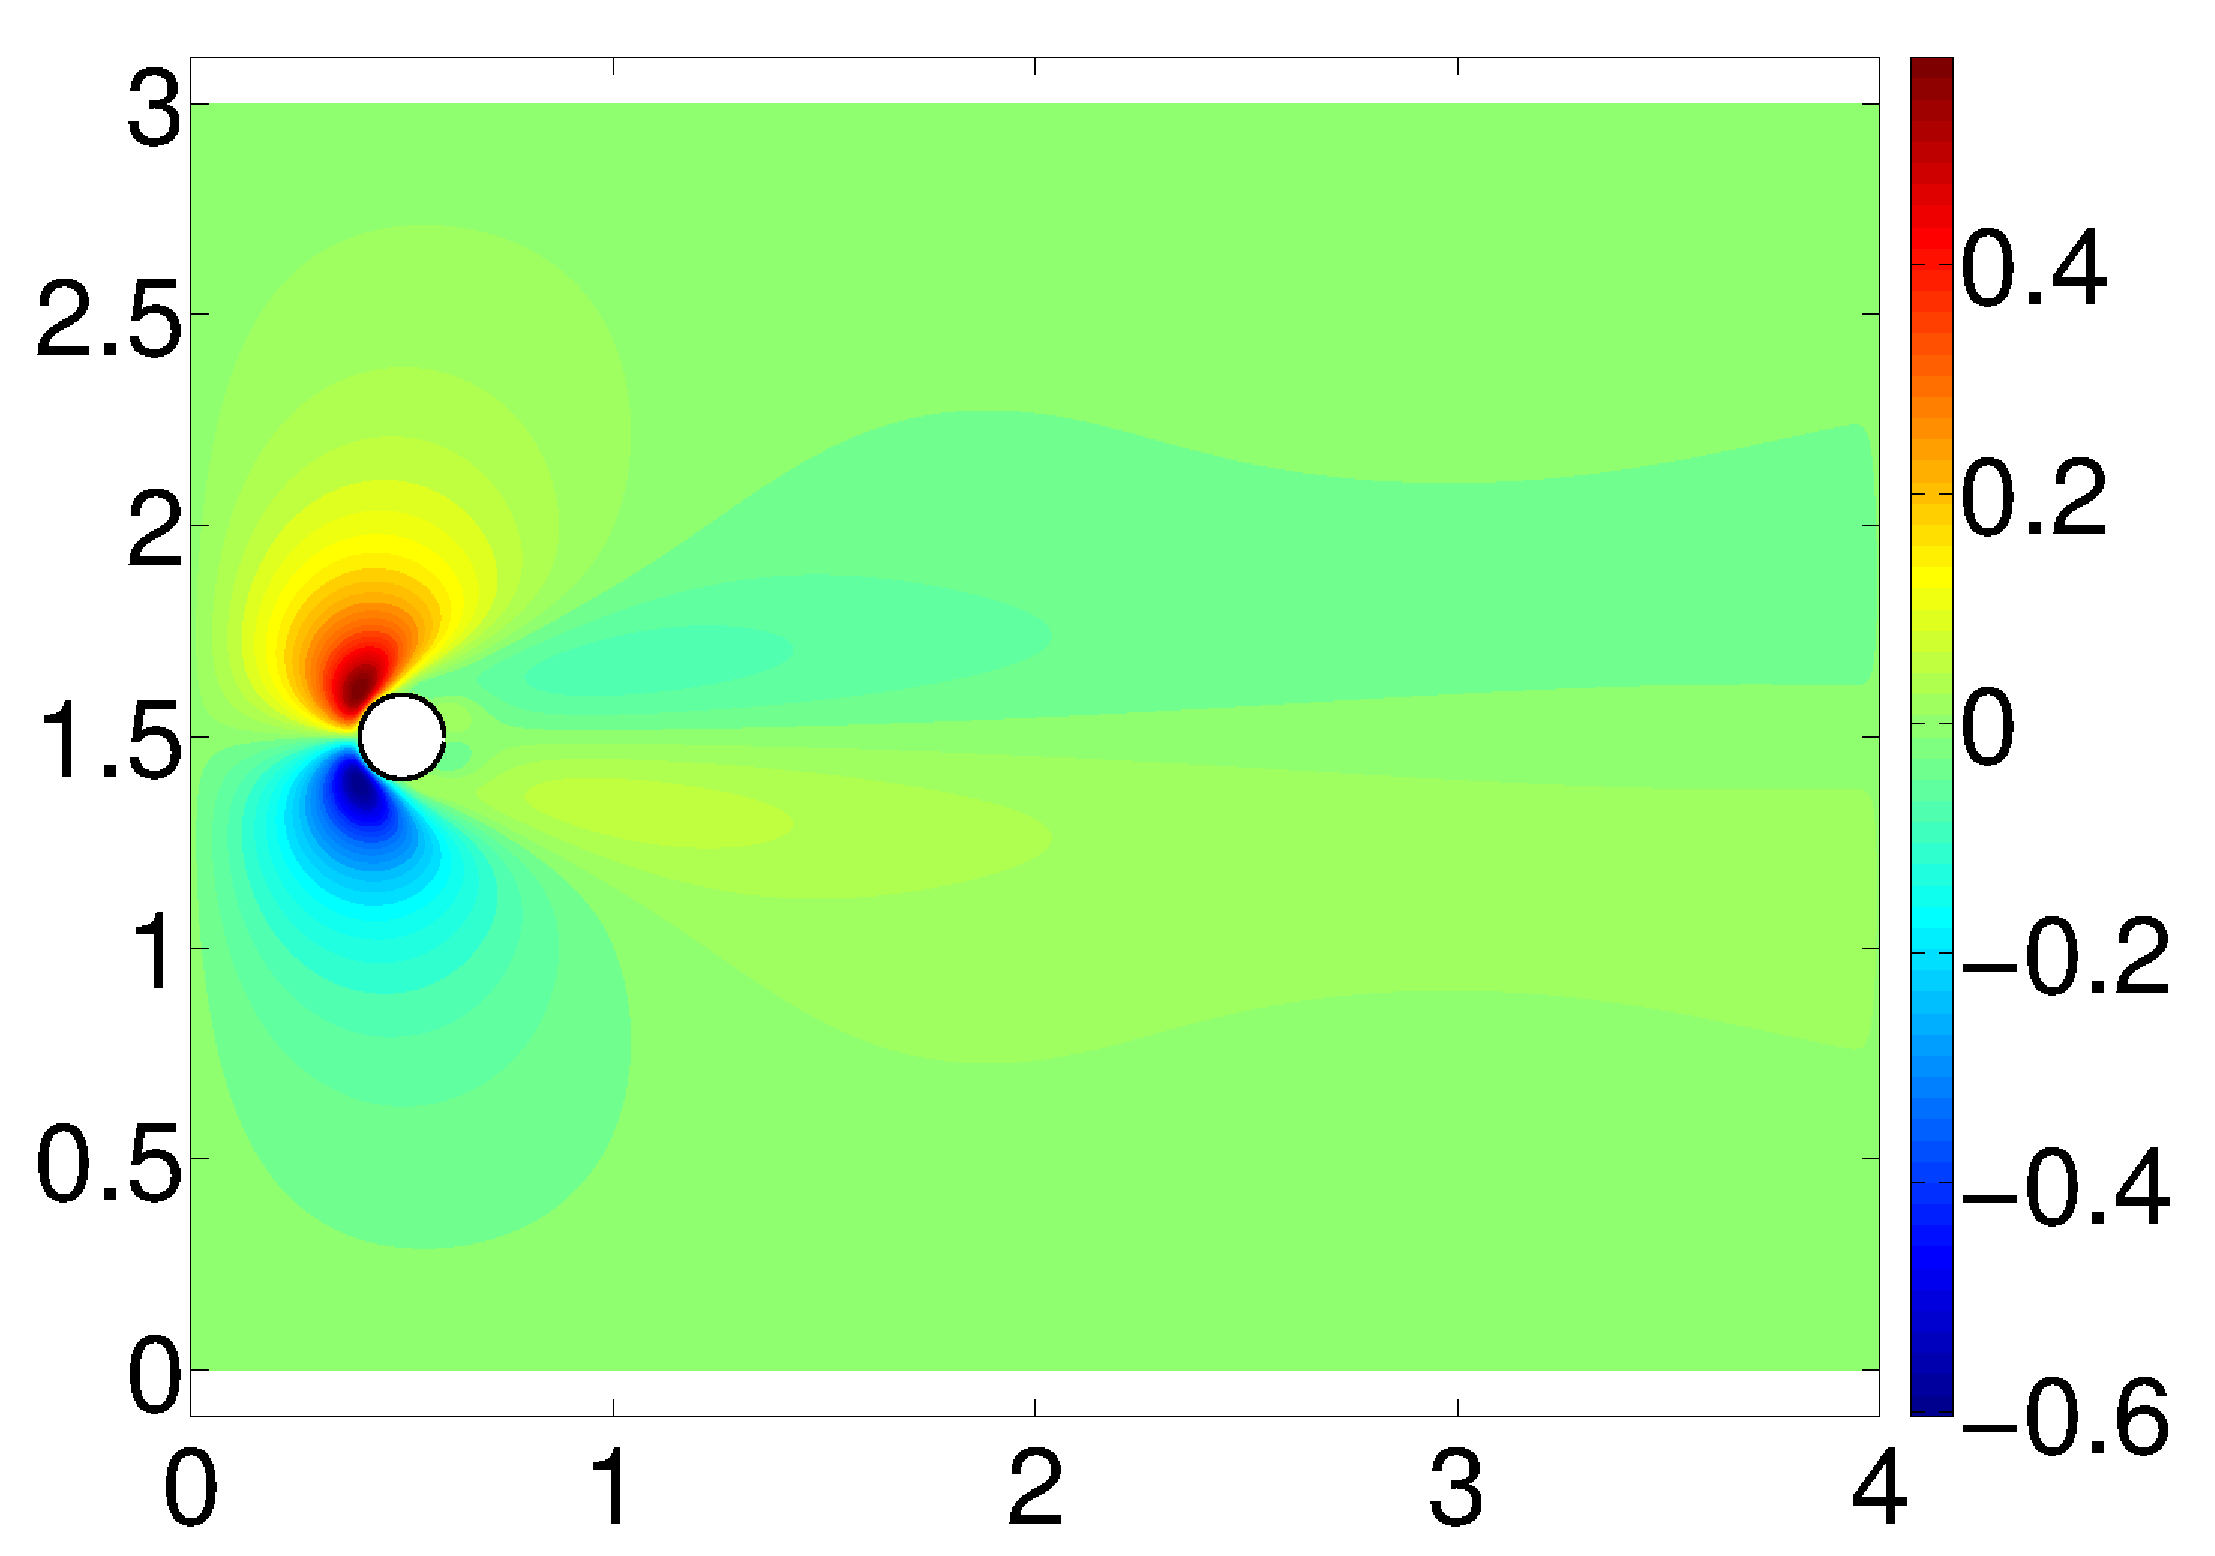
\includegraphics[width=6.5cm]{Chapter_4/figure/flow_over_cylinder/v_velocity_contour_RE100.eps}
    }
    \\
    \subfigure[Pressure]
    {
    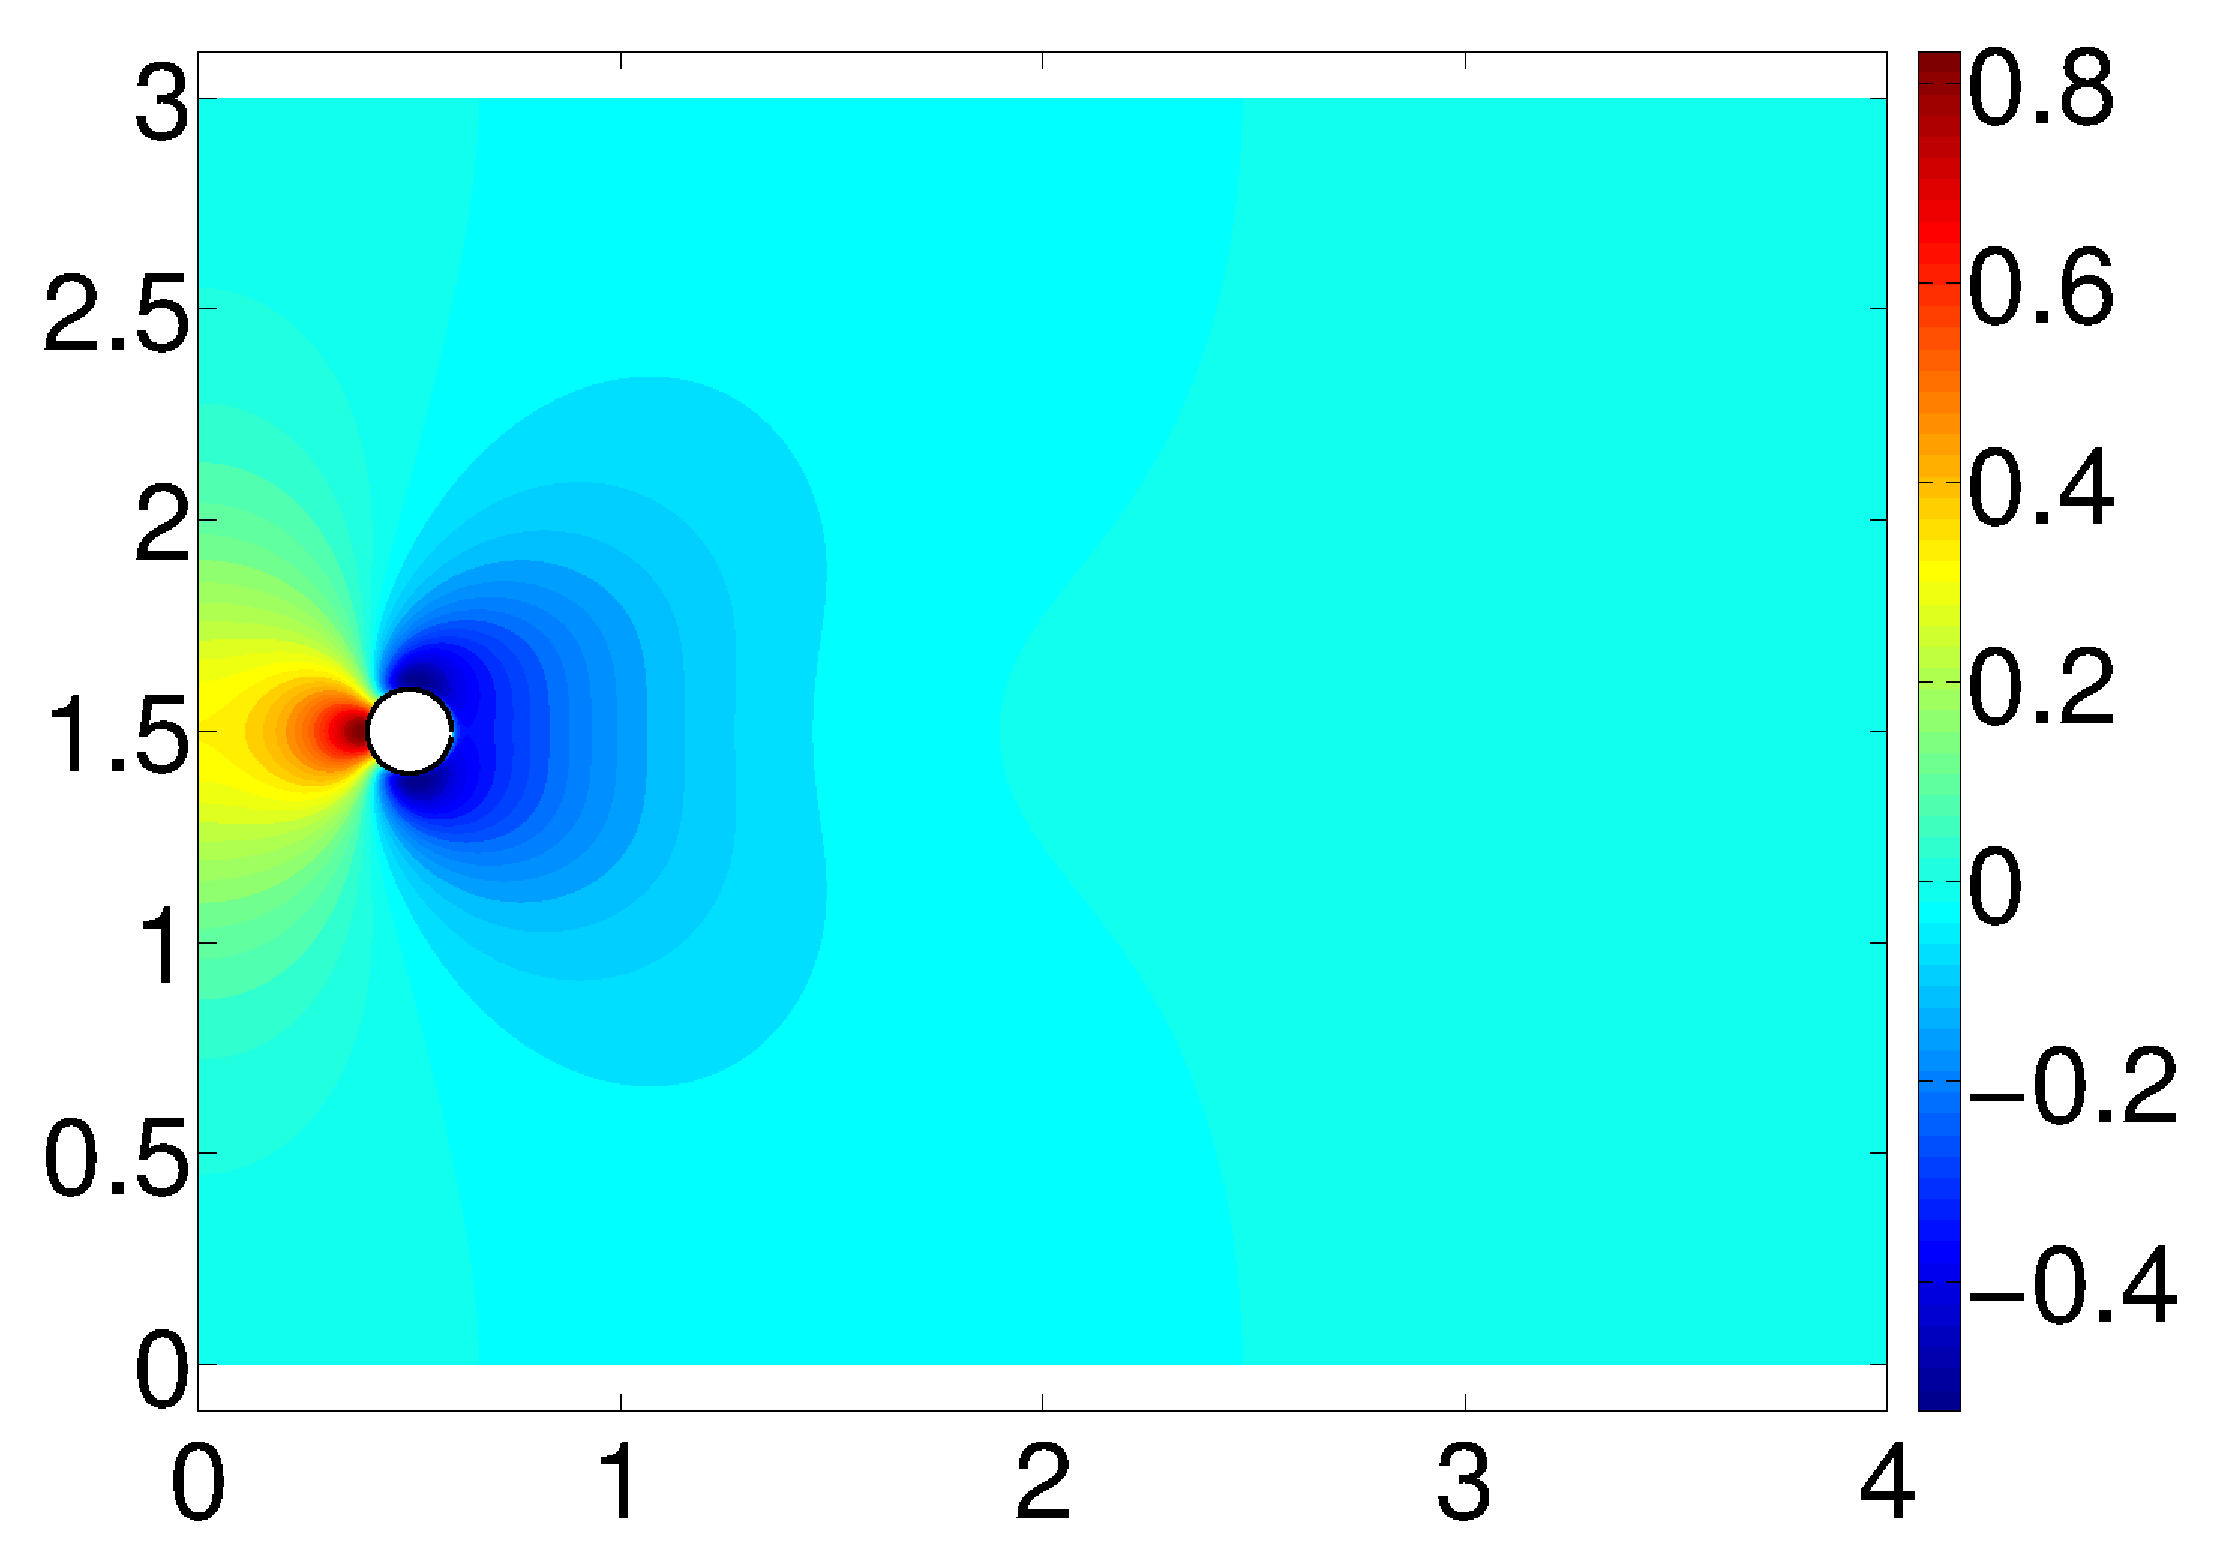
\includegraphics[width=6.5cm]{Chapter_4/figure/flow_over_cylinder/pressure_contour_RE100.eps}
    }
    \caption{Velocity and pressure contours for Re = 100.}
    \label{fig:C4_contourPlotsForFlowOverCylidnerGE}
\end{figure}
%
To ensure zero velocity on the solid boundary, we looked at the value of $u$ and $v$ velocities at the Lagrangian points on the boundary. These are shown in Figure \ref{fig:C4_fluidVelocityOnCylinder}. As shown here, the forcing terms brought the velocity to zero within the accuracy requirement. $\theta$ is the polar coordinate of Lagrangian points on the cylinder surface as shown in Figure \ref{fig:C4_cylinderPhysicalDomain}.
%
\begin{figure}[H]
    \centering
    \subfigure[U-velocity]
    {
    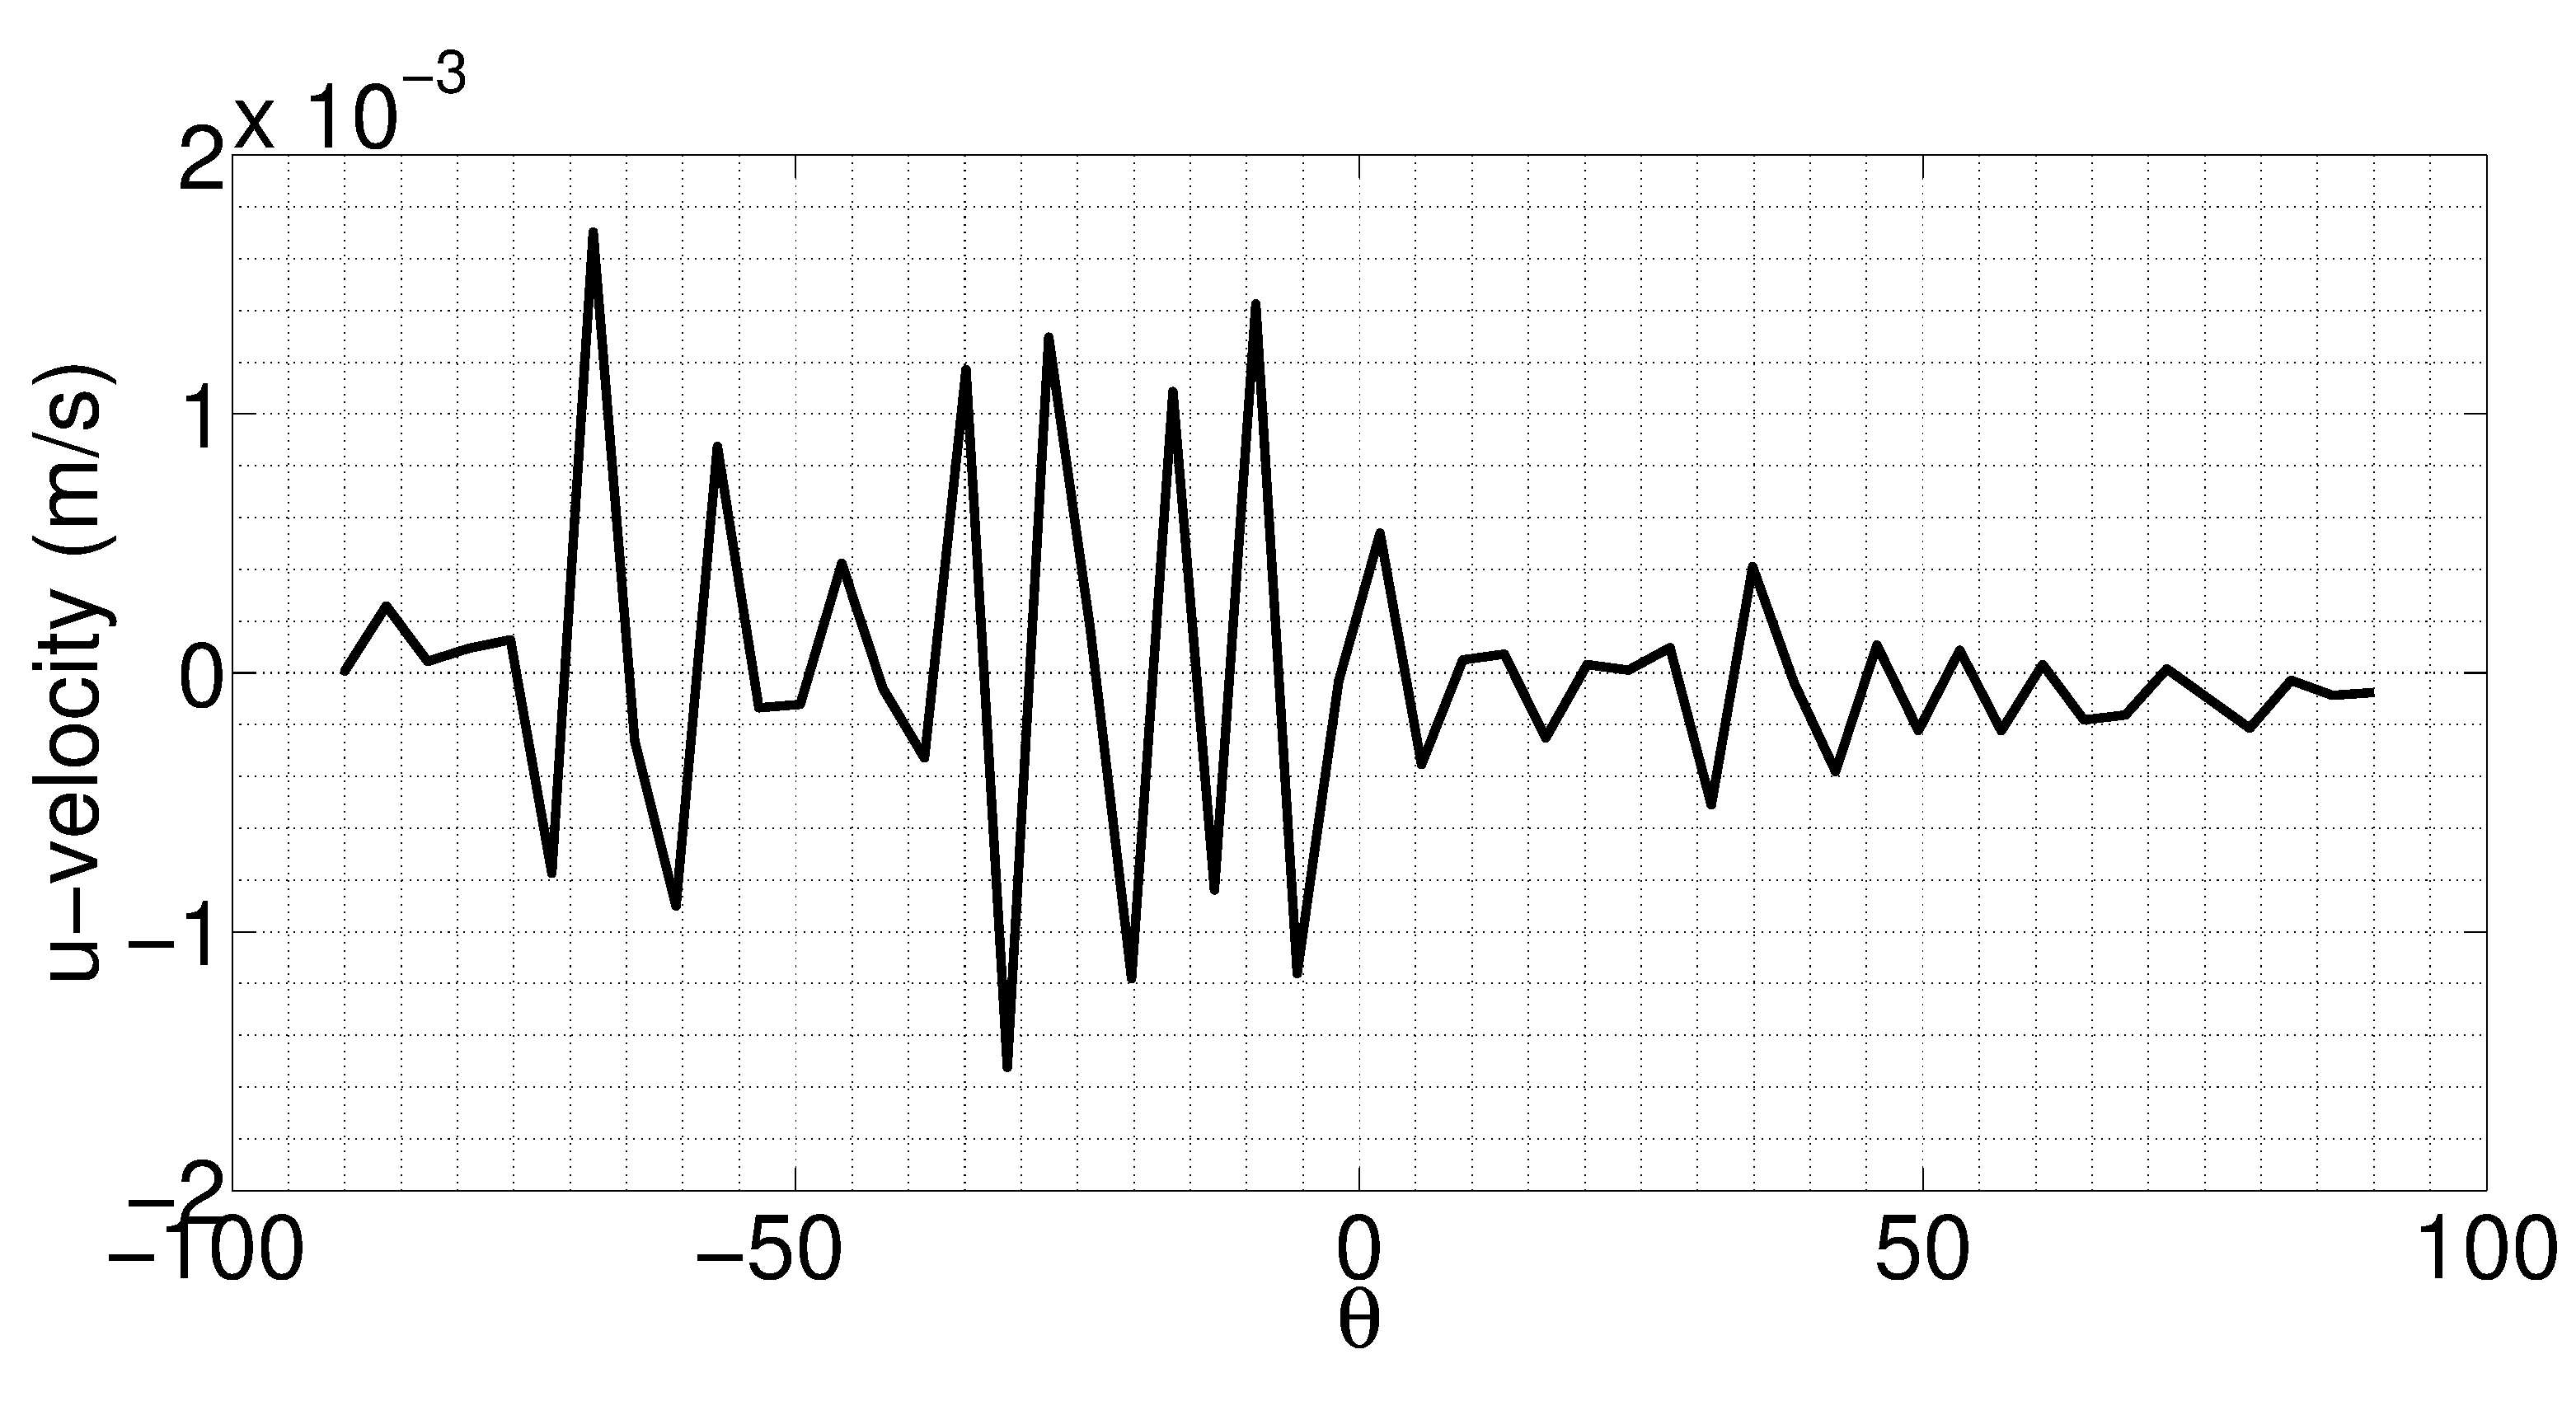
\includegraphics[width=6.5cm]{Chapter_4/figure/flow_over_cylinder/u_on_boundary_RE100.eps}
    }
    \quad
    \subfigure[V-velocity]
    {
    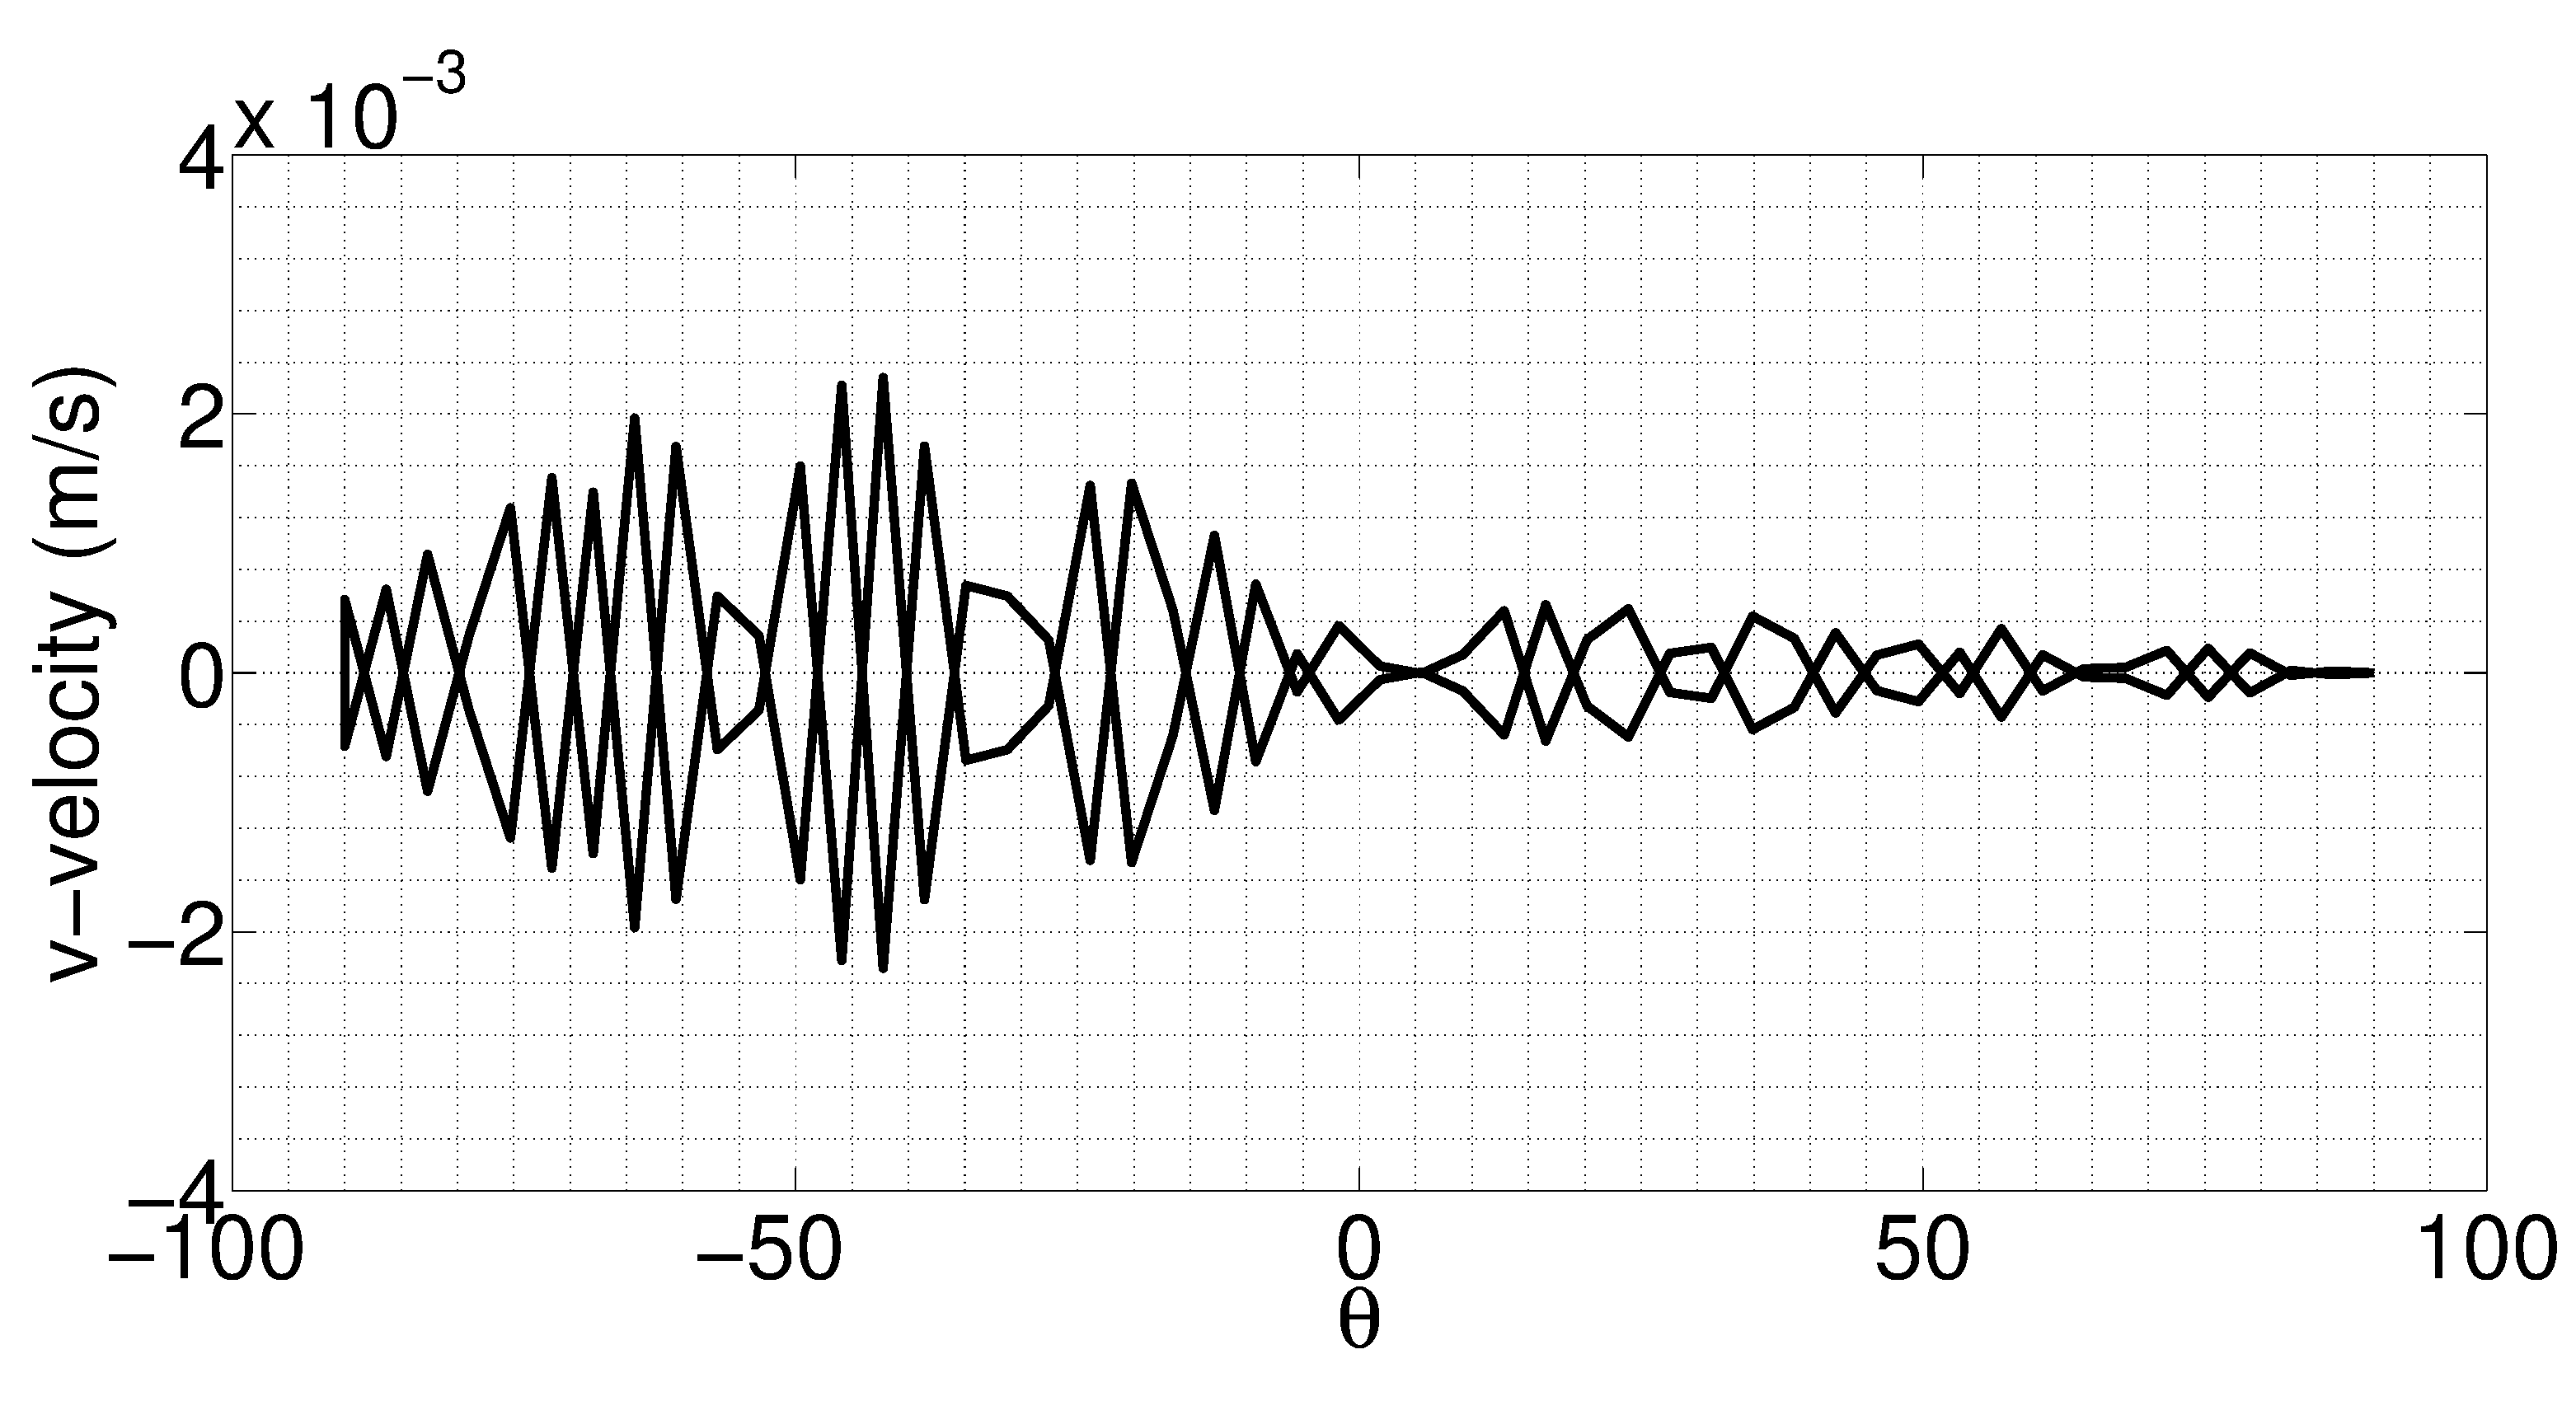
\includegraphics[width=6.5cm]{Chapter_4/figure/flow_over_cylinder/v_on_boundary_RE100.eps}
    }
    \caption{Velocity components on the solid boundary for Re = 100.}
    \label{fig:C4_fluidVelocityOnCylinder}
\end{figure}
%
Finally, the pressure profile on the cylinder surface is calculated as shown in Figure \ref{fig:C4_pressureOnSurfaceCylinder}. No smoothing is done for calculating the pressure values at the Lagrangian points. This data is interpolated using the RD function of Equation \eqref{eq:C4_deltaFunction}. As shown here, the pressure distribution on the boundary is smooth. This is in contrast to other IB methods that result in a non-smooth pressure profiles over the boundaries.
%
\begin{figure}[H]
    \centering
    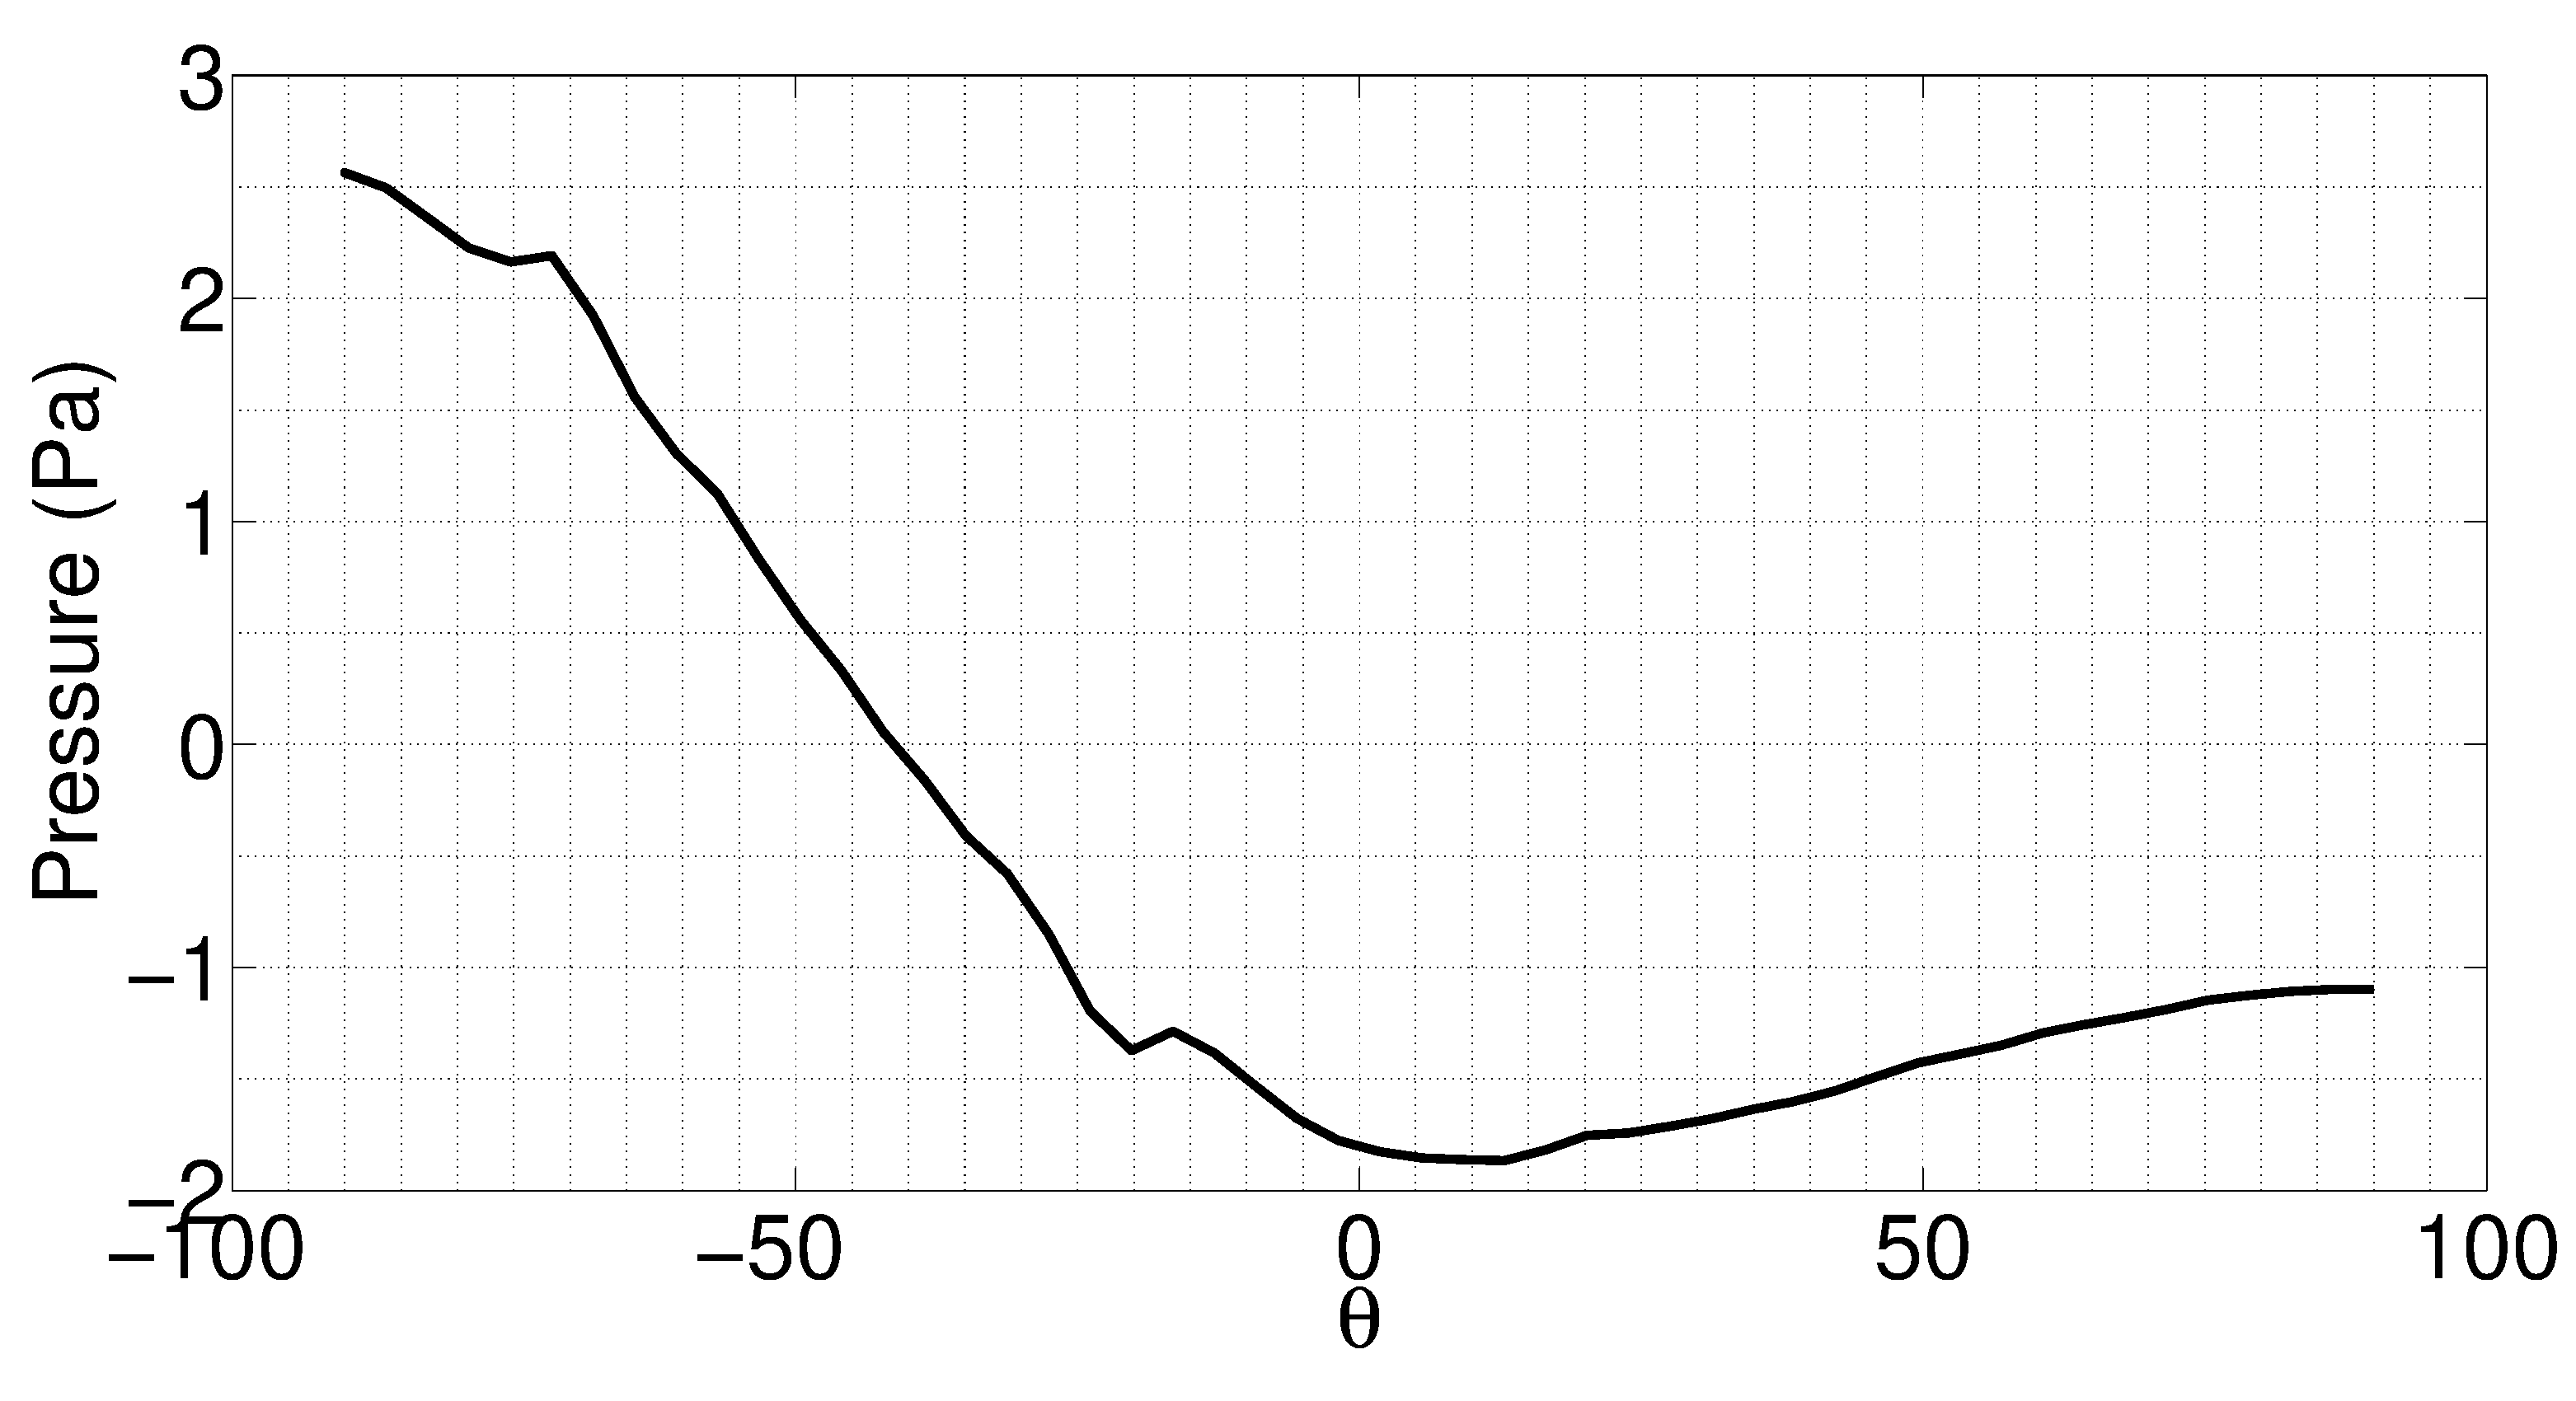
\includegraphics[width=12.00cm]{Chapter_4/figure/flow_over_cylinder/p_on_boundary_RE100.eps}
    \caption{Physical domain with dimensions for flow over cylinder.}
    \label{fig:C4_pressureOnSurfaceCylinder}
\end{figure}
%
The continuum sensitivity equations are derived by differentiating the governing NS equations of \eqref{eq:C4_NSwithvirtualBoundaryIB} with respect to the shape design variable, $b$, as shown in Equation \eqref{eq:C4_NSwithvirtualBoundaryIBsensitivity}. For this problem, the cylinder boundary is defined using the following analytical level-set function. For the points on the cylinder surface, Equation \eqref{eq:C4_levelSetFunctionForCylinder} holds.
%
\begin{equation}\label{eq:C4_levelSetFunctionForCylinder}
	\mathcal{R}(x, y; r): (x - x_0)^2 + (y - y_0)^2 = r^2
\end{equation}
%
For the sensitivity analysis, $\partial D/\partial X$ is calculated easily, since the analytical form of the RD function is known (Equation \eqref{eq:C4_deltaFunction}). It is possible to calculate the $\partial X/\partial b$ values in Equation \eqref{eq:C4_NSwithvirtualBoundaryIBsensitivity} by differentiating Equation \eqref{eq:C4_levelSetFunctionForCylinder}. This is done in Equation \eqref{eq:C4_levelSetFunctionForCylinderSA}.
%
\begin{equation}\label{eq:C4_levelSetFunctionForCylinderSA}
	\frac{\partial \mathcal{R}(x, y; r)}{\partial b}: 
	2 (x - x_0)\dfrac{\partial x}{\partial b} + 
	2 (y - y_0)\frac{\partial y}{\partial b} = 
	2 r \frac{\partial r}{\partial b}
\end{equation}
%
For this analysis, the design variable, $b$, is selected as the radius of the cylinder; therefore, the right-hand-side of Equation \eqref{eq:C4_levelSetFunctionForCylinderSA} reduces to $2r$.

The boundary conditions for the sensitivity analysis are defined by differentiating the original boundary conditions of the governing equations. These conditions do not depend on the design variables and therefore their material derivatives have zero values. These conditions are applied using a fourth order approximation on the far field boundaries of sensitivity equation. It should be noted that the solver uses second order discretization for the boundary condition. This is required for accurate sensitivity calculation. Obtaining the differentiated governing equations and boundary conditions, it is possible to solve the sensitivity equations.

The complex step method is used to validate the sensitivity response of the system. As mentioned in Chapter \ref{ch:introduction}, the complex step method does not suffer from the accuracy issues of the finite difference method and provides the accurate sensitivities up to machine precision. However, the analysis code requires handling complex arithmetic. The analysis code is developed in MATLAB using the guidelines of \cite{martins2003complex} so that complex step can be used to calculate the sensitivities. The complex-step derivative is defined in Equation \eqref{eq:C1_compelxStepFormula}. The comparison of the CSA results with the complex step solution for the sensitivities of a different location in the domain is shown in Figure \ref{fig:C4_flowOverCylinderSensitivityValidation}. The RMSE value is used to compare the results of continuum sensitivity analysis (CSA) and complex step (CS) method. Figure \ref{fig:C4_flowOverCylinderSensitivityValidation} shows an acceptable comparison between the CSA and CS results.
%
\begin{figure}[H]
    \centering
    \subfigure[U-velocity sensitivity on $y = 1.50$]
    {
    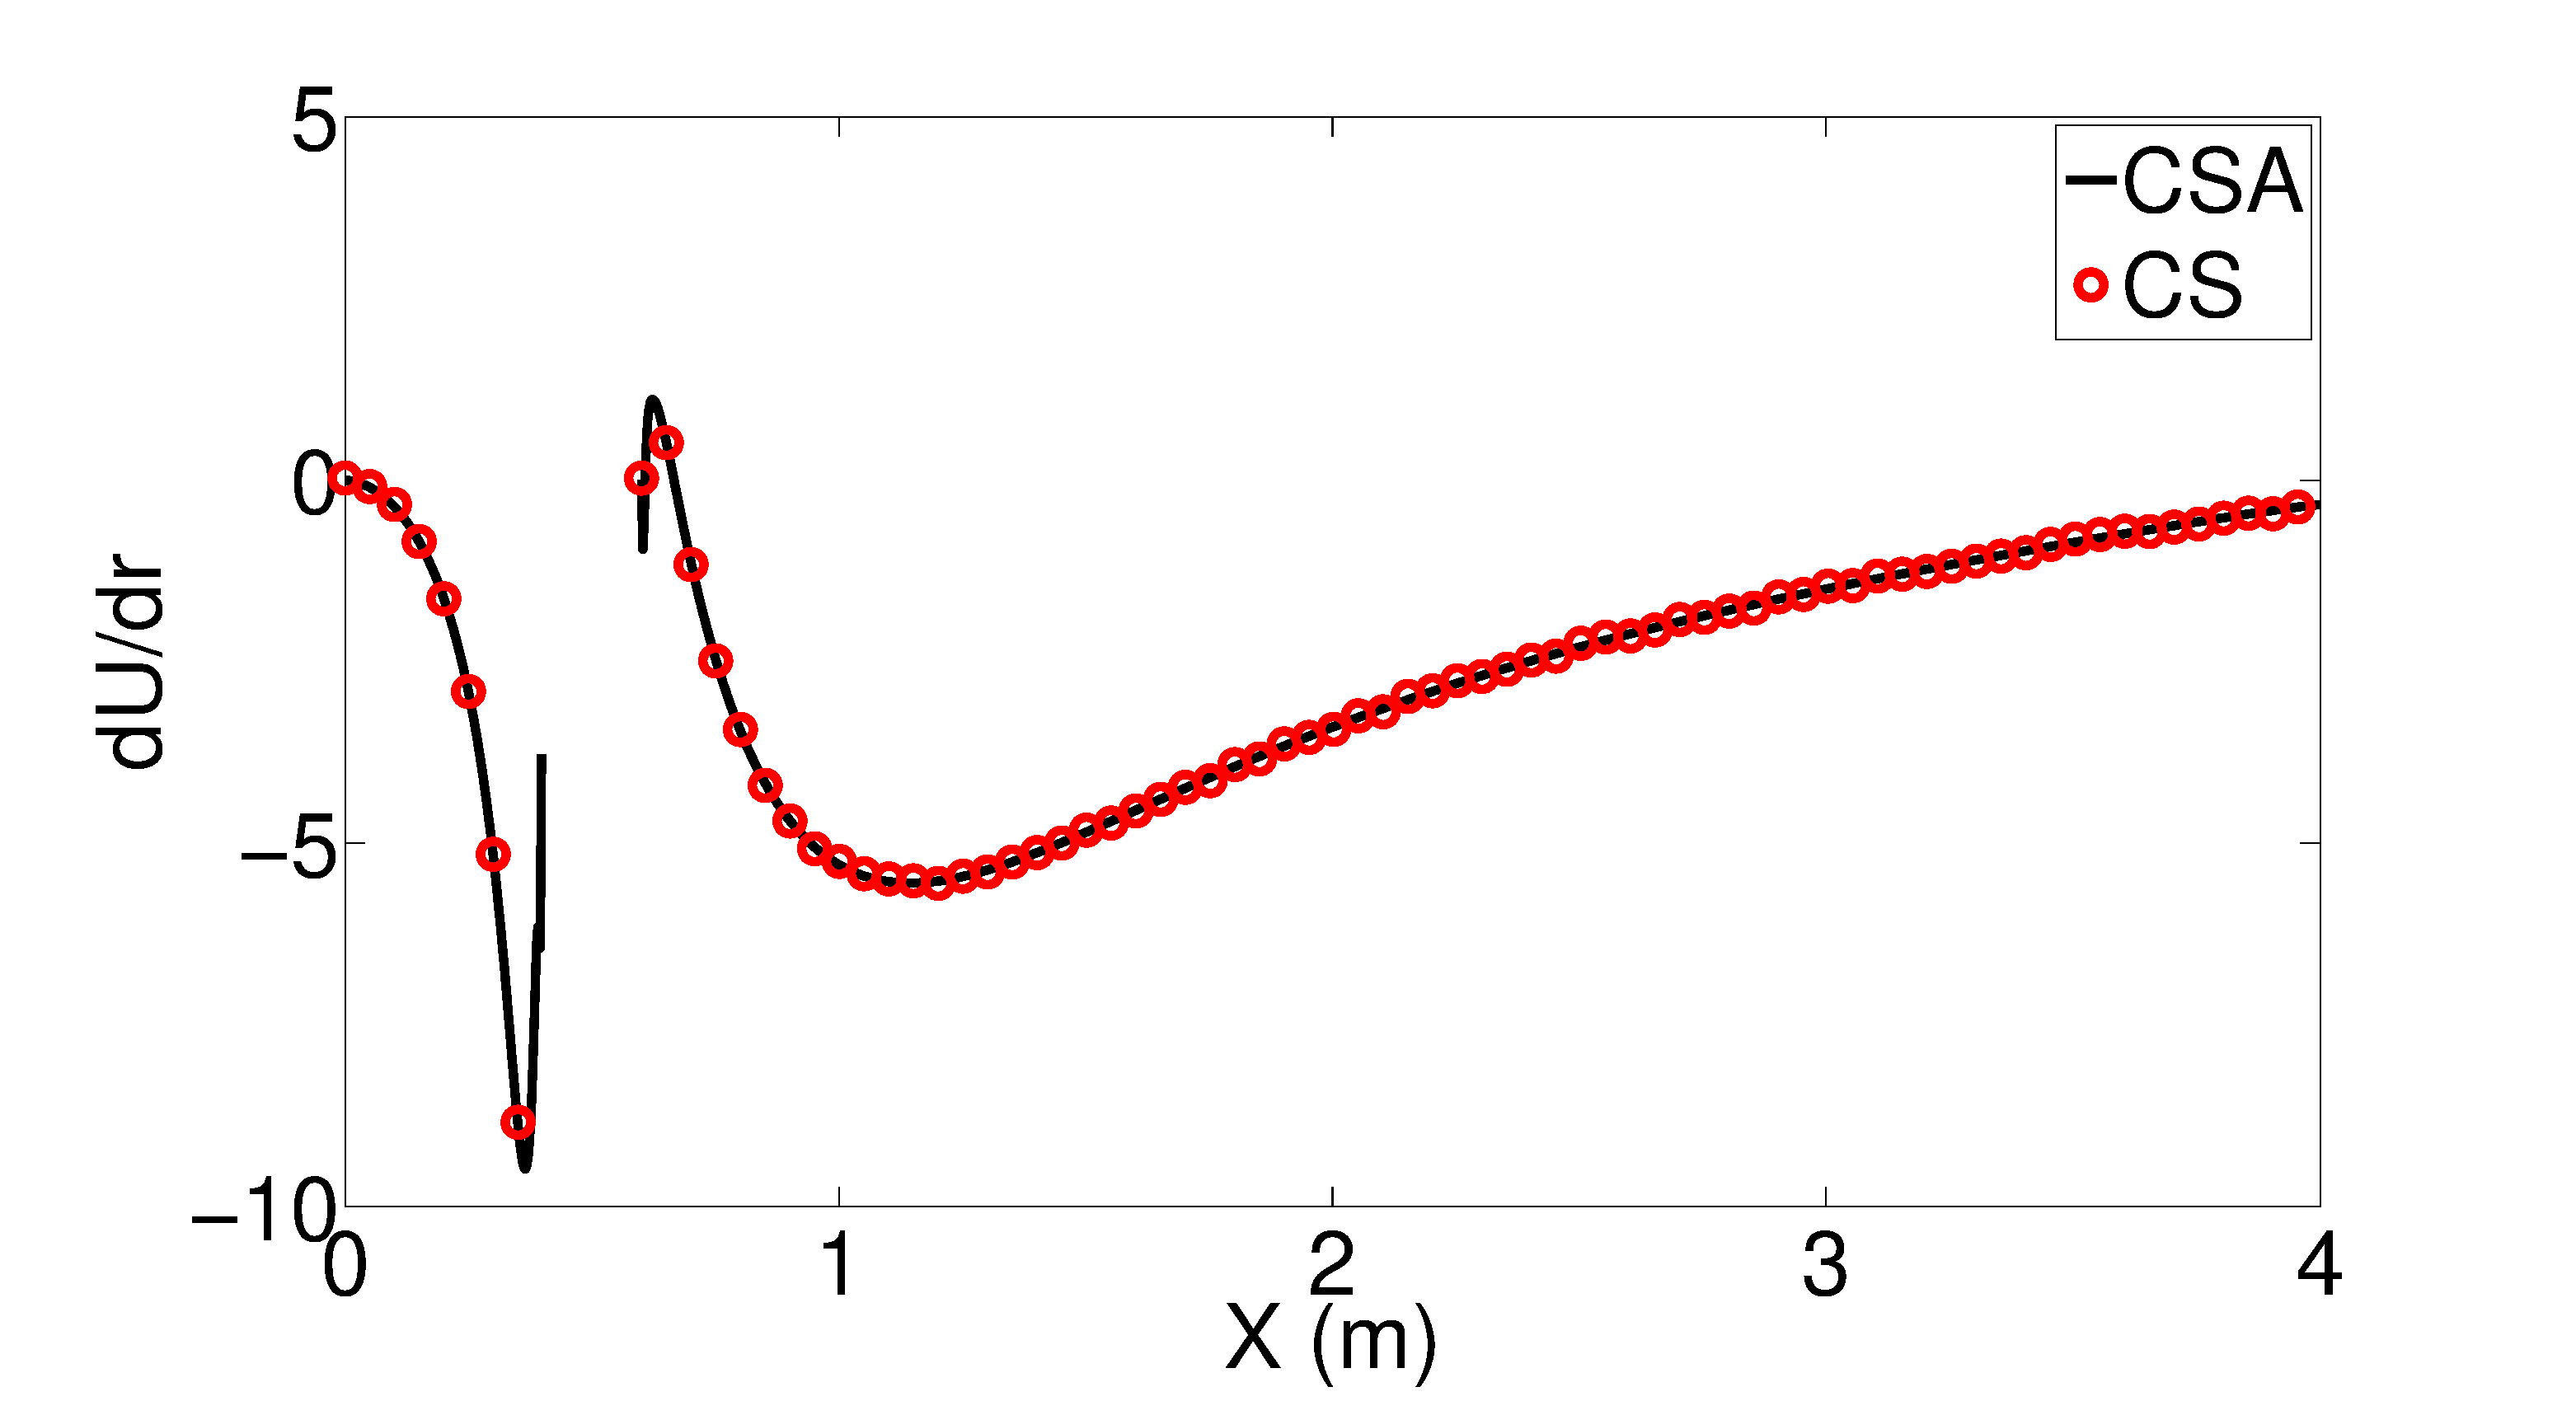
\includegraphics[width=6.5cm]{Chapter_4/figure/flow_over_cylinder/validation_dUdR_Y150_RE100.eps}
    }
    \quad
    \subfigure[U-velocity sensitivity on $x = 2.00$]
    {
    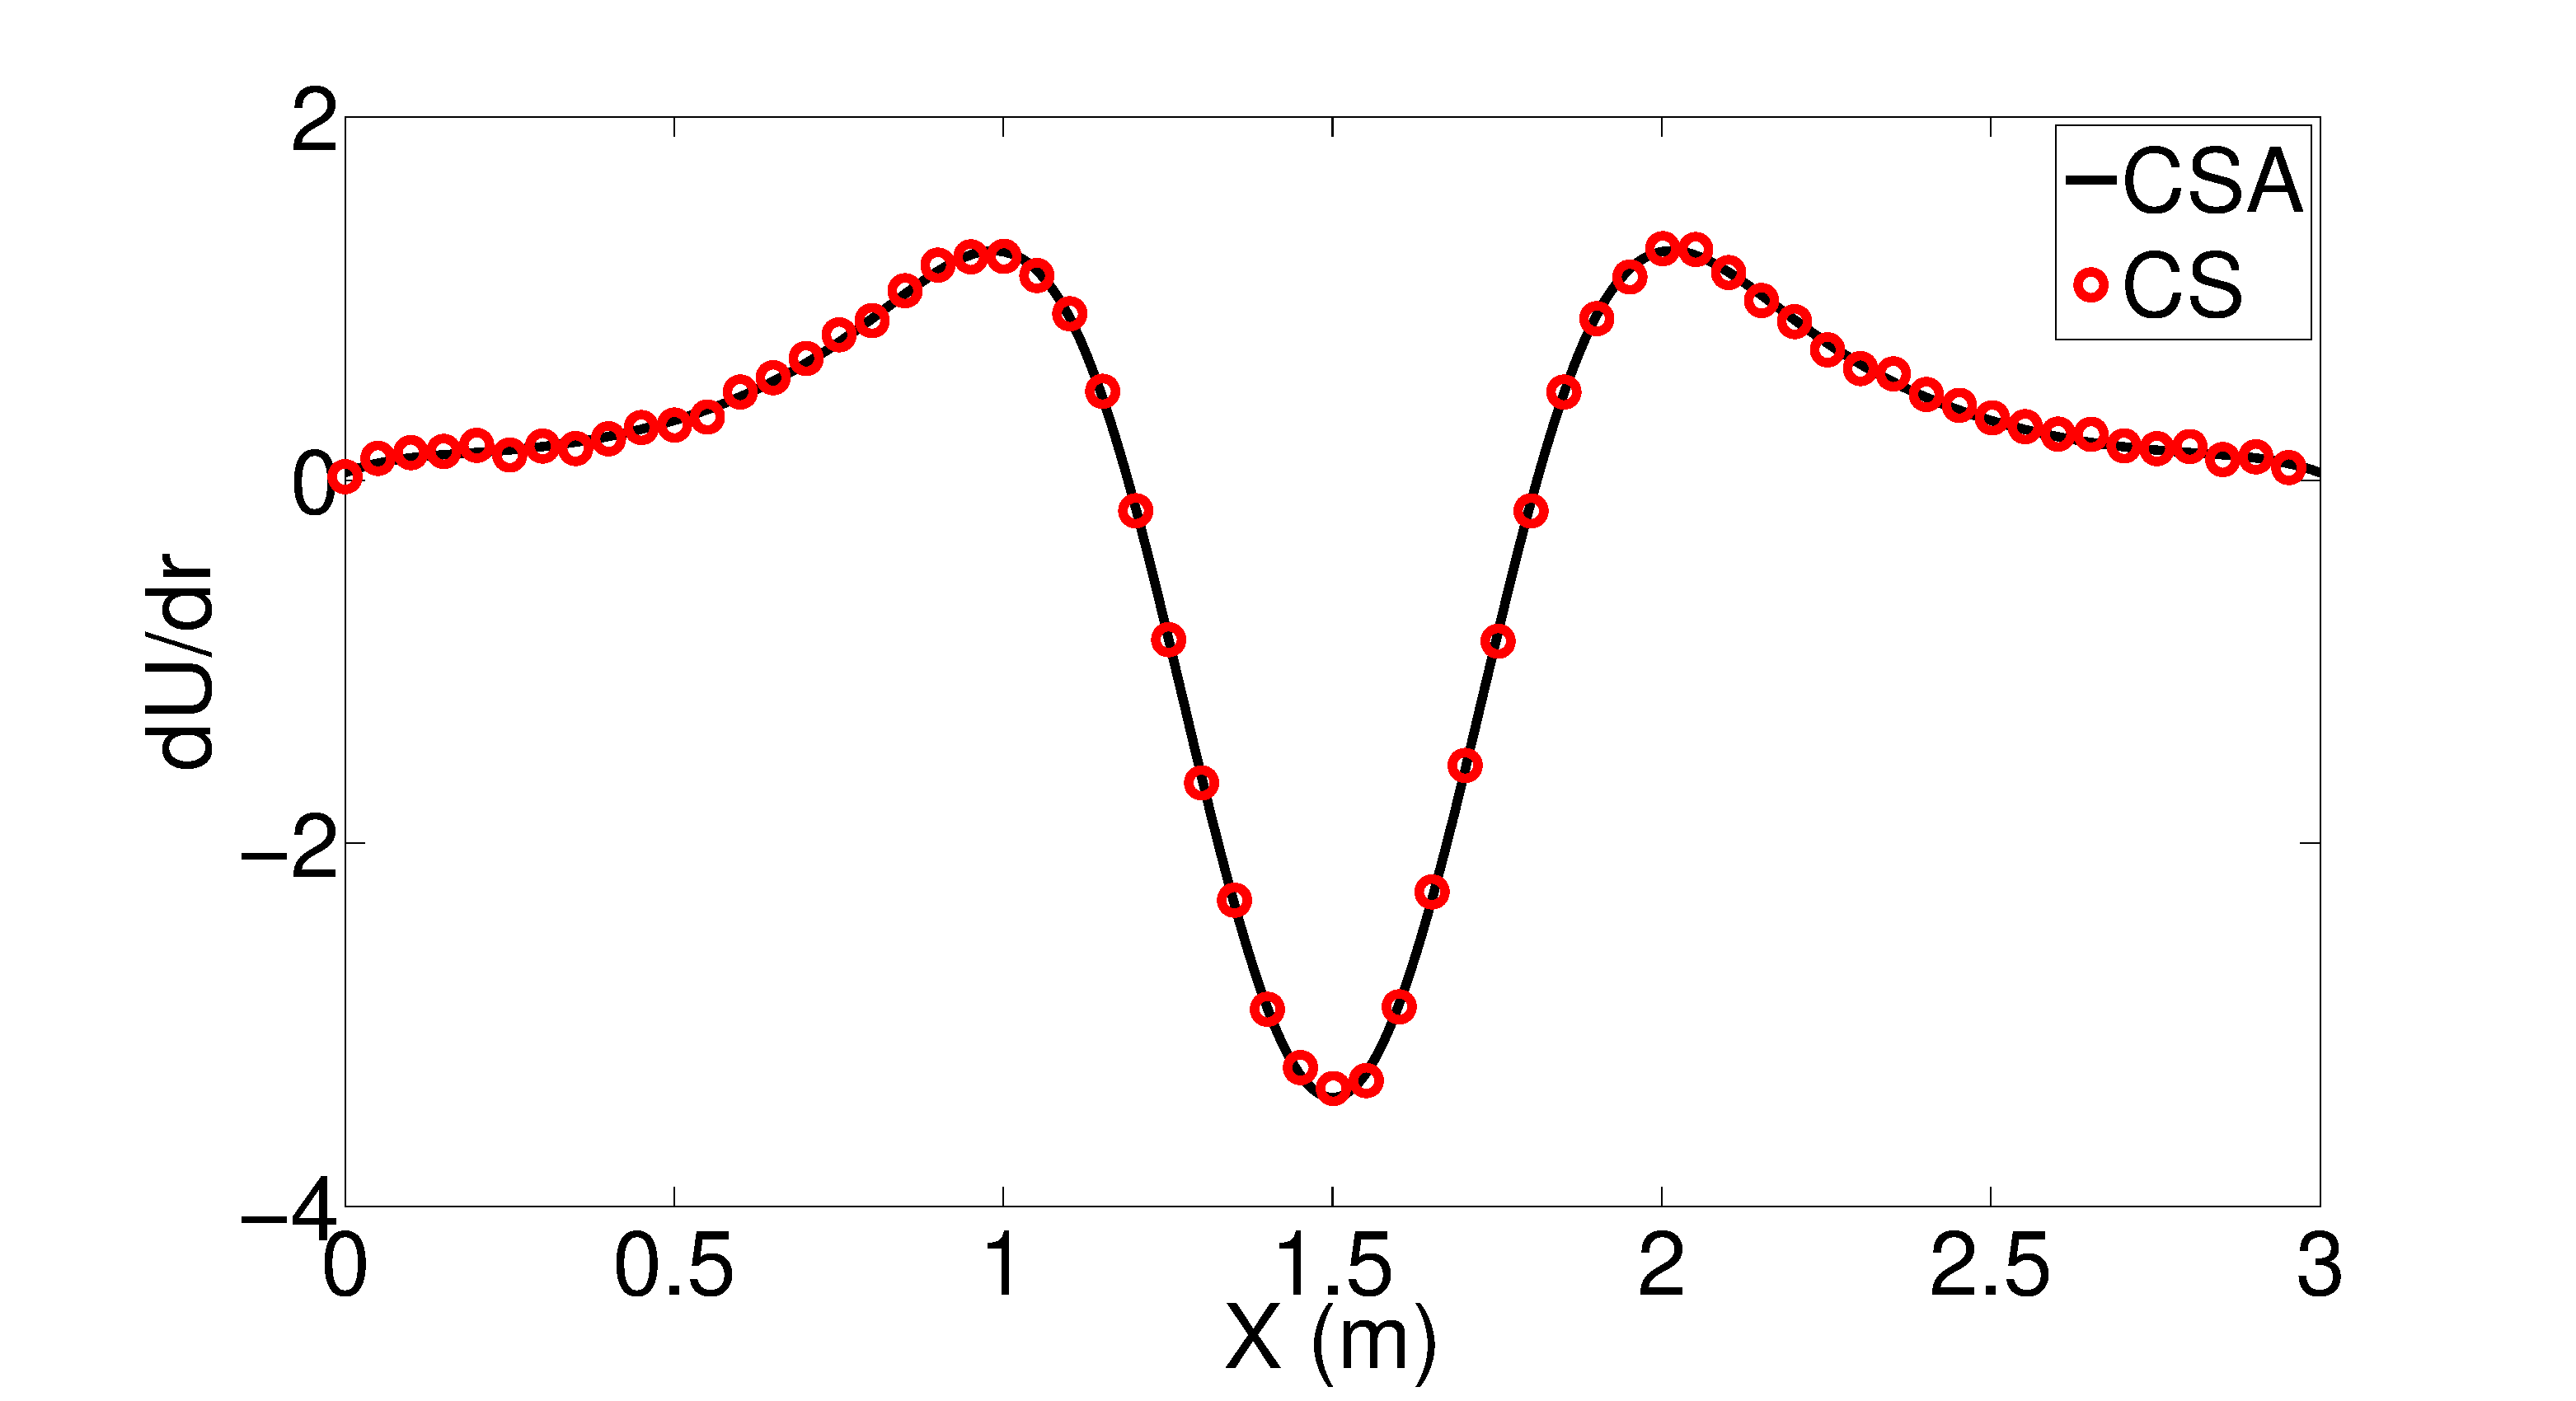
\includegraphics[width=6.5cm]{Chapter_4/figure/flow_over_cylinder/validation_dUdR_X200_RE100.eps}
    }
    \\
	\subfigure[V-velocity sensitivity on $y = 1.50$]
    {
    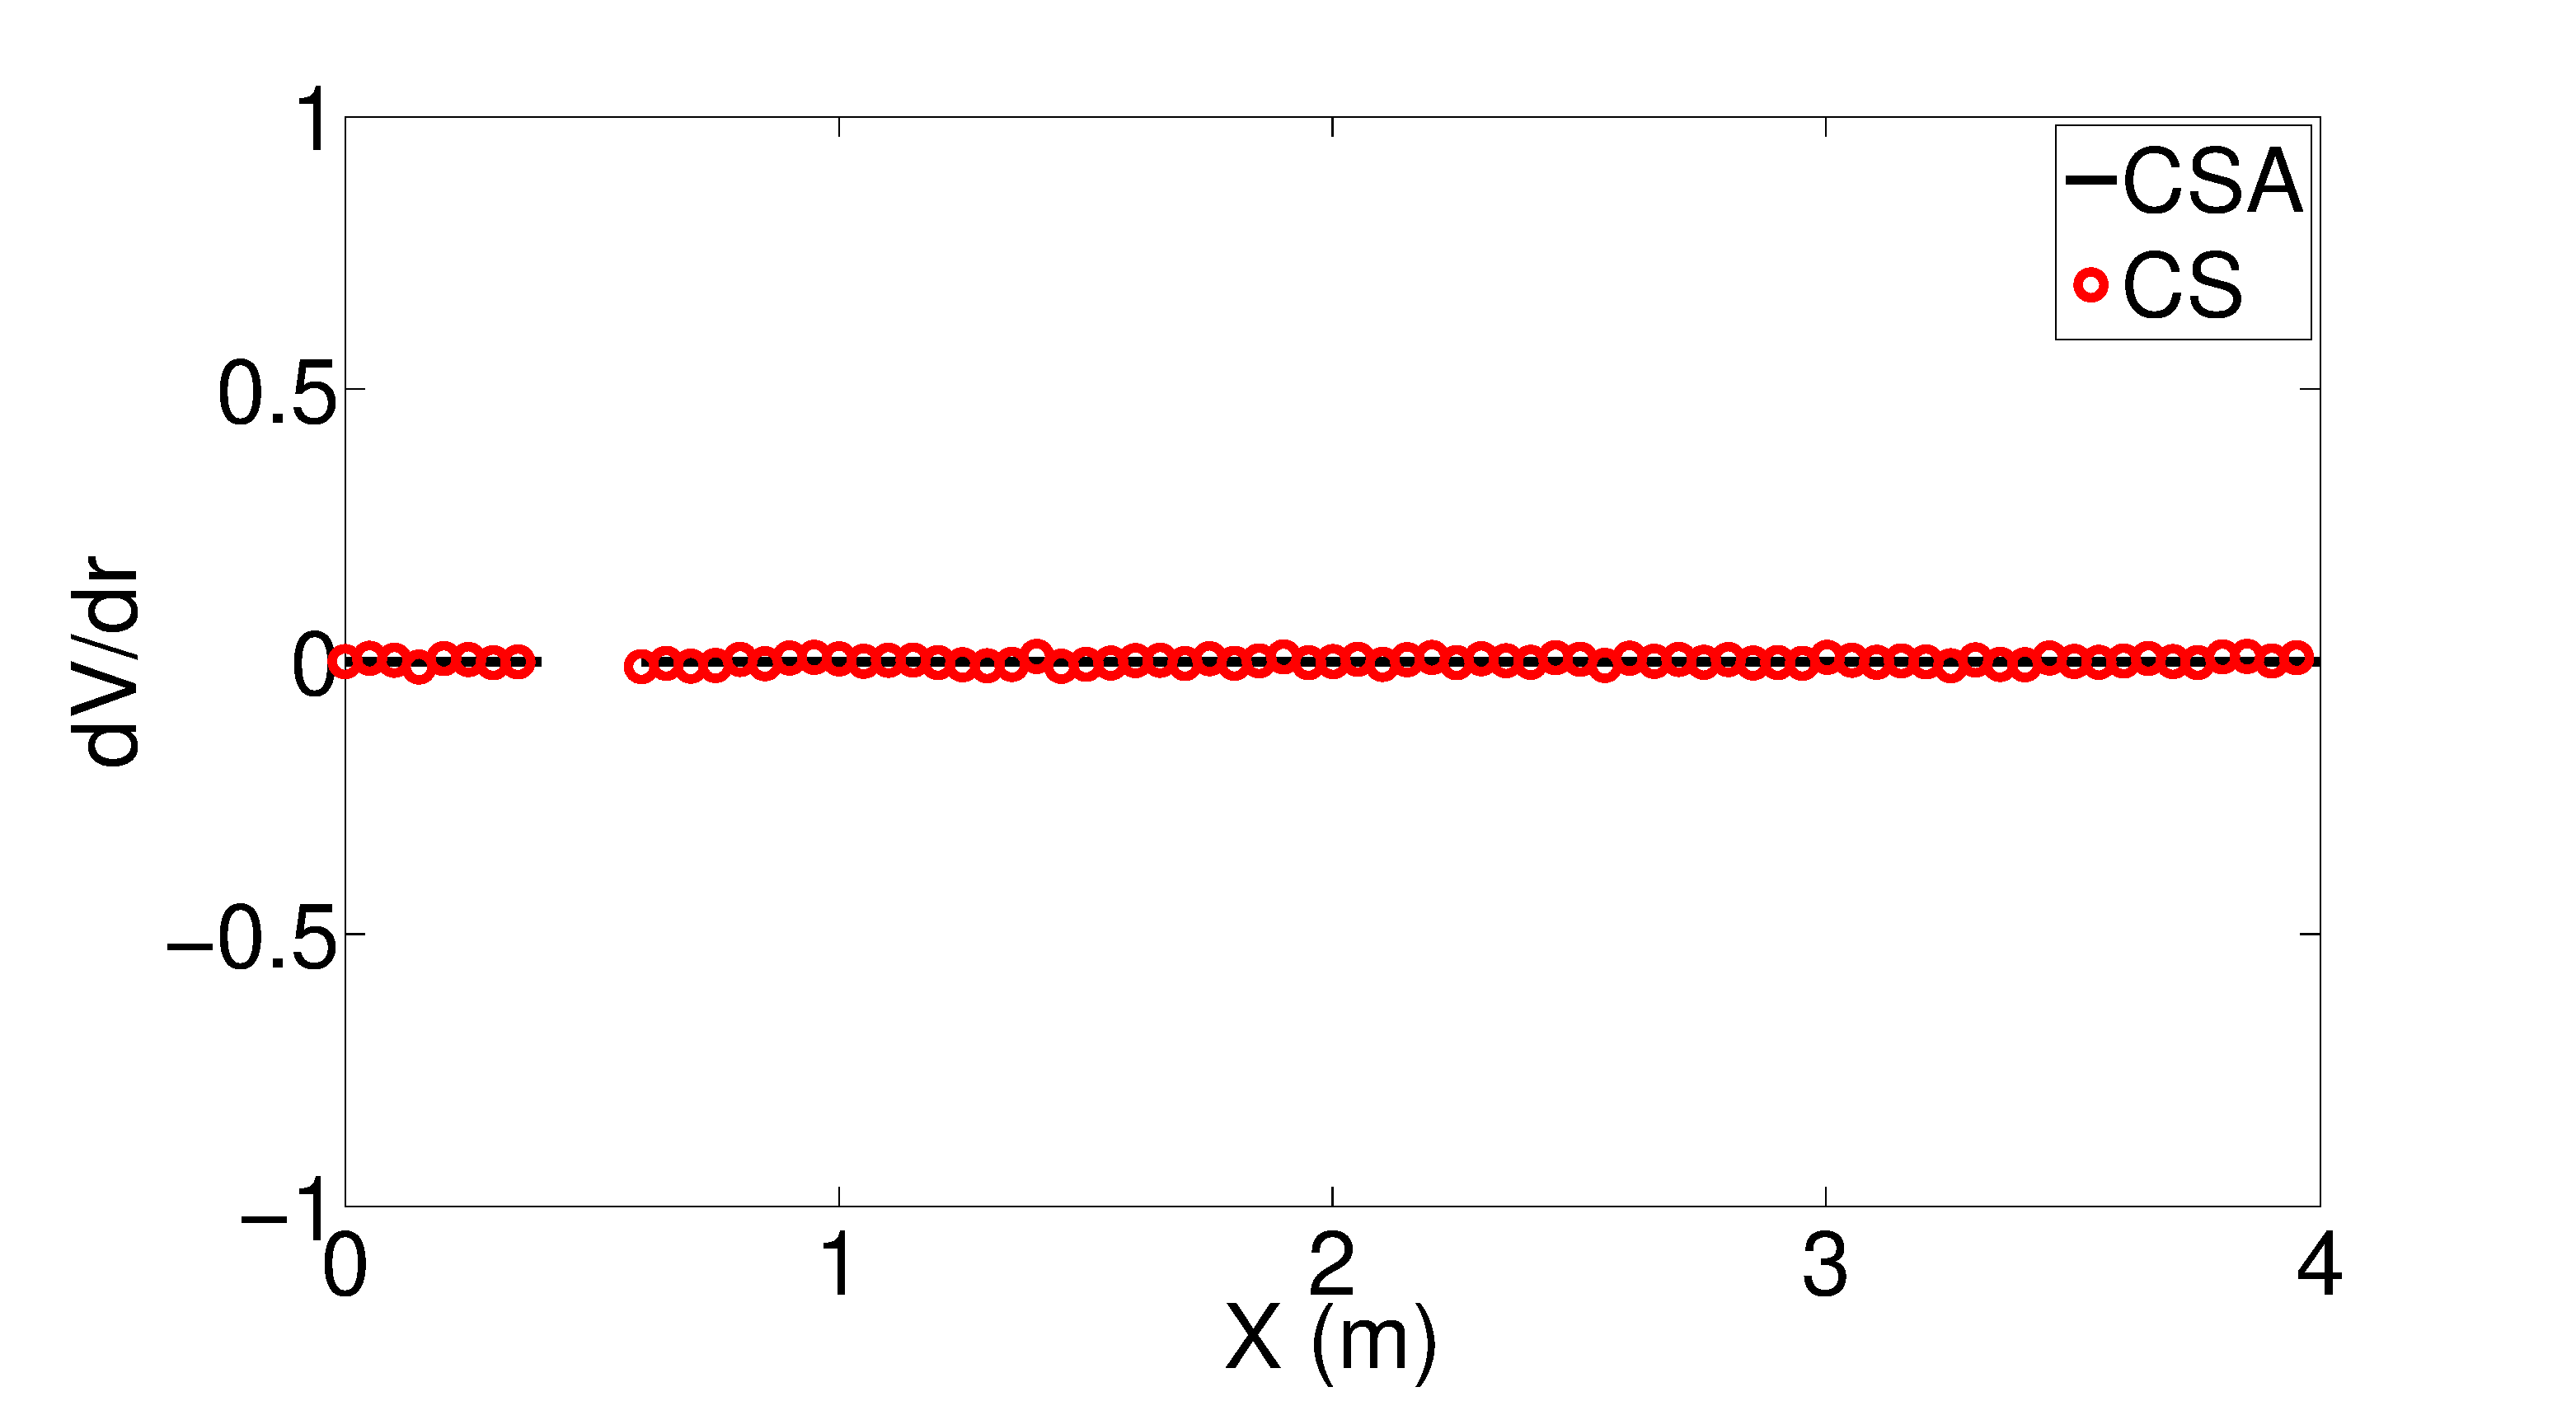
\includegraphics[width=6.5cm]{Chapter_4/figure/flow_over_cylinder/validation_dVdR_Y150_RE100.eps}
    }
    \quad
    \subfigure[V-velocity sensitivity on $x = 2.00$]
    {
    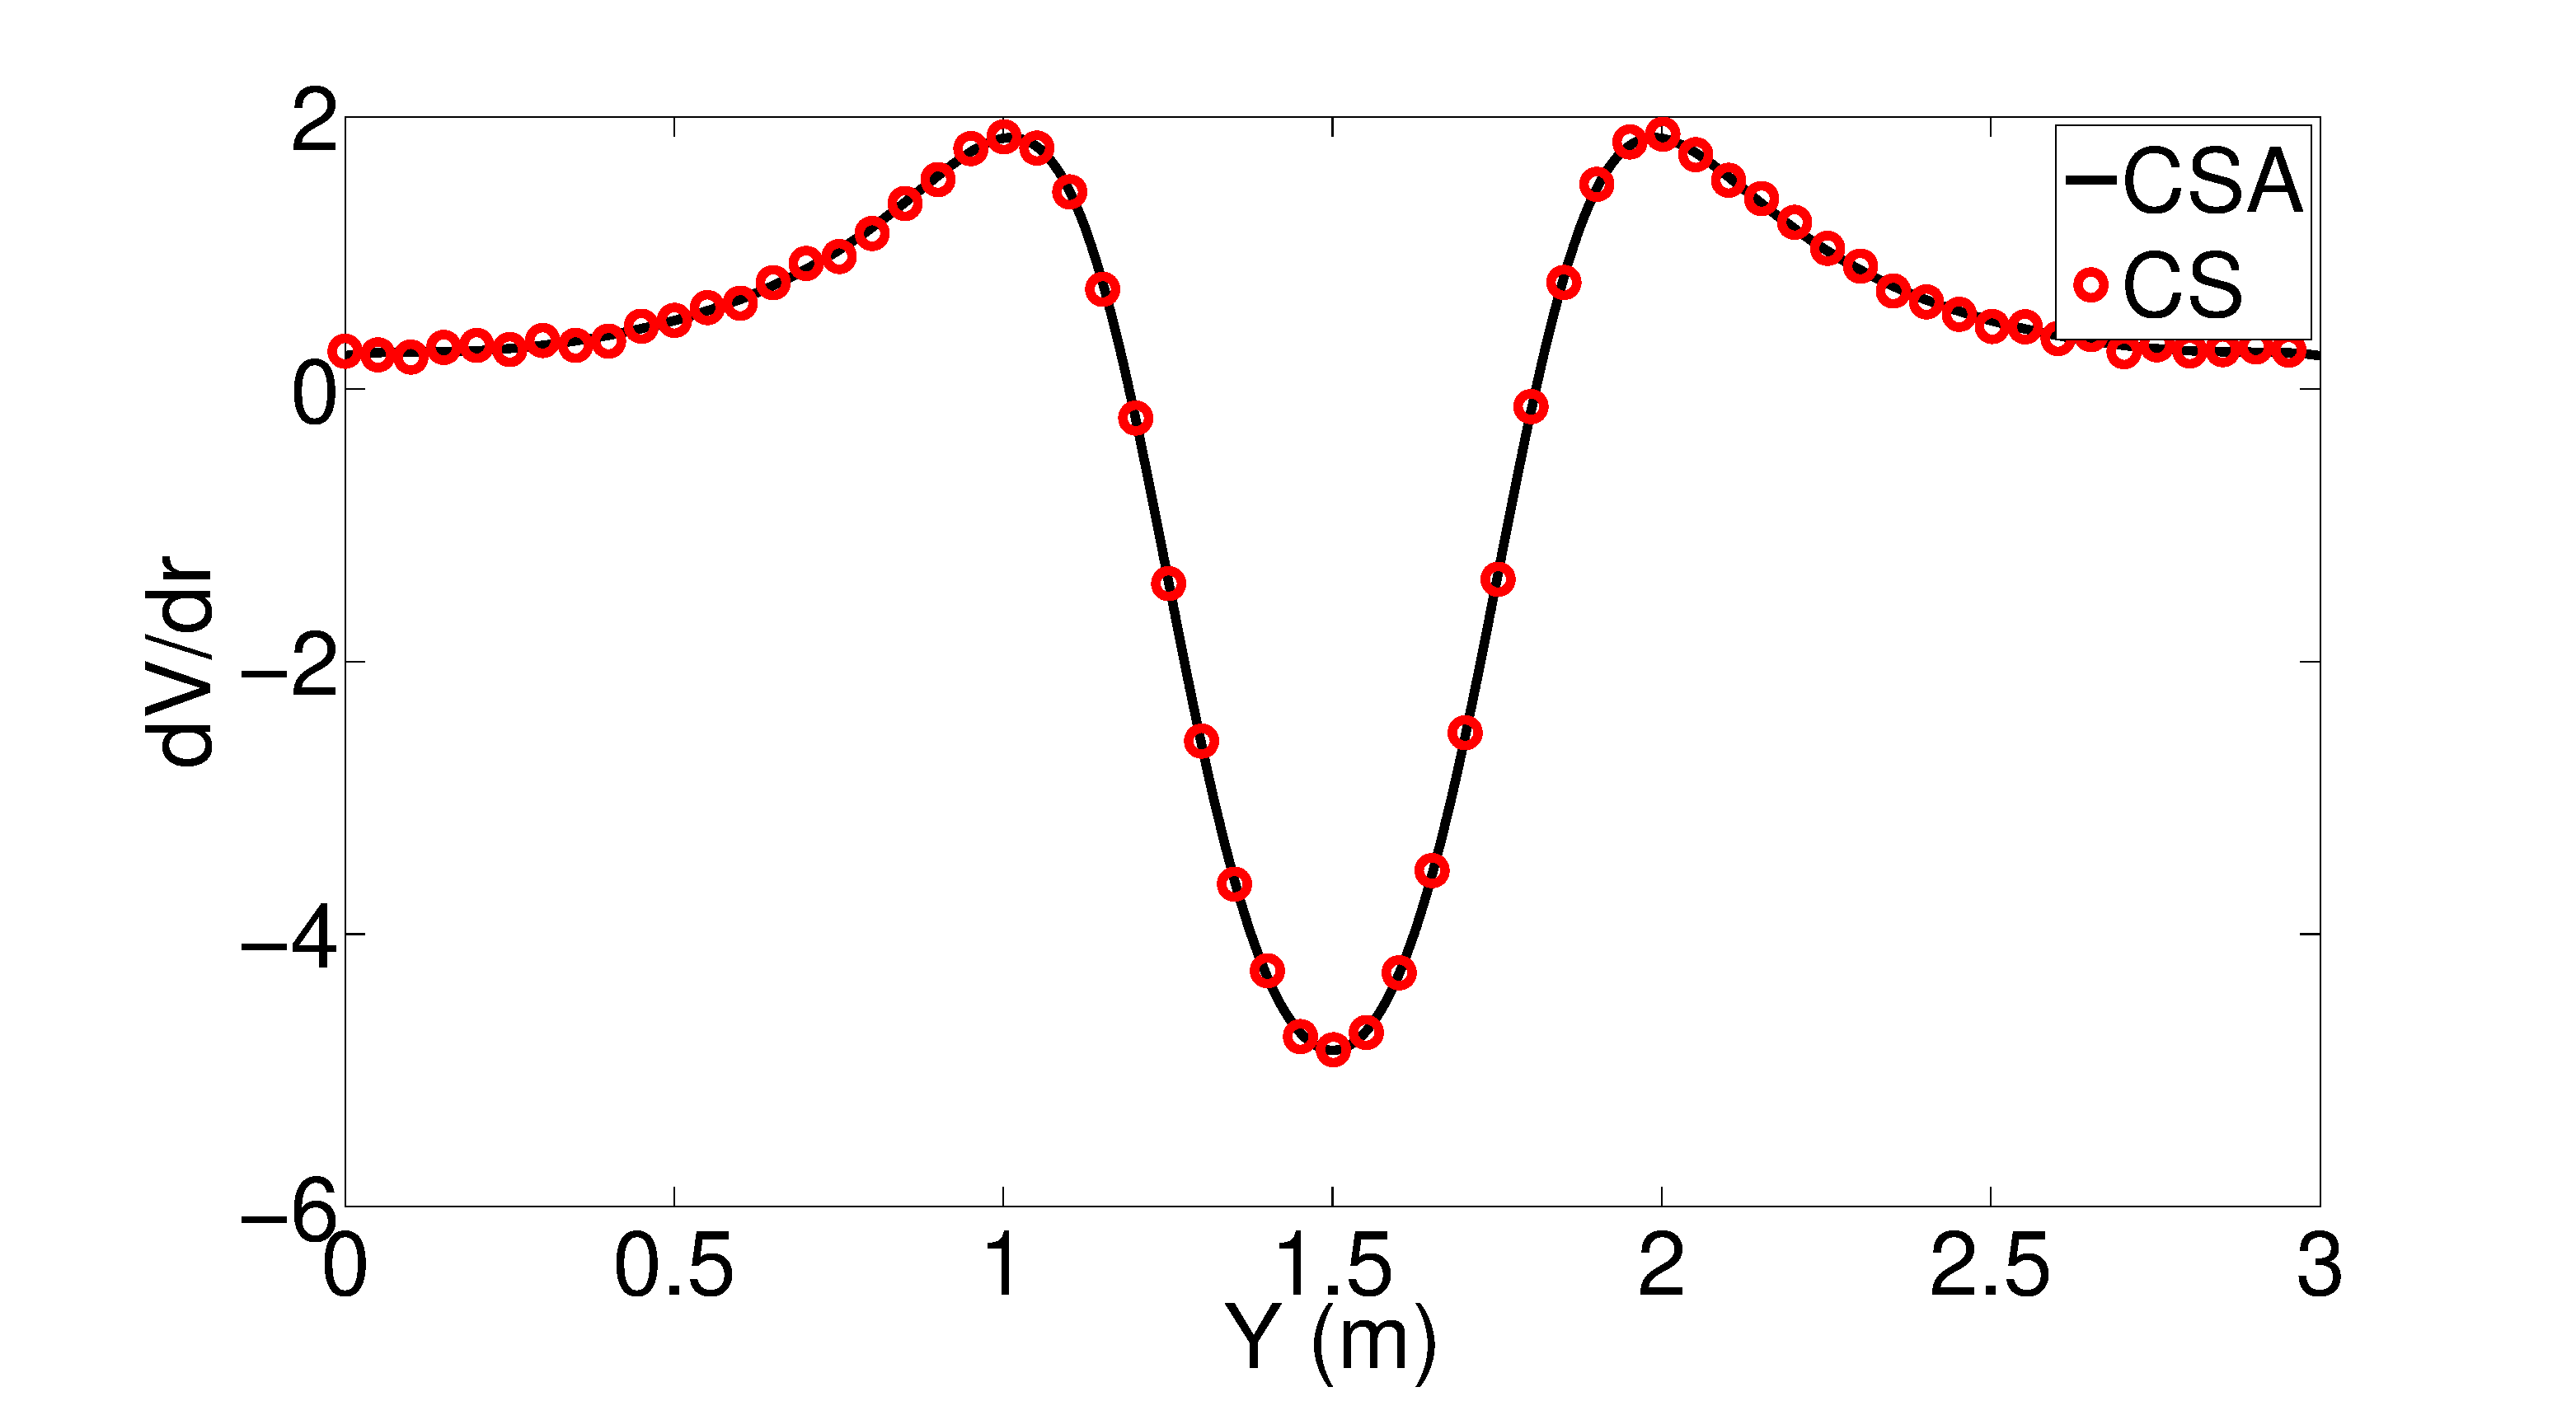
\includegraphics[width=6.5cm]{Chapter_4/figure/flow_over_cylinder/validation_dVdR_X200_RE100.eps}
    }
    \\
	\subfigure[Pressure sensitivity on $y = 1.50$]
    {
    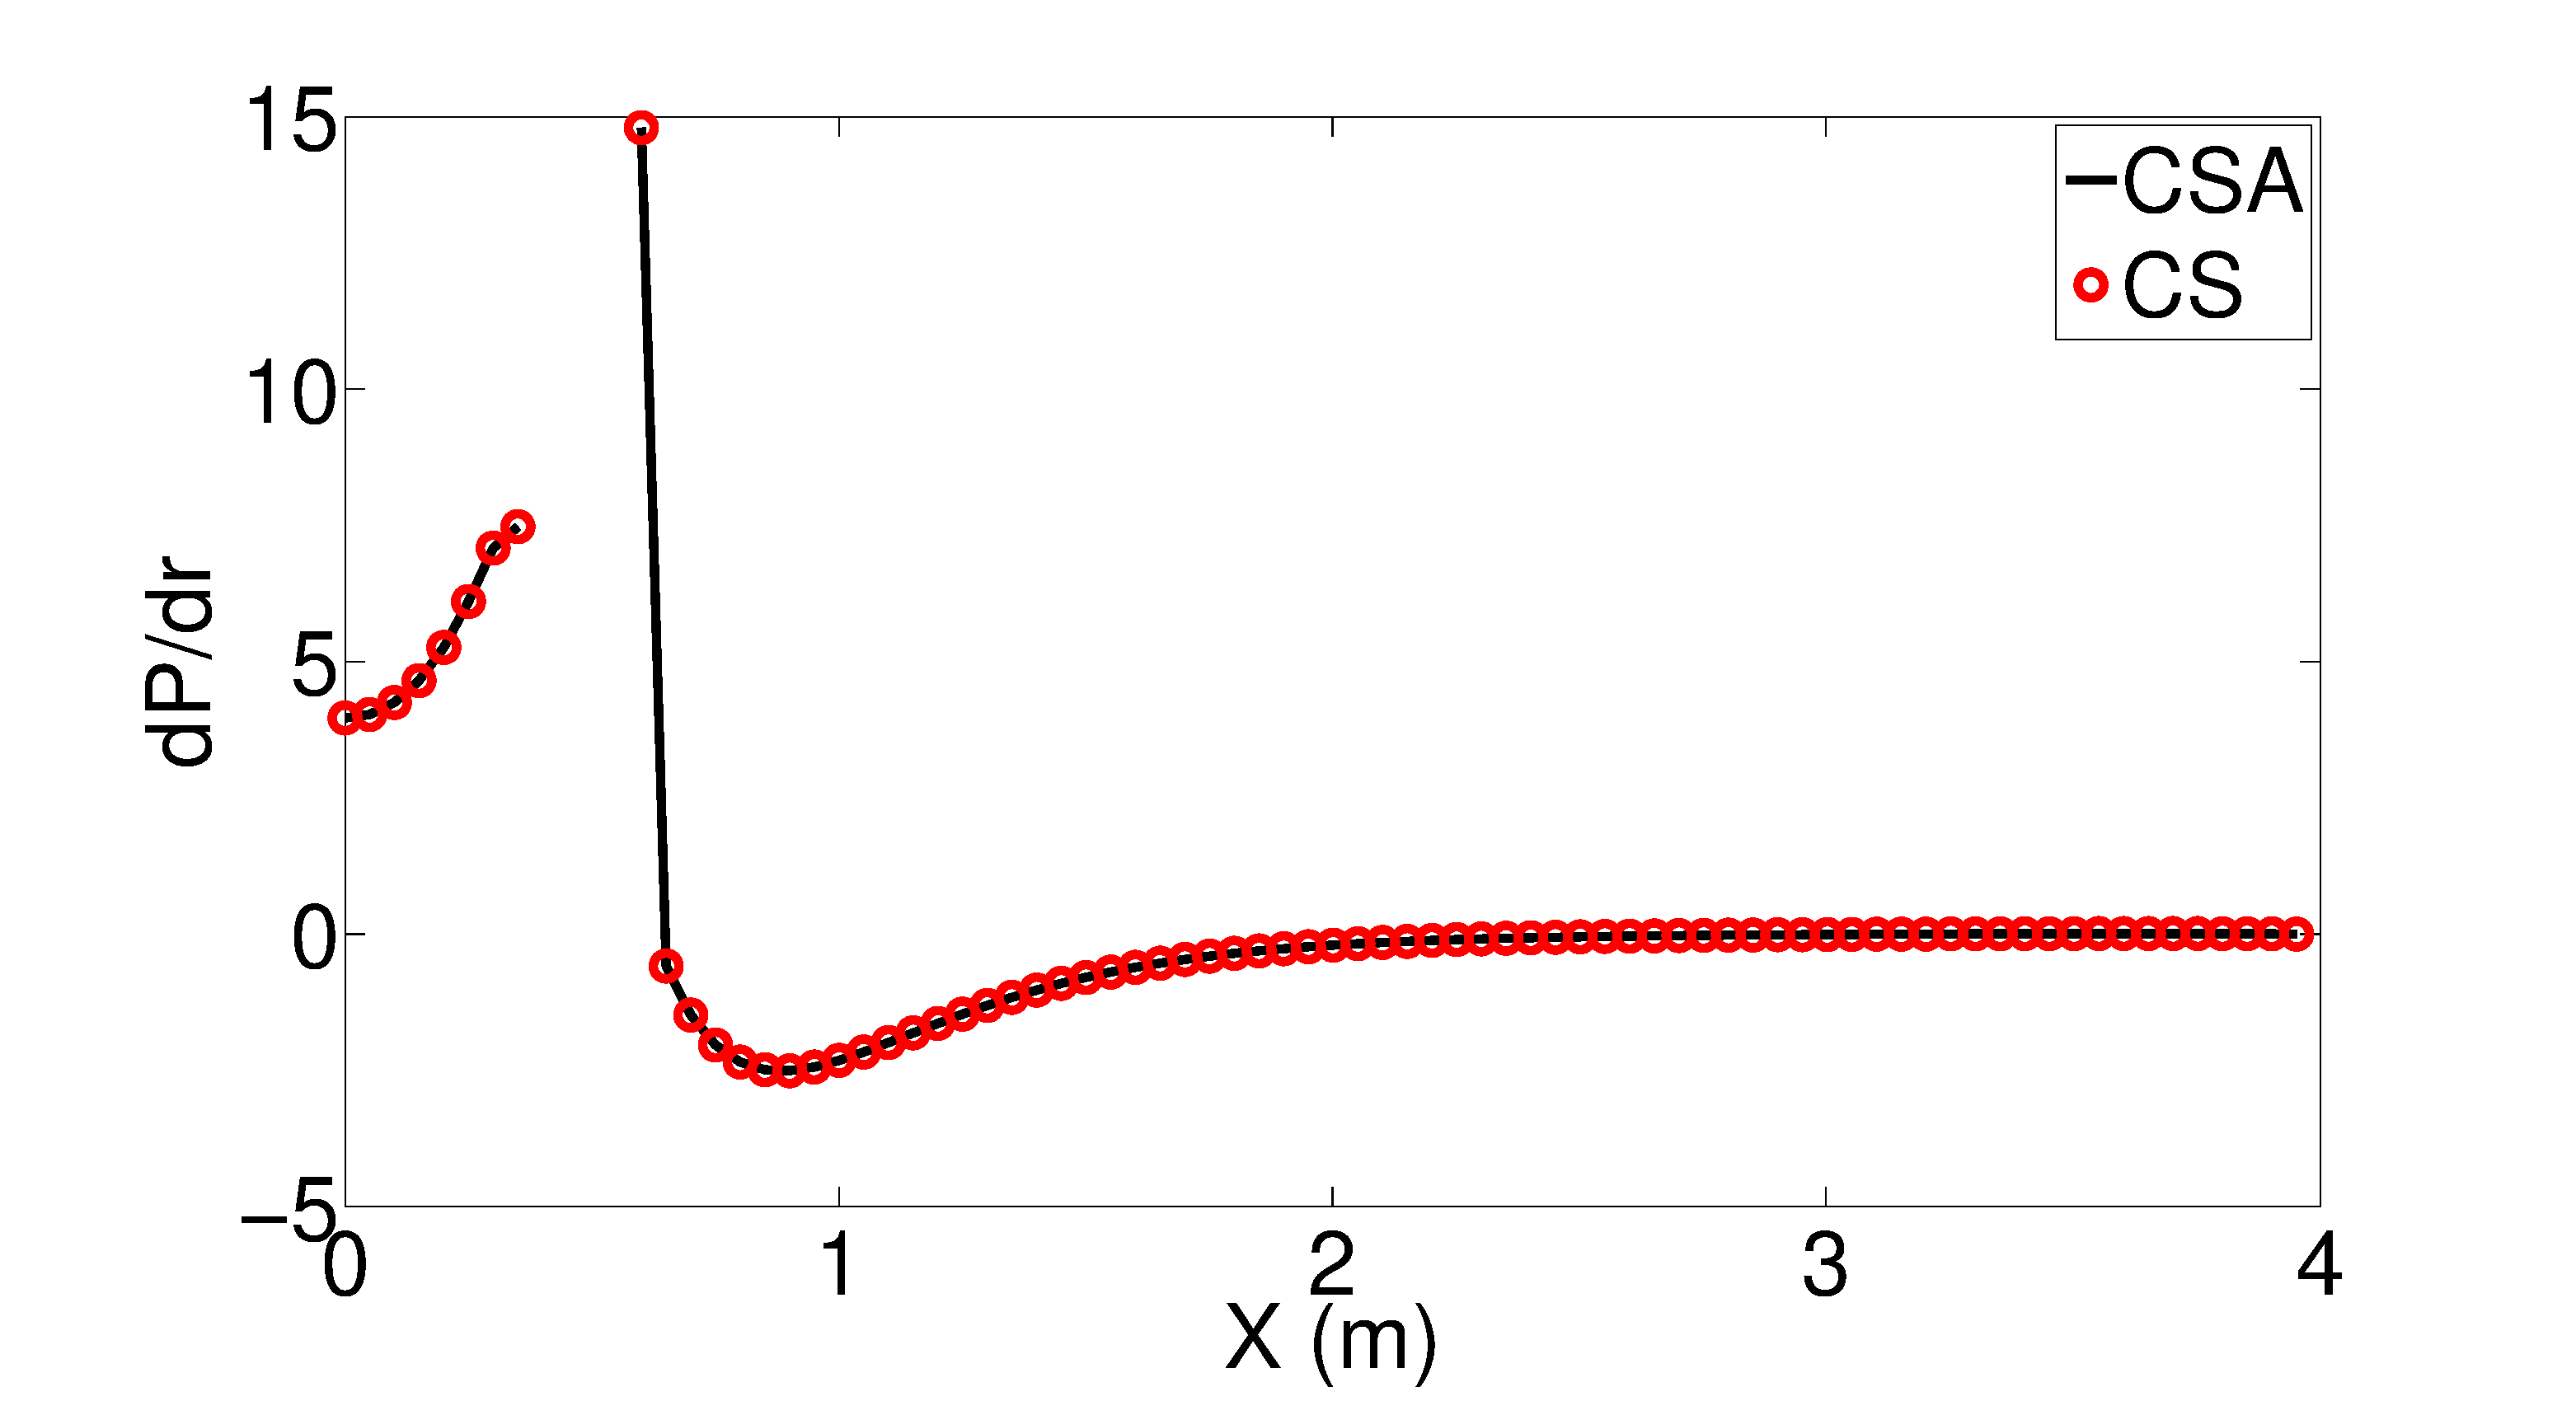
\includegraphics[width=6.5cm]{Chapter_4/figure/flow_over_cylinder/validation_dPdR_Y150_RE100.eps}
    }
    \quad
    \subfigure[Pressure sensitivity on $x = 2.00$]
    {
    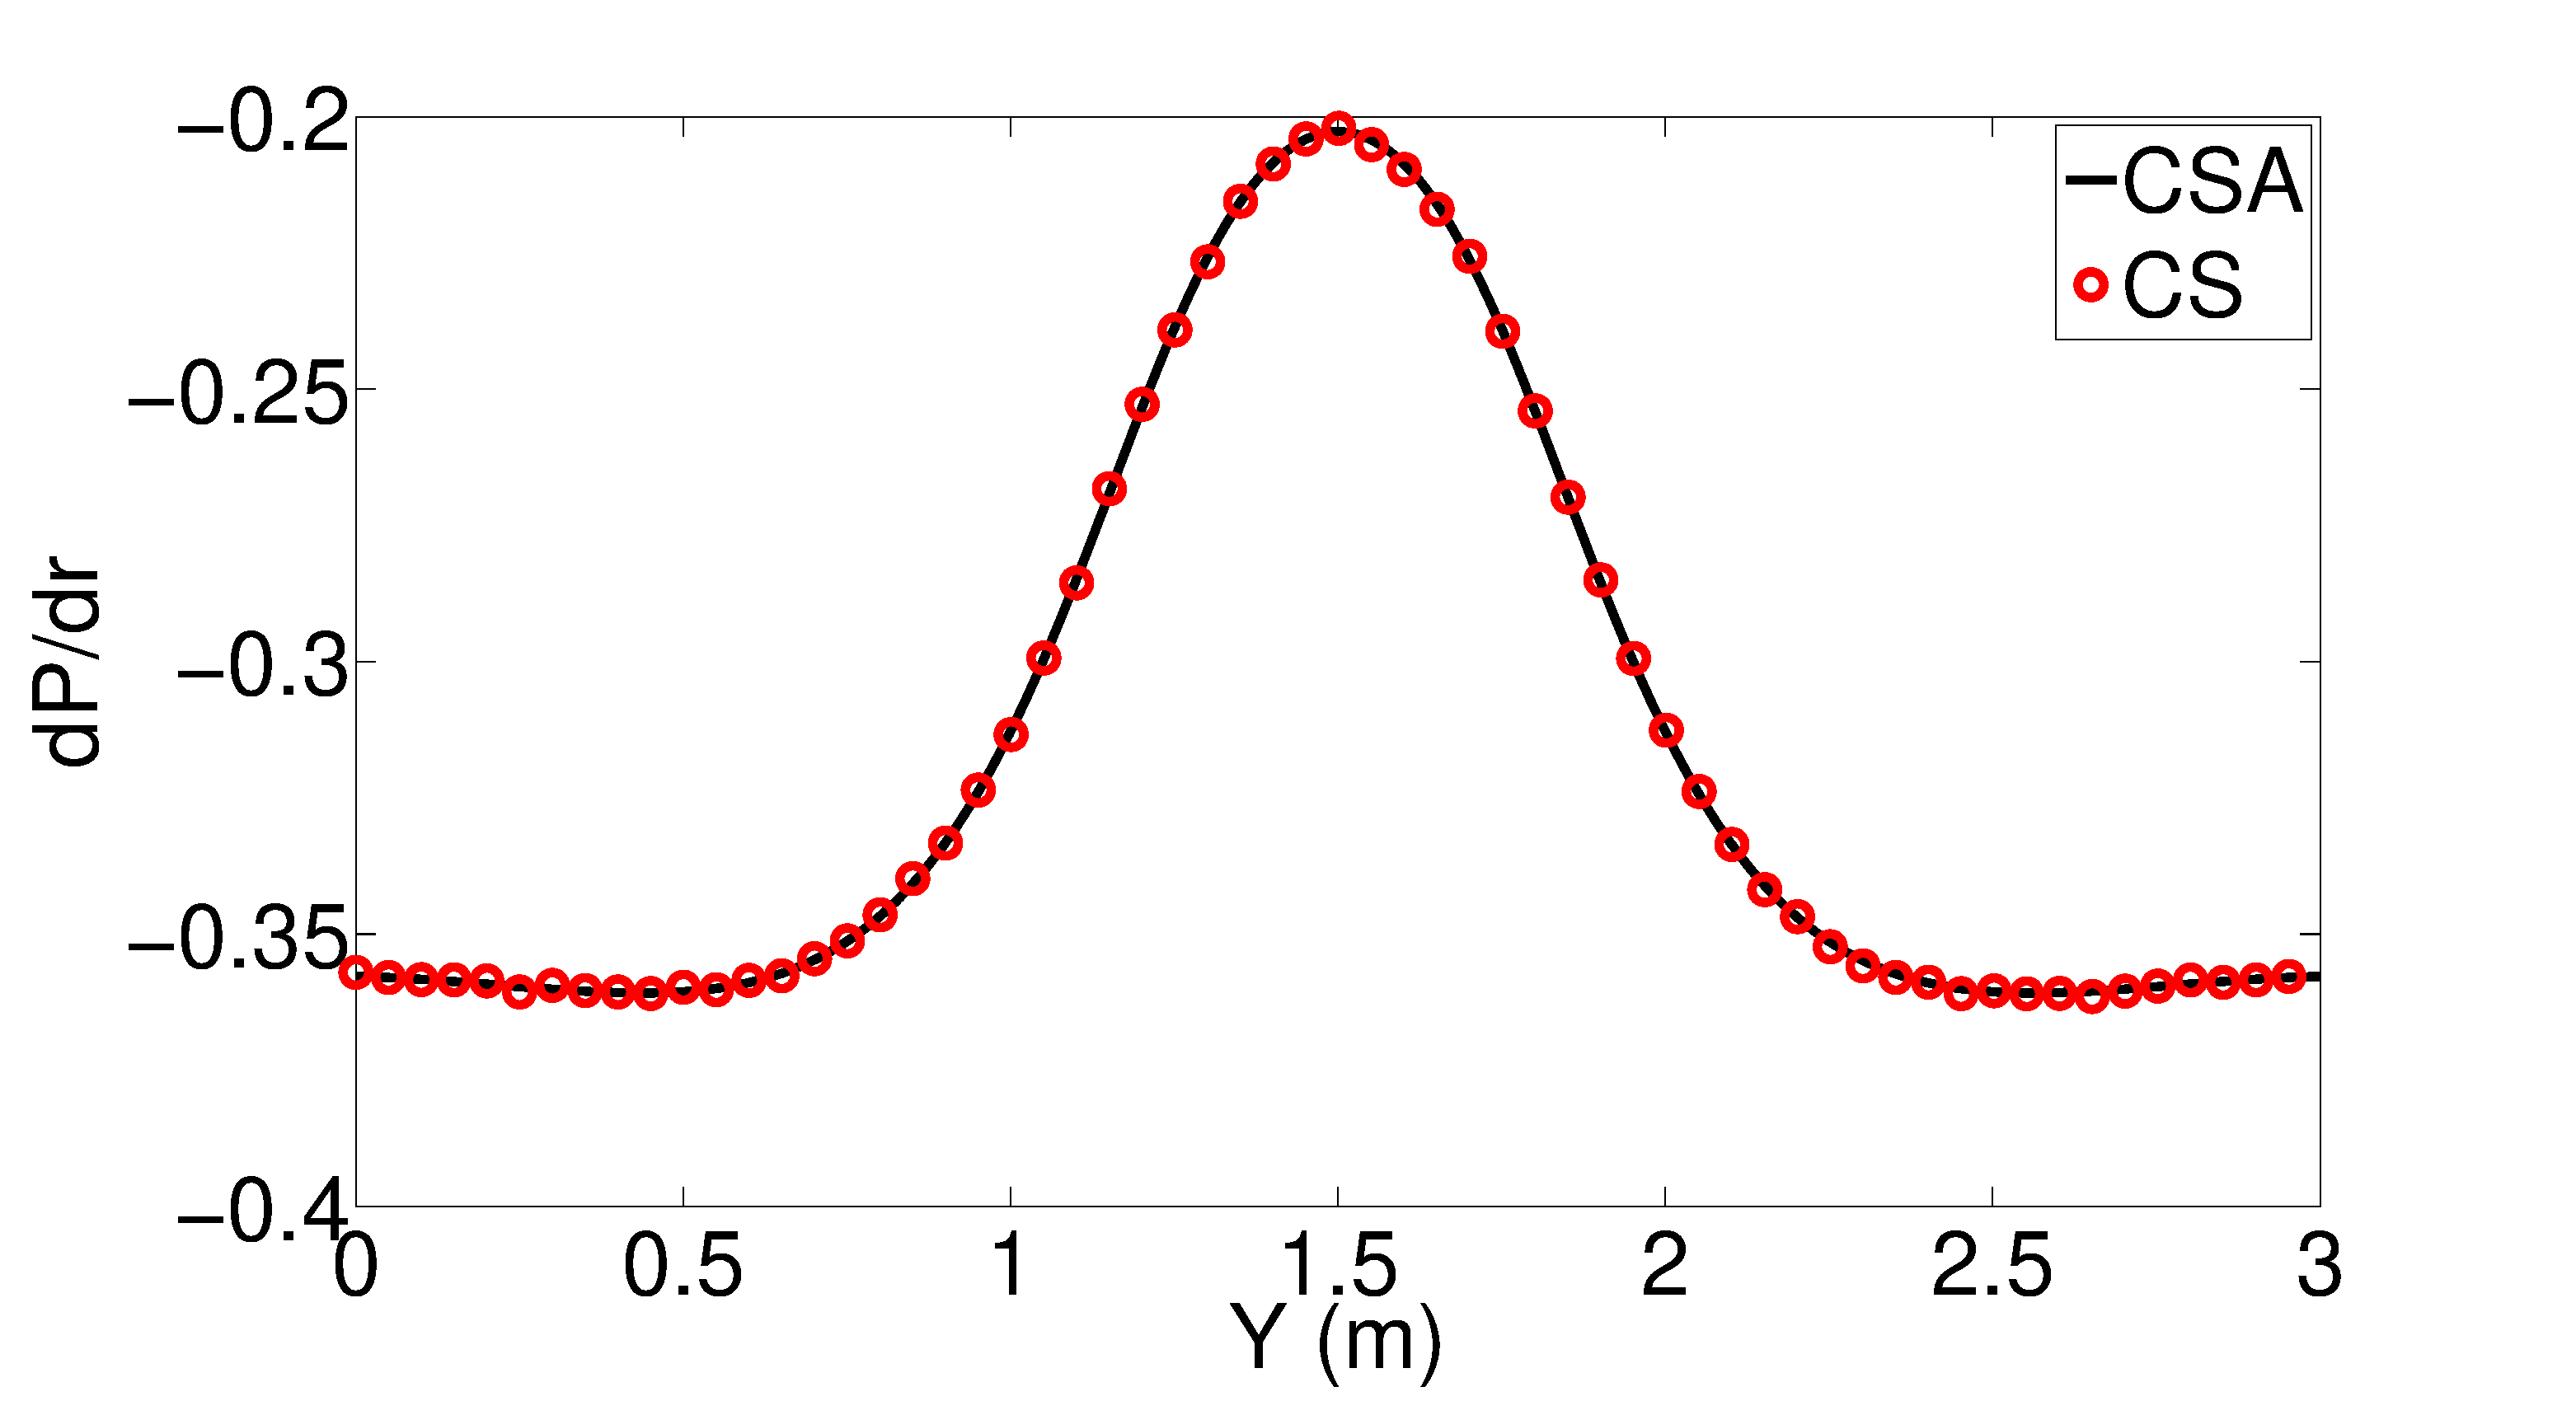
\includegraphics[width=6.5cm]{Chapter_4/figure/flow_over_cylinder/validation_dPdR_X200_RE100.eps}
    }
    \caption{Verification of the flow variable sensitivities with respect to change in the cylinder radius for different location in the domain.}
    \label{fig:C4_flowOverCylinderSensitivityValidation}
\end{figure}
%
The rate of convergence of the sensitivity results are investigated in Figure \ref{fig:C4_flowOverCylinderSArateOfConvergence}. The slope of the fitted line (dashed line) for $u$-velocity, $v$-velocity, and pressure sensitivity are reported as $-2.2$, $-1.94$, and $-2.31$, respectively. The $v$-velocity has lower convergence rate since the sampling location is near the wall where the spatial approximations are first order.
%
\begin{figure}[H]
    \centering
    \subfigure[U-velocity sensitivity convergence rate (at $(0.0, 1.5)$)]
    {
    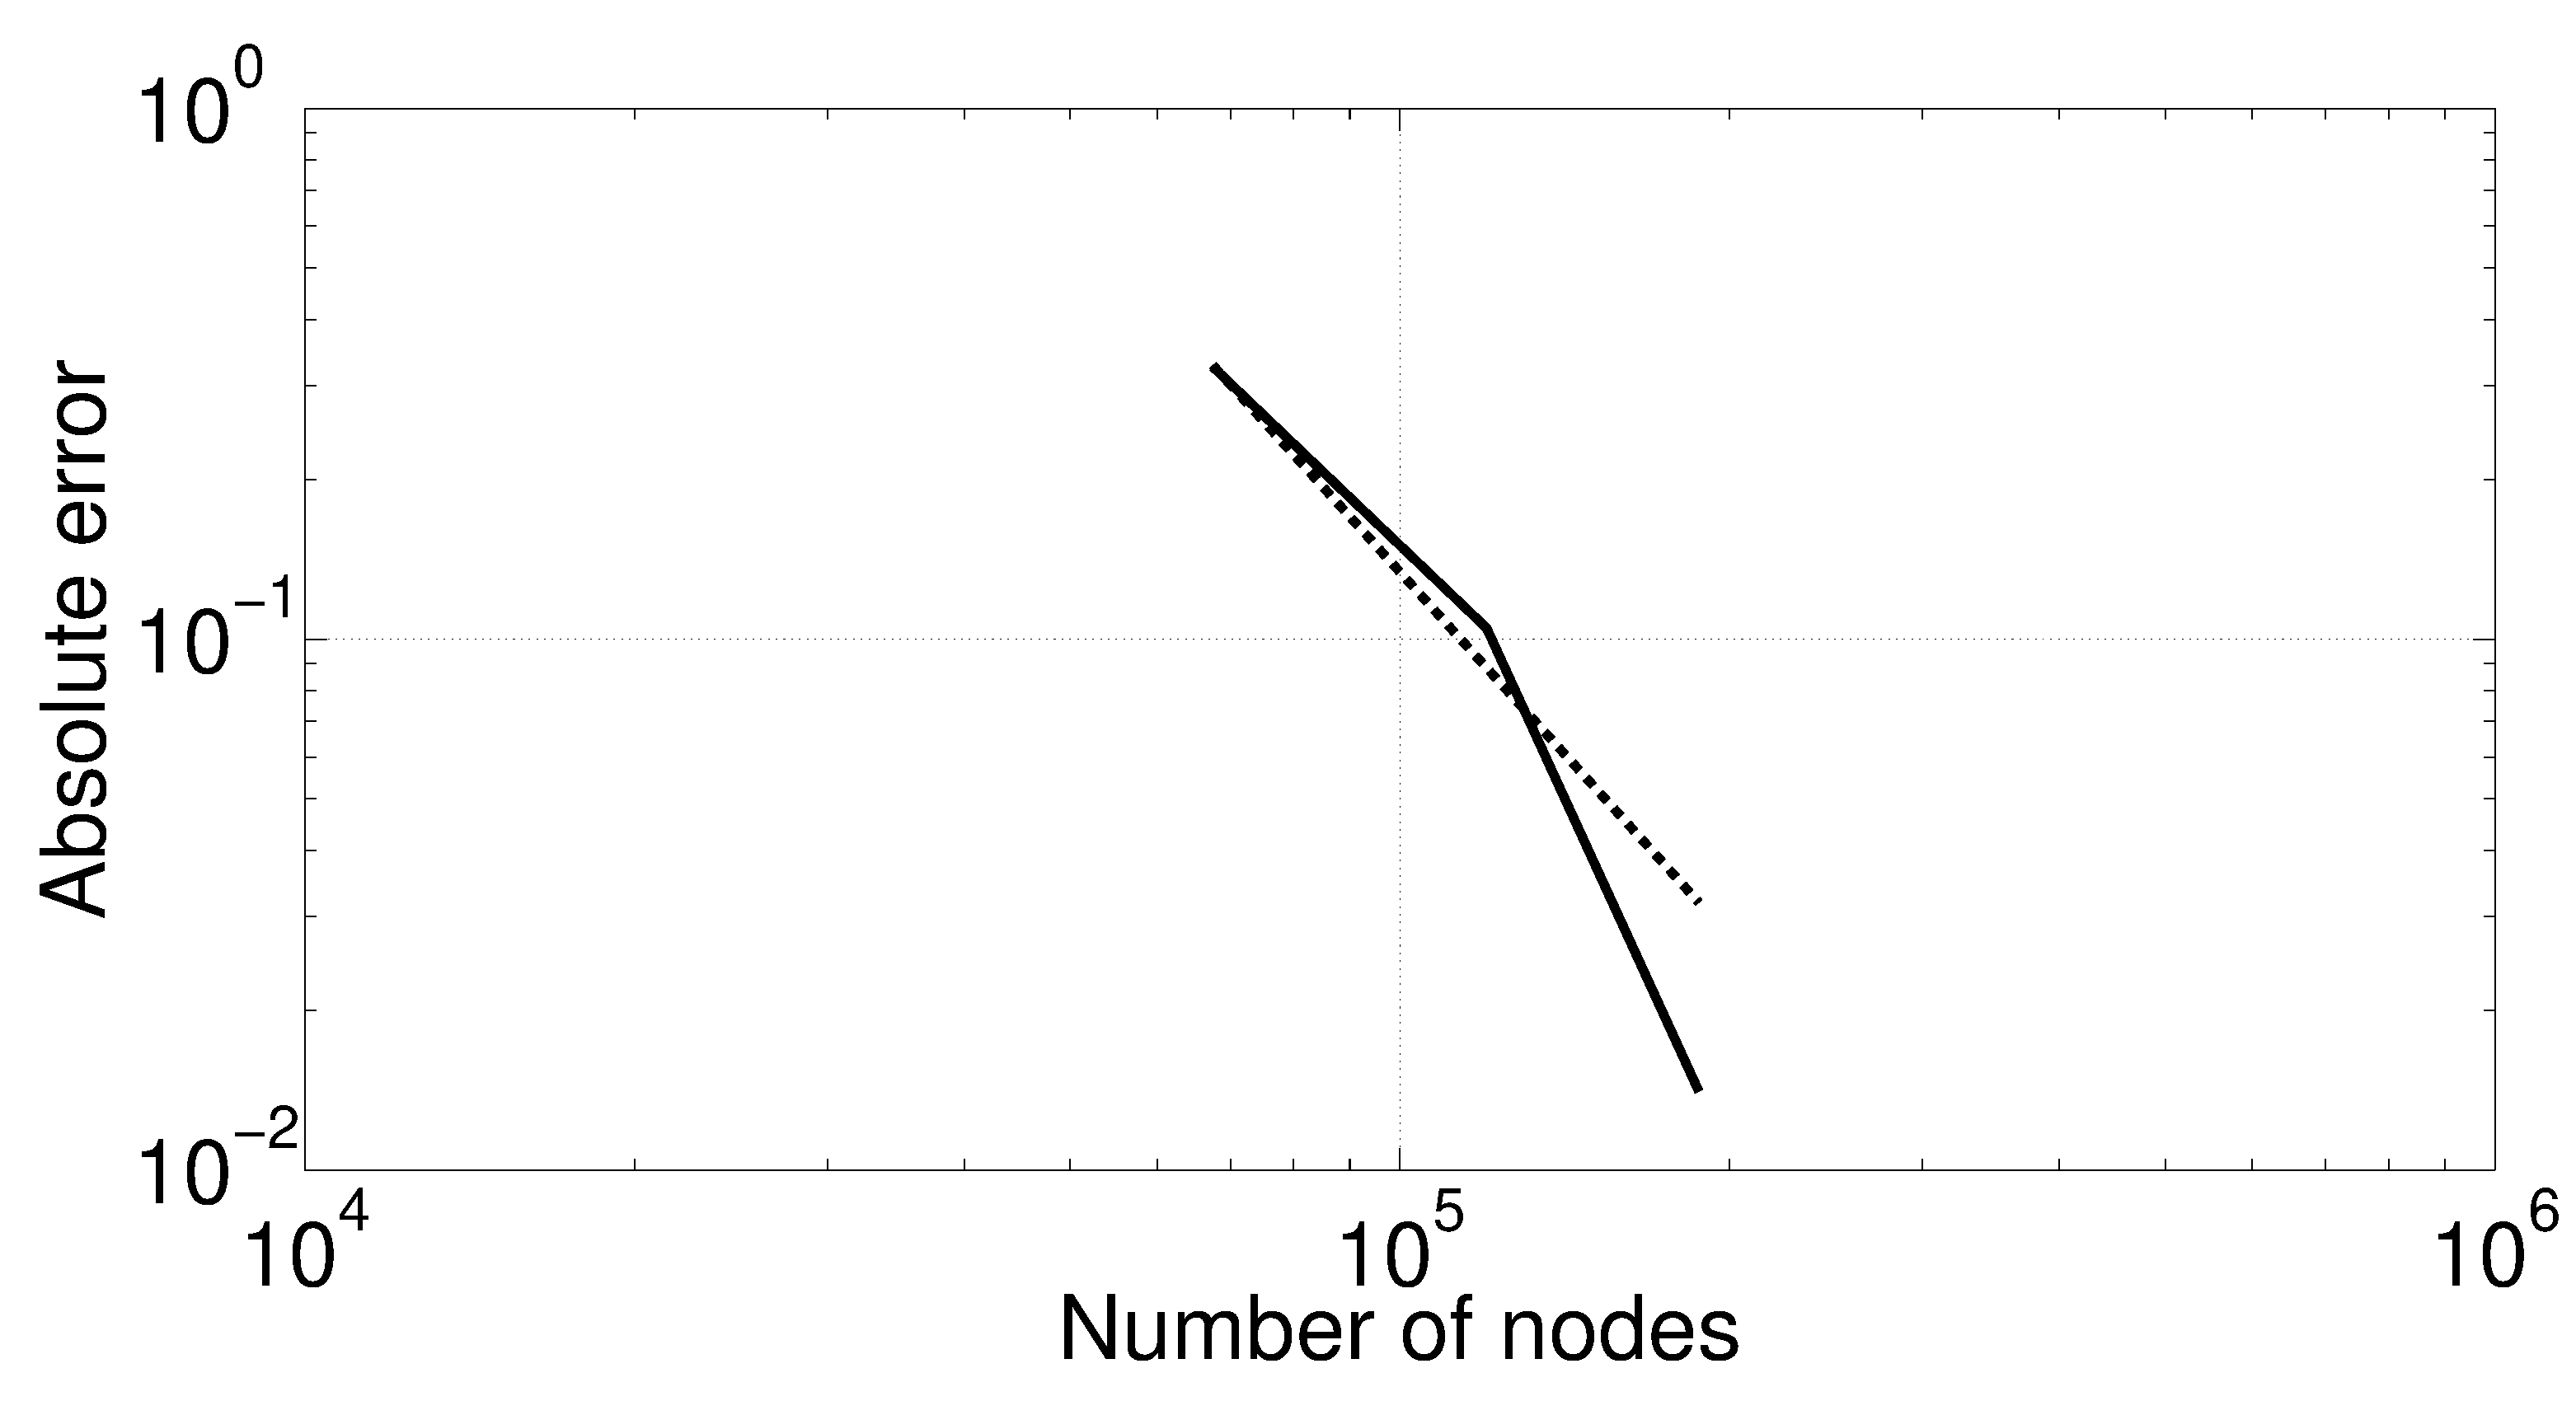
\includegraphics[width=6.5cm]{Chapter_4/figure/flow_over_cylinder/convergenceRate_dUdR_RE100.eps}
    }
    \quad
    \subfigure[V-velocity sensitivity convergence rate (at $(0.5, 0.75)$)]
    {
    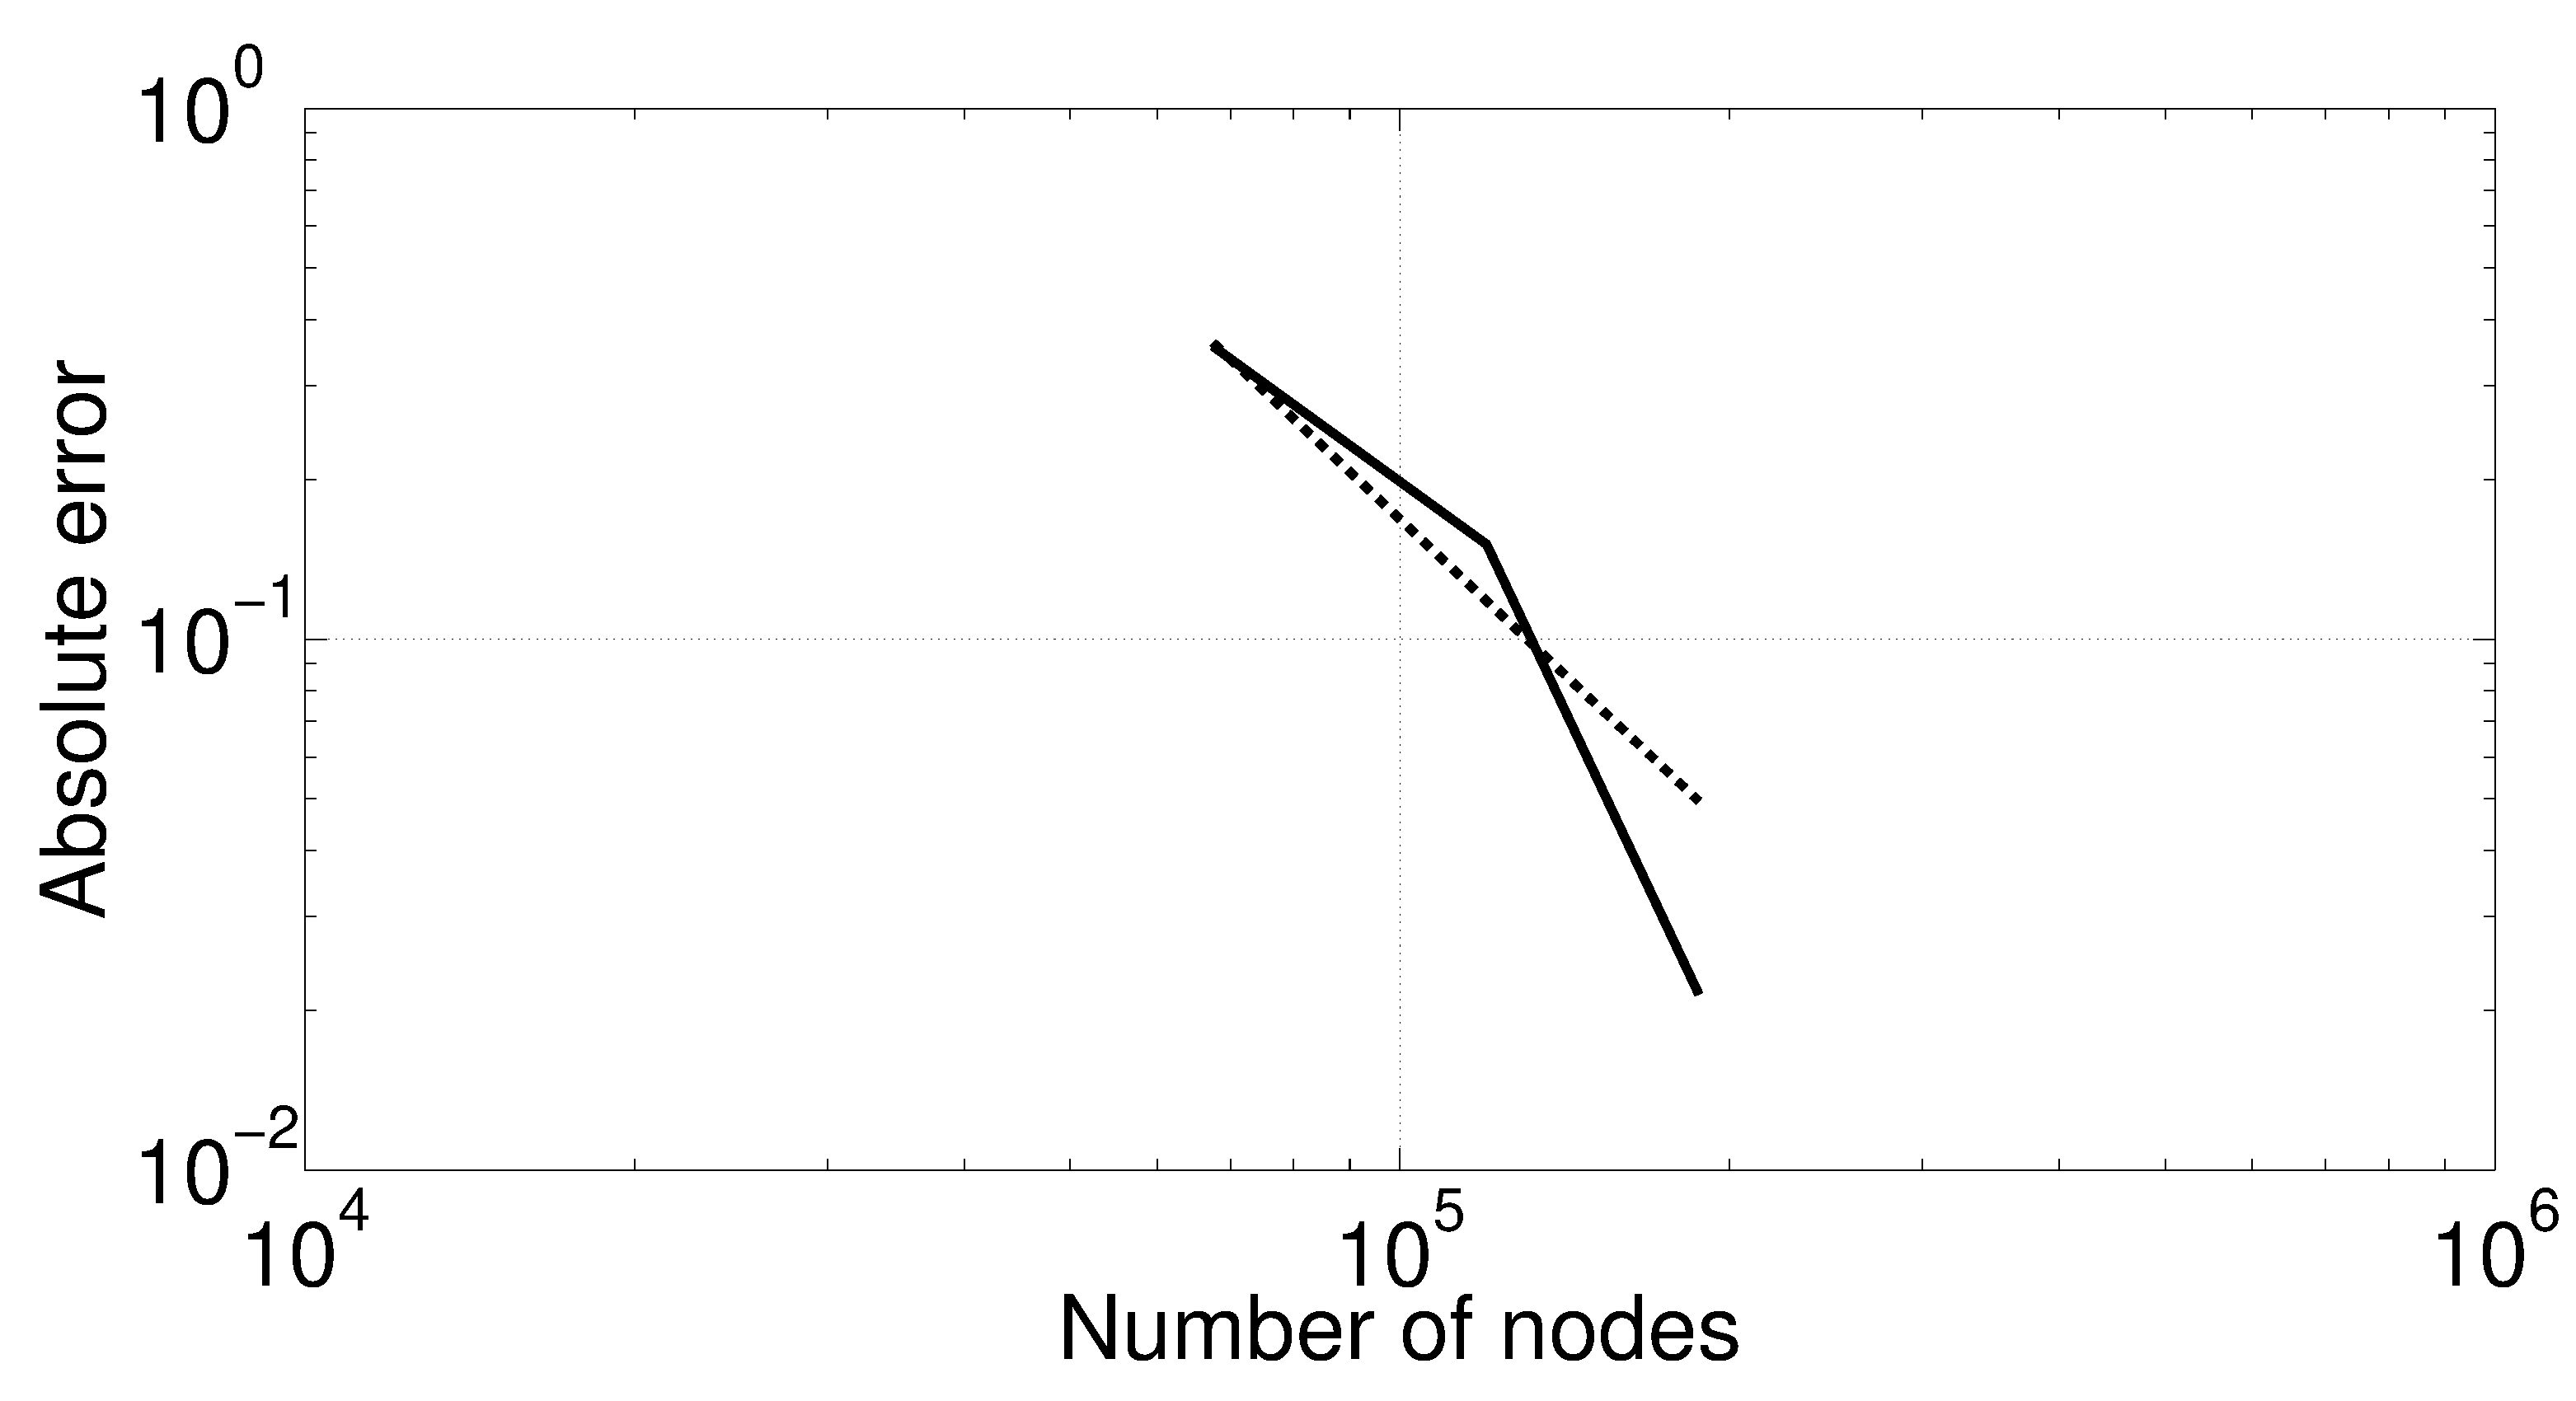
\includegraphics[width=6.5cm]{Chapter_4/figure/flow_over_cylinder/convergenceRate_dVdR_RE100.eps}
    }
    \\
    \subfigure[Pressure sensitivity convergence rate (at $(0.0, 1.0)$)]
    {
    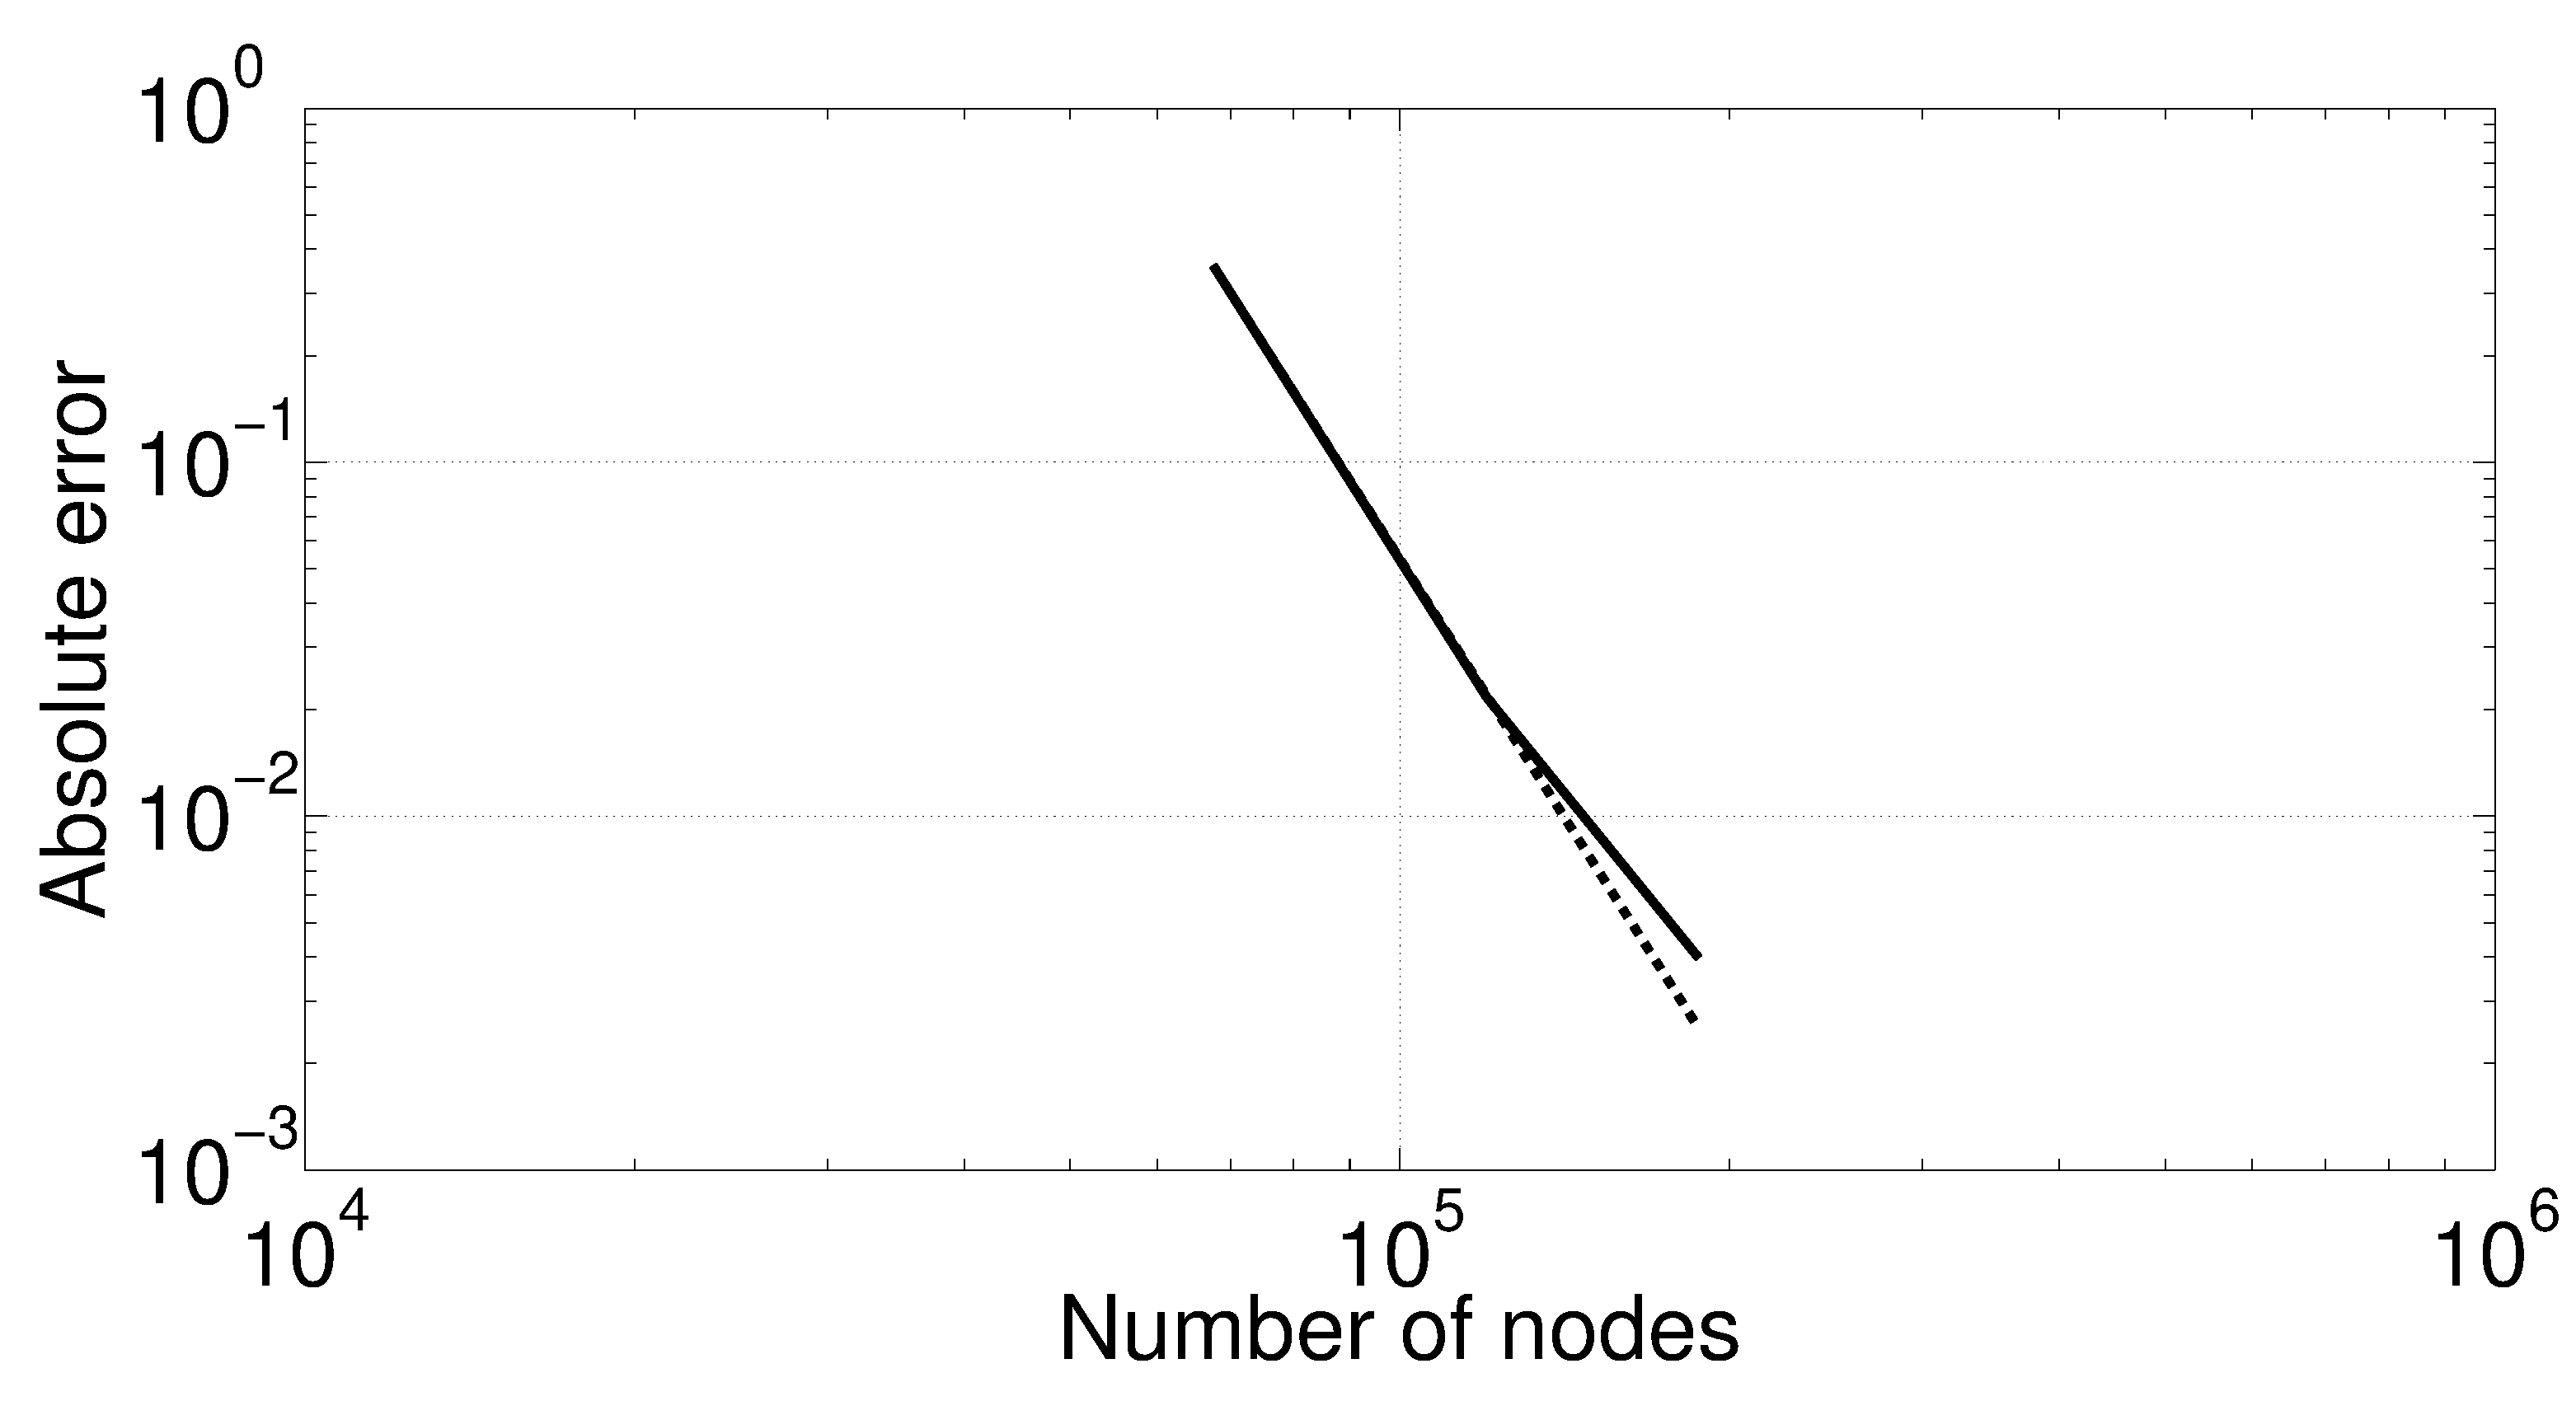
\includegraphics[width=6.5cm]{Chapter_4/figure/flow_over_cylinder/convergenceRate_dPdR_RE100.eps}
    }
    \caption{Convergence rate for the sensitivities (Re = 100).}
    \label{fig:C4_flowOverCylinderSArateOfConvergence}
\end{figure}
%
The sensitivity contours for the velocity and pressure are shown in Figure \ref{fig:C4_flowOverCylinderSensitivityContour}.
%
\begin{figure}[H]
    \centering
    \subfigure[U-velocity sensitivity contour]
    {
    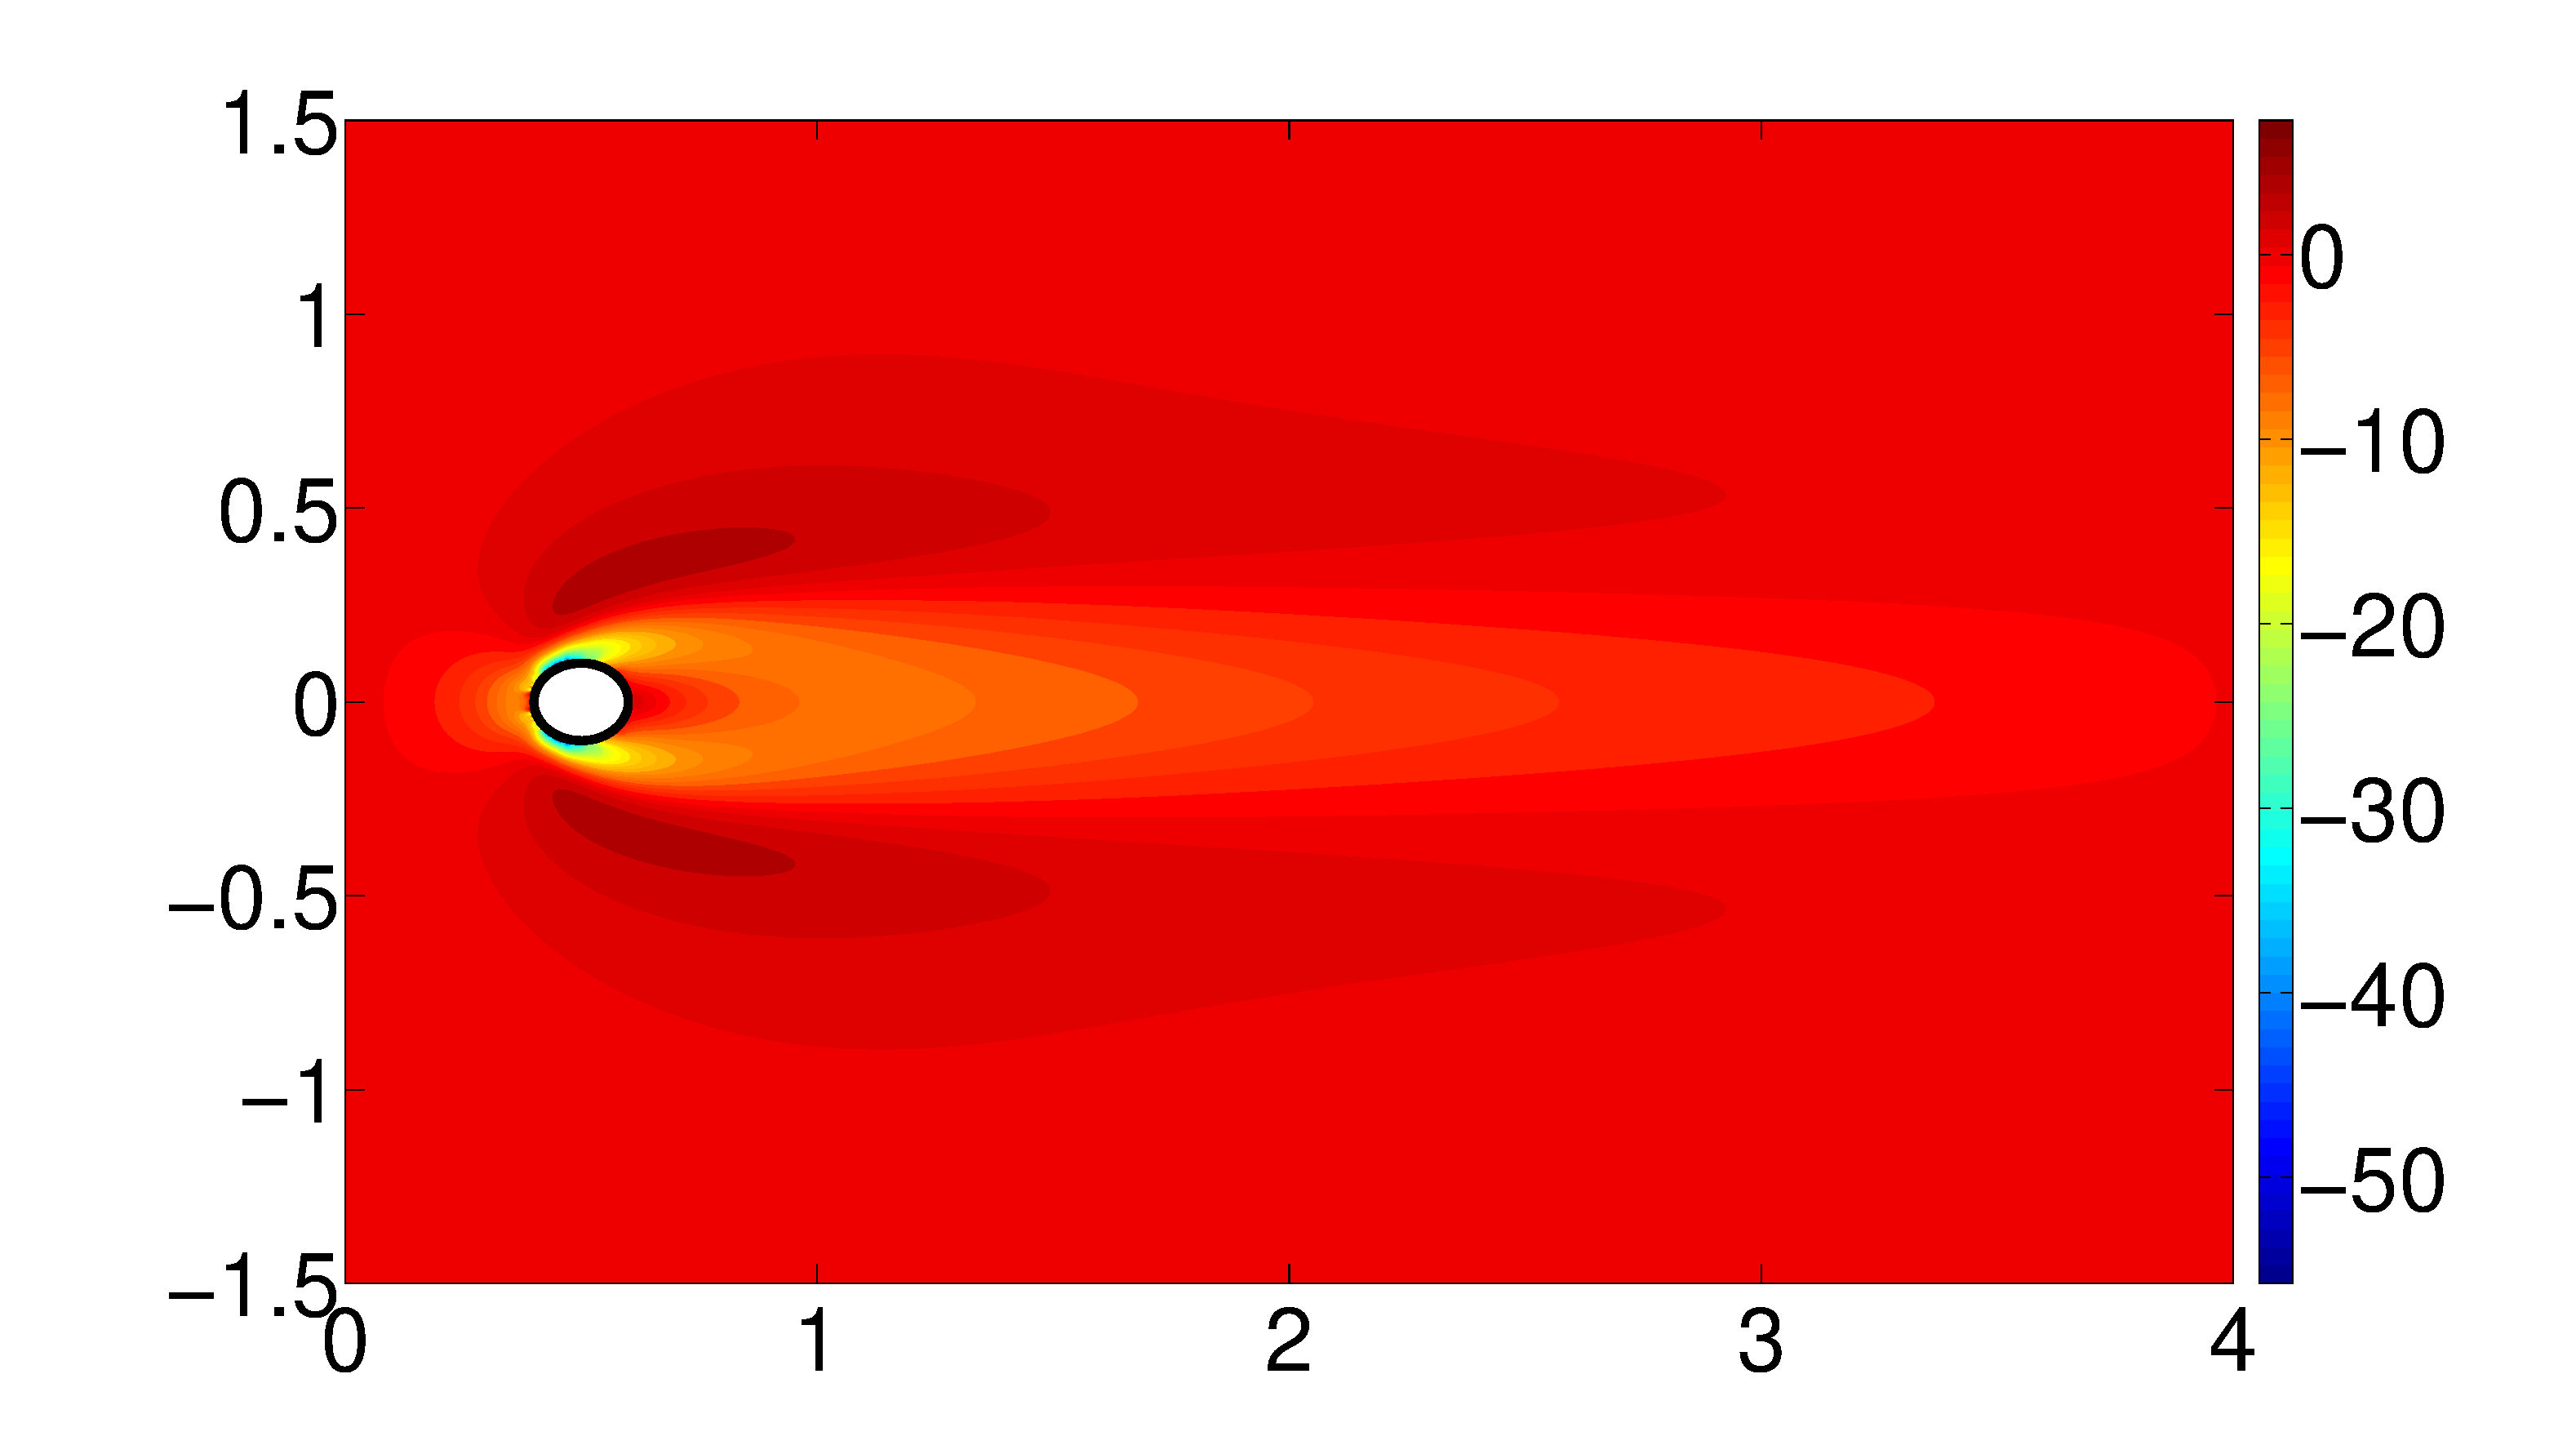
\includegraphics[width=6.5cm]{Chapter_4/figure/flow_over_cylinder/contour_SA_U_RE100.eps}
    }
    \quad
    \subfigure[V-velocity sensitivity contour]
    {
    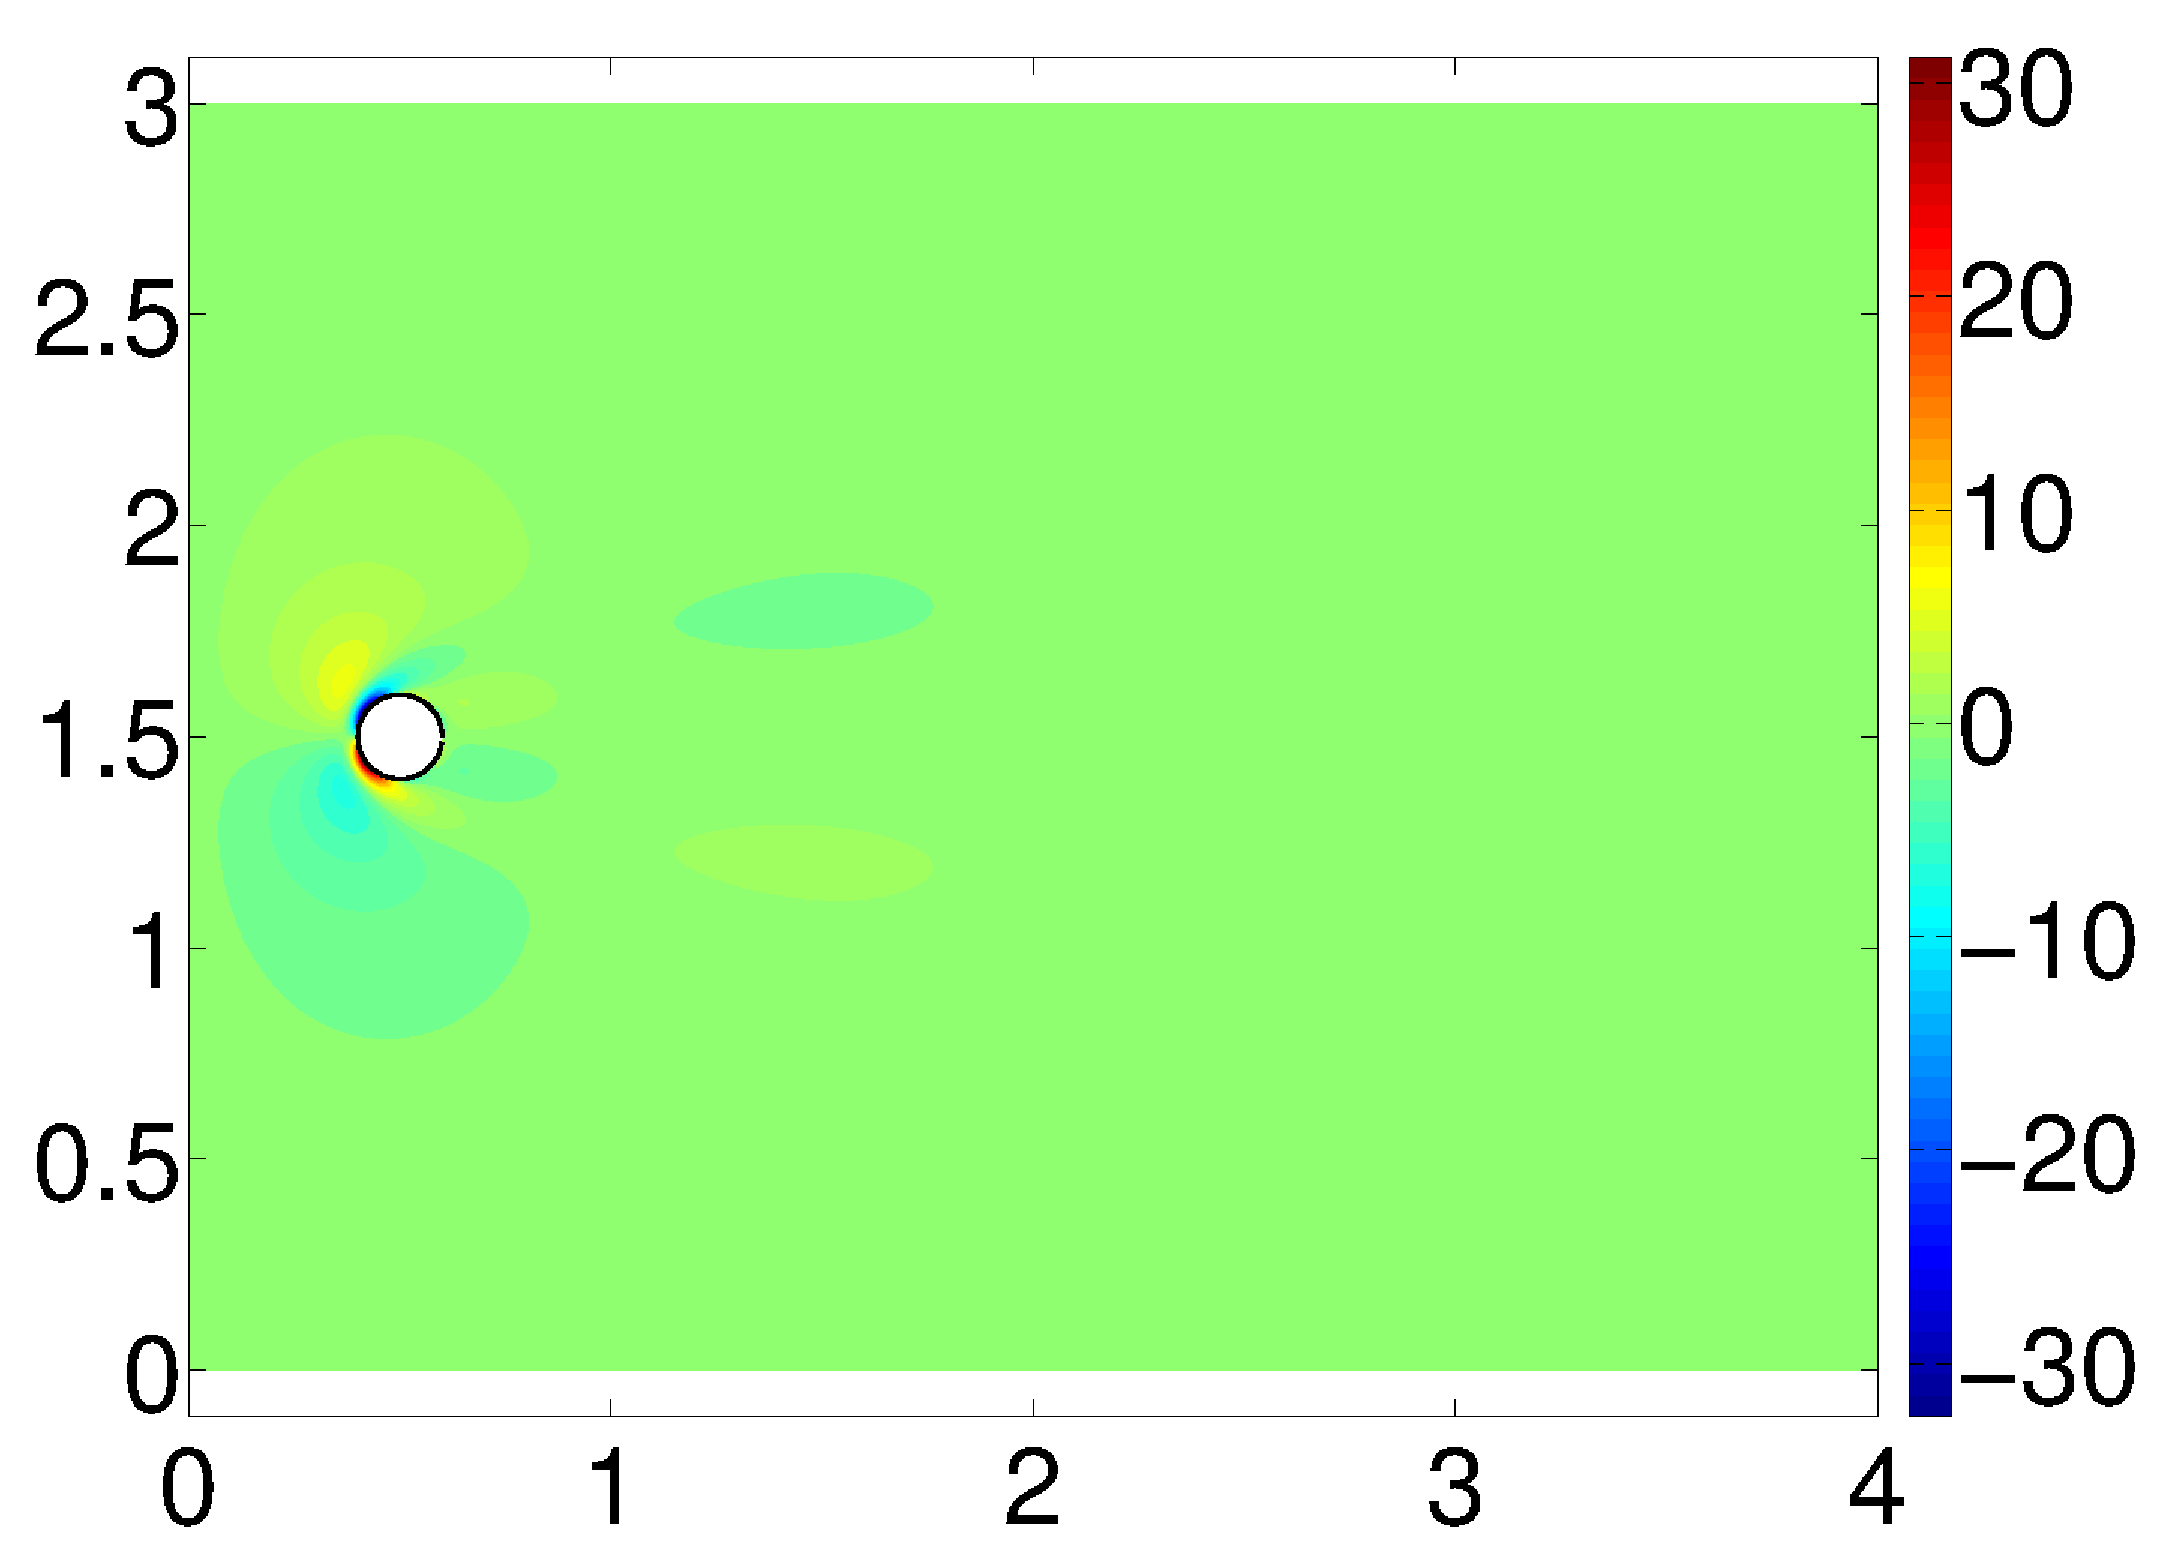
\includegraphics[width=6.5cm]{Chapter_4/figure/flow_over_cylinder/contour_SA_V_RE100.eps}
    }
    \\
    \subfigure[Pressure sensitivity contour]
    {
    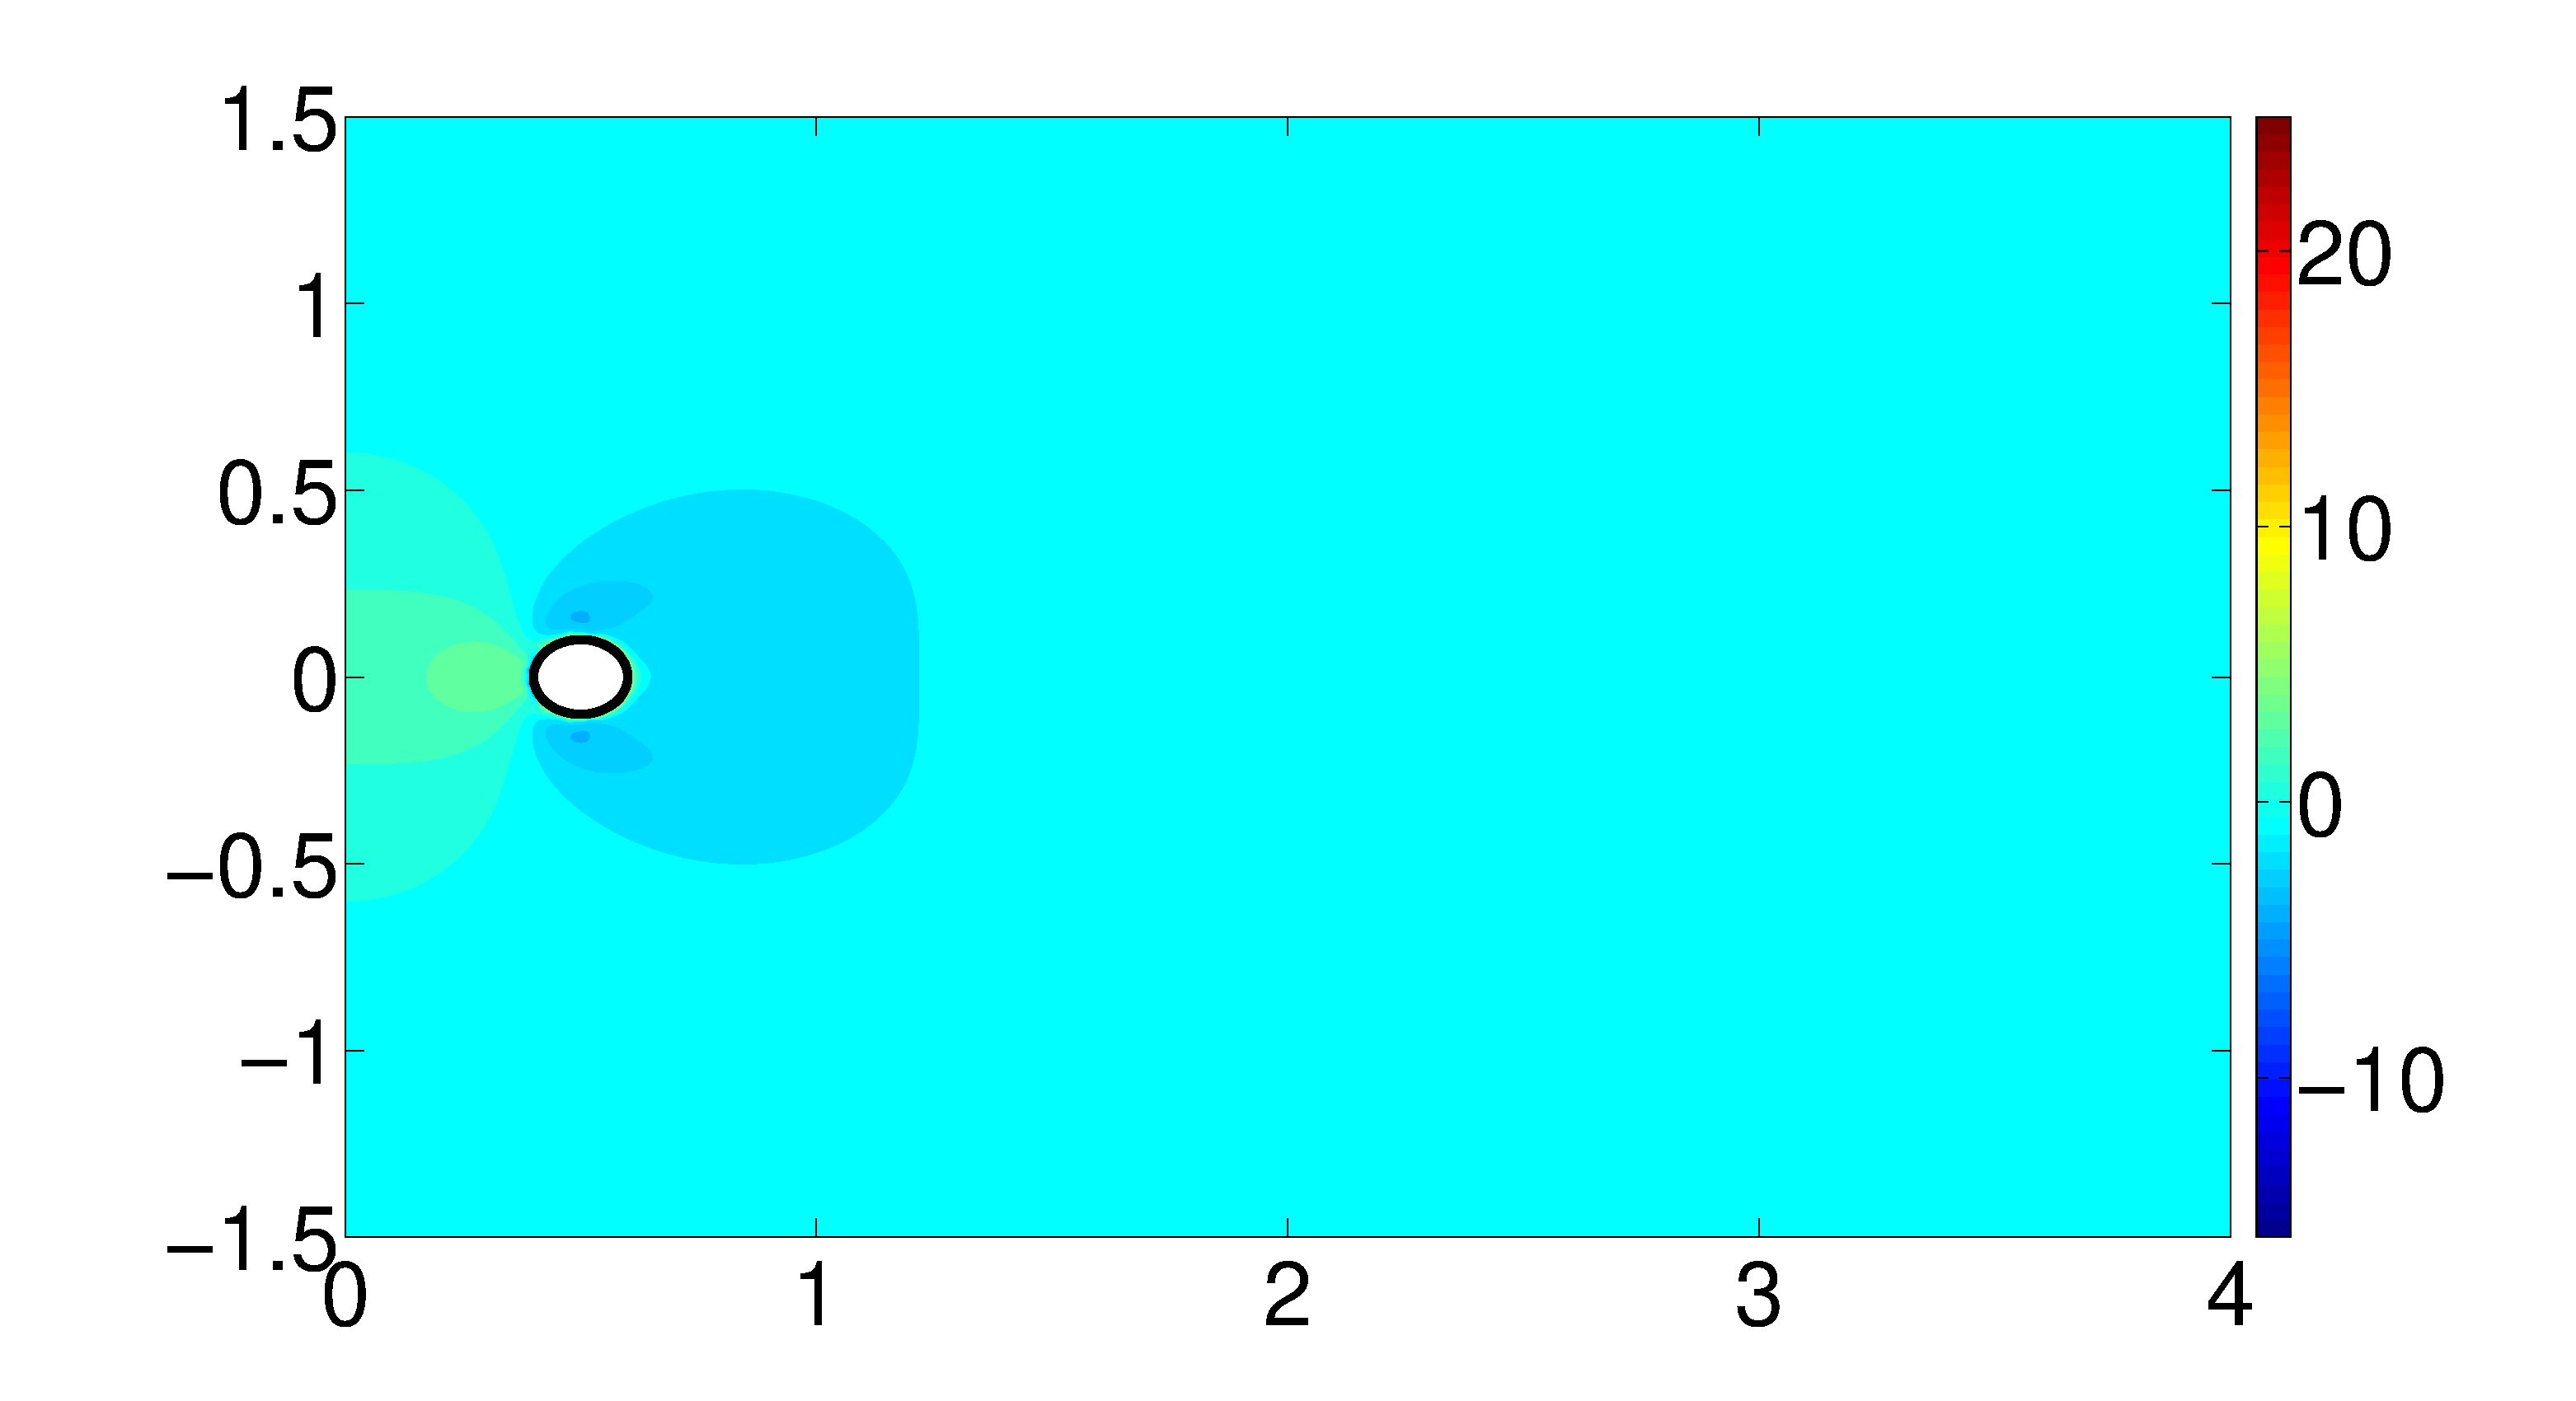
\includegraphics[width=6.5cm]{Chapter_4/figure/flow_over_cylinder/contour_SA_P_RE100.eps}
    }
    \caption{Sensitivity contours for Re = 100.}
    \label{fig:C4_flowOverCylinderSensitivityContour}
\end{figure}
%
In most aerodynamic/aeroelastic designs, the sensitivity analysis is conducted for calculating the sensitivity of the pressure field on the surface of the solid boundaries. This sensitivity value is later used for calculating the sensitivity of aerodynamic forces acting on the solid boundaries by integrating the sensitivity of the pressure field. For this purpose, the sensitivity of the pressure field is plotted on solid boundaries and verified with the complex step method in Figure \ref{fig:C4_flowOverCylidner_pressureSensitivityOnSurface}. It should be noted that Savitzky-Golay filtering is used to smooth the sensitivity results over the solid boundary. As shown in Figure \ref{fig:C4_flowOverCylidner_pressureSensitivityOnSurface}, the two results agree very well with each other.
%
\begin{figure}[H]
    \centering
    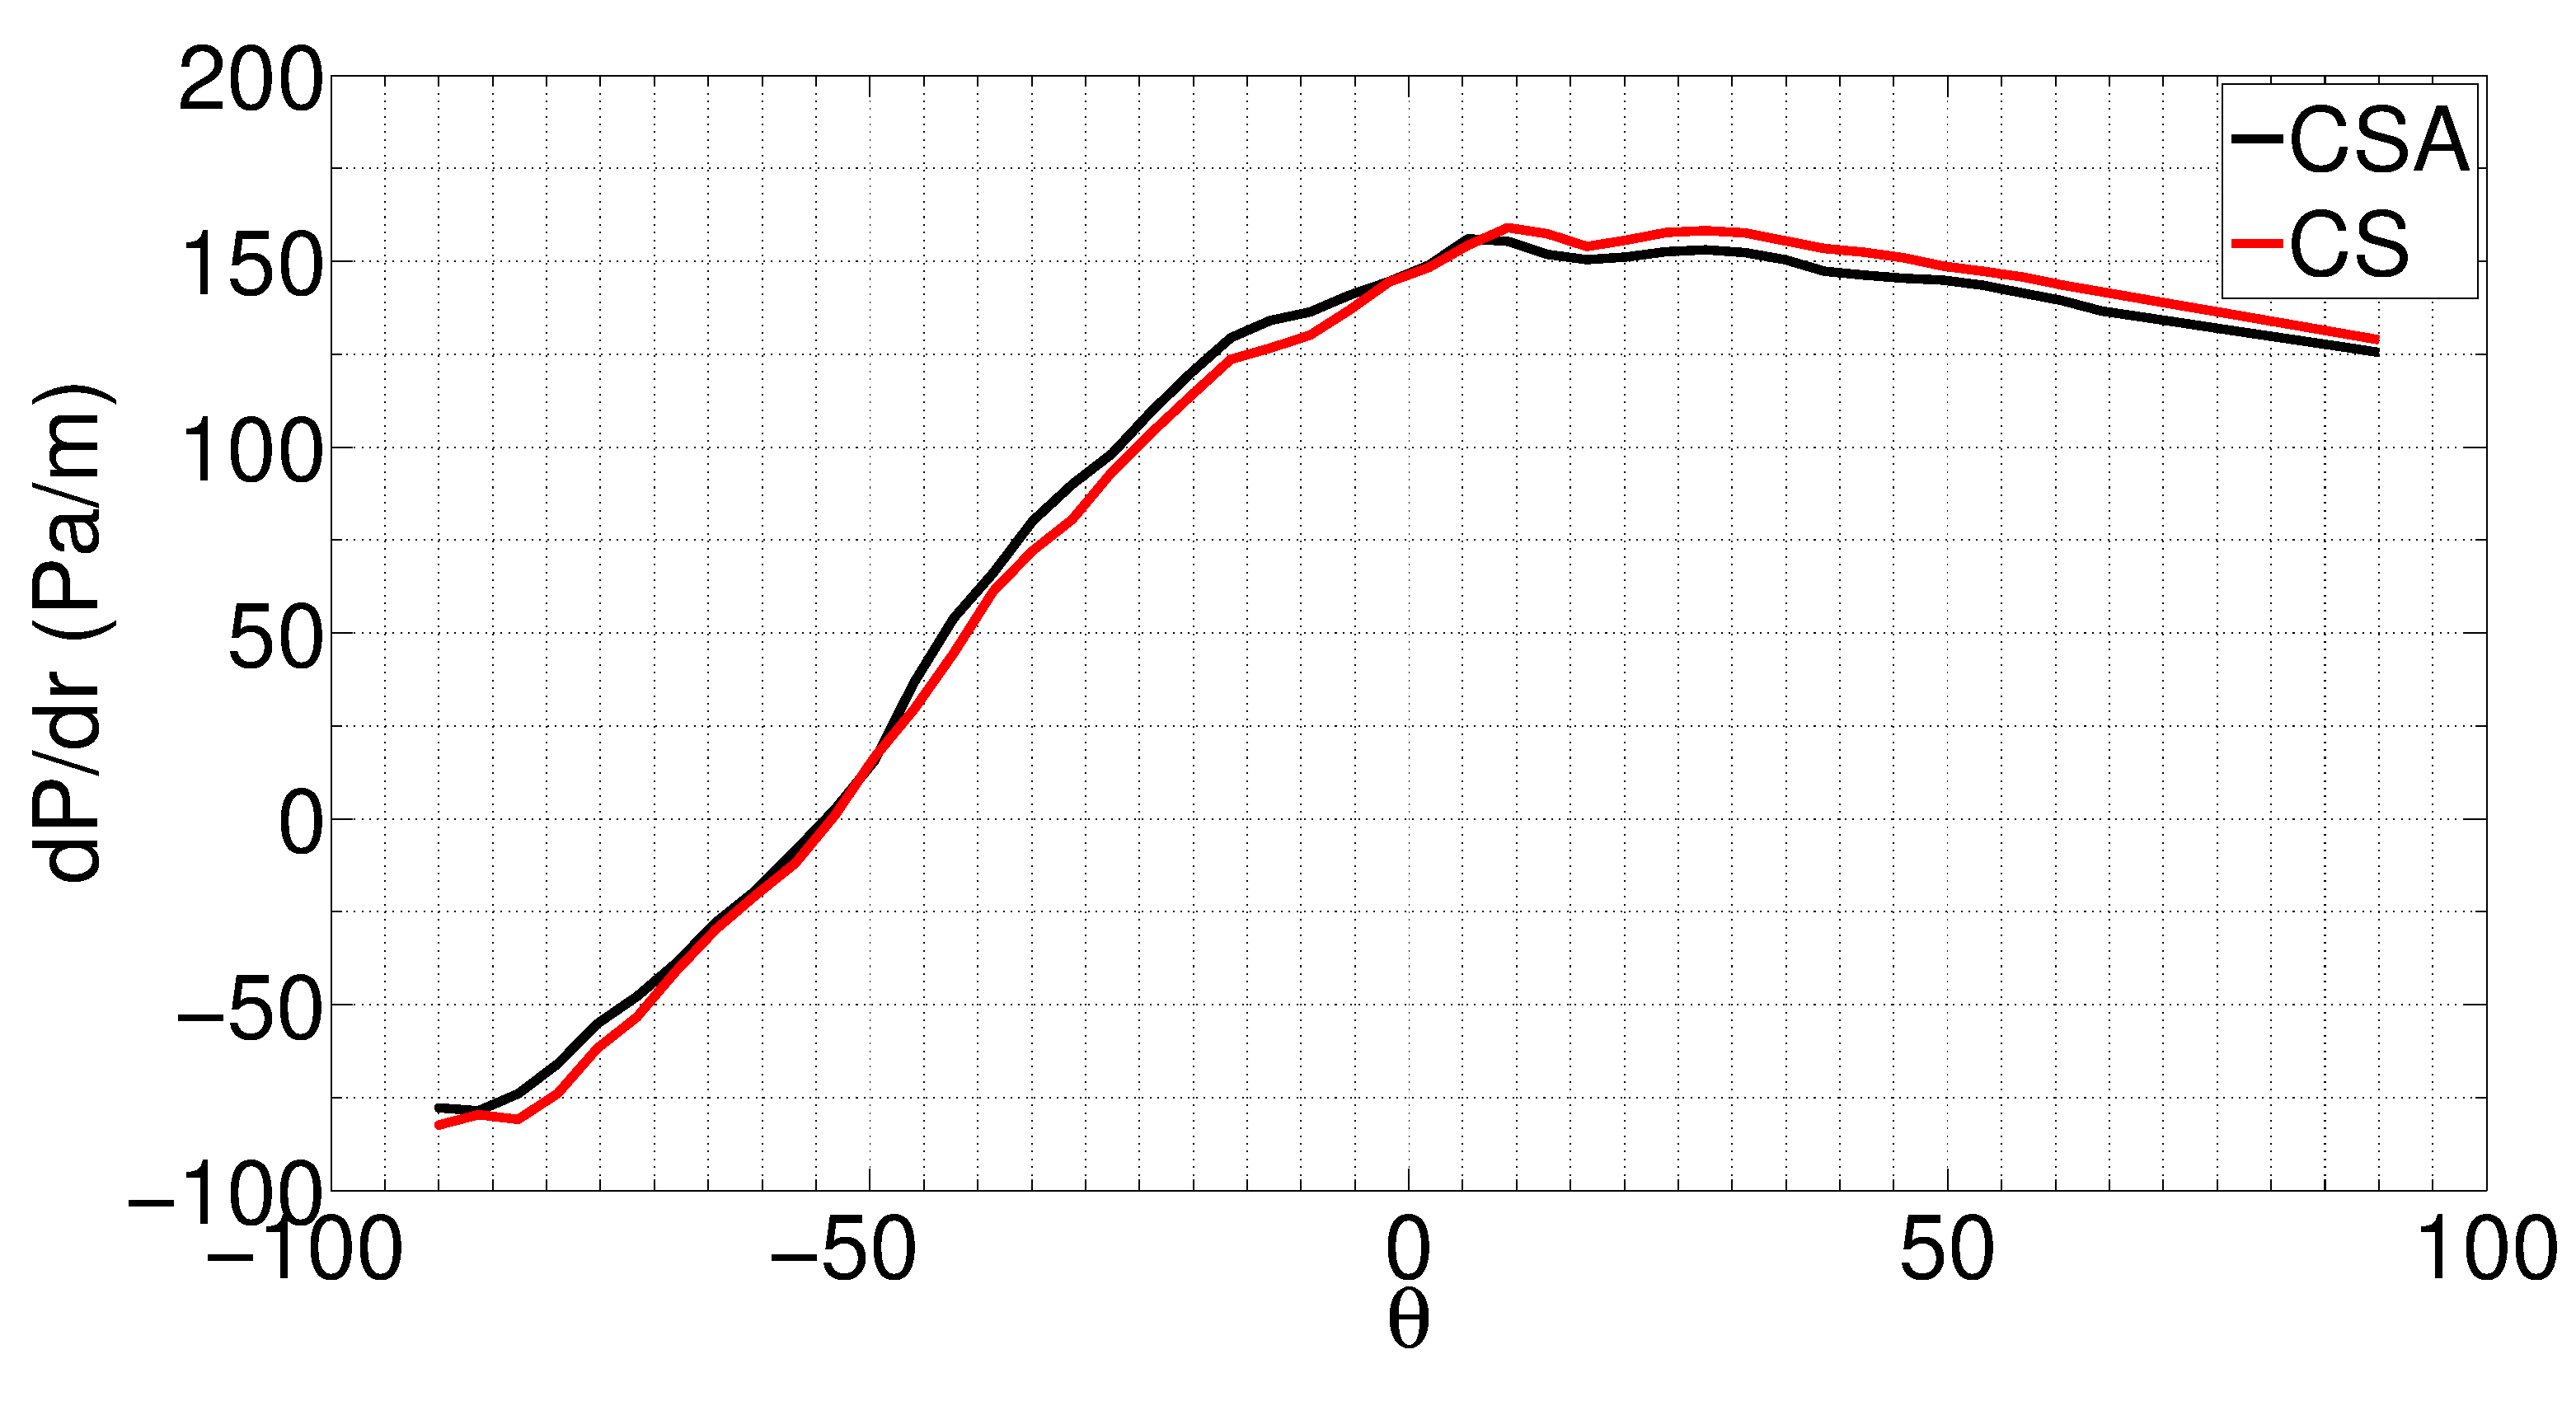
\includegraphics[width=12.00cm]{Chapter_4/figure/flow_over_cylinder/pressureSensitivityOnBoundary_RE100.eps}
    \caption{Comparison between pressure sensitivity results on the boundary for Re = 100.}
    \label{fig:C4_flowOverCylidner_pressureSensitivityOnSurface}
\end{figure}
%
